% \section{Experimental Results}
% \label{sec:experiments}

% In this section, we provide the experimental result of our algorithm, noted as {\sf CSM}. Additionally, we provide the instance-based method, noted as {\sf iCSM}, for comparison. {\sf iCSM} need to store all the instances, or we call embeddings, and thus results in a higher storage cost. However, an instance-based storage could benefit in correlation calculation and also leads to a very fast calculation of every instance towards subgraphs with backward edges because we could directly use the correlation of the ones extended to them.


% Unfortunately, the number of the instances could be exponential in worst cases, which means this number could still be very large in a not sparse data graph $G$. Except the MNI support calculation, we should also assign every instance to a group which it belongs to, which is extremely expensive. However, {\sf CSM} stores the subgraphs using the strategy of replica and avoid this huge drawback. As we demonstrate in the experimental result, {\sf CSM} has a much better performance than {\sf iCSM} in large and dense graphs. 


% Besides, we also provide the results of various input parameters, {\sf Min-sup}, hop-constraint $h$, and $k$ of {\sf Top-$k$}. All our experiments execute at GHz with $512$GB RAM and the implementation is carried out by C++.


% \spara{$\bullet$ Datasets.} Our experiments are based on $4$ datasets. The characteristics of them are listed in Table \ref{tab:datasets}.


% \spara{\em (1) Chemical}. This dataset contains the undirected graph of a chemical compound in MCF7 Dataset of X.F. Yan\cite{YH02} with 207 vertices, 215 edges, 4 distinct node labels. Each node represents a chemical atom.


% \spara{\em (2) Yeast}. This dataset contains the undirected graph of proteins using the function as label, with ~4K vertices, ~79K edges and 26 distinct node labels. 


% \spara{\em (3) DBLP}. This dataset contains the undirected graph converted from {\em file Source/dblp.txt}, with ~1M vertices, ~5.4K edges and 751 distinct node labels.


% \spara{\em (4) LastFM}. This dataset contains the undirected graph. Each vertex is a user in the FM social network and each label of each vertex is the most frequent singer or music band that this user listen to. Two users interact with each other will have a edge for connection. It has ~1.1M vertices, ~5.2M edges and ~83K distinct node labels.


% \begin{table}[tb!]
% 	\vspace{-2mm}
% 	\begin{center}
% 		\vspace{-1mm}
% 		\centering
% 		\caption{Datasets and characteristics\label{tab:datasets}}
% 		\vspace{-3mm}
% 		\begin{tabular} {cccc}
% 			\hline
% 			Datasets  & Nodes & Edges & Distinct node labels \\			 
% 			\hline 
% 			{\em Chemical}   &   207    &  205      &    4  \\
% 			{\em Yeast}   &   4138    &  78821   &   26  \\ 
% 			{\em DBLP}   &   1,064,939    &  5,350,530   &   751  \\ 
% 			{\em LastFM}   &   1,092,145   &  5,237,032   &    82,526 \\
% 			\hline
% 		\end{tabular}
% 	\end{center}
% 	\vspace{-8mm}
% \end{table}


% \spara{$\bullet$ Parameters.} There are $3$ different inputs in the problem of correlated subgraph mining. The minimum image based support {\sf Min-sup}, the $k$ value of our {\sf Top-$k$} interested results, and the hop-constraint value $h$. Increasing the value of {\sf Min-sup} results in an decrease of frequent subgraphs, increasing the value of $k$ results in an increase of output number, increasing the value of $h$ results in more subgraph pairs which we are interested in.
% \par In brief, if we ignore the value of $k$, by increasing the value of {\sf Min-sup}, we will get less correlated subgraphs. By increasing the value of $h$, we will get more correalted subgraphs.
% \par We evaluate the efficiency of the approach by setting various input parameters and analyze the time cost. The time cost is recorded from the initialization to the end of the search, the time cost of building the graph in the memory dose not count.


% \spara{$\bullet$ Memory Requirements.} The dataset {\em DBLP} with input parameters, {\sf Min-sup}= $5000$, $k=200$, $h=2$ has the largest memory cost among all our experiments except setting $h=3$ of our {\sf CSM} approach, which is $512$GB$\times 1.8\%=9.216$GB.
% \par Compared with this acceptable memory cost, the algorithm {\sf iCSM} has a memory cost of $512$GB$\times 8.2\%=41.984$GB, after $8$ hours running and mined only hundreds of frequent subgraphs during processing the dataset {\em DBLP}. Even if we are patient enough to wait for the result of {\sf iCSM}, it is definitely about to crash before it reach the ceasing condition. This fact demonstrates that the memory cost of instance based method could only be tolerated when the data graph is sparse. However, our replica based storage has a acceptable memory cost towards the data graph which is both large and dense. 


% \begin{figure}[t!]
% \vspace{-2mm}
% \centering
% \subfigure[{\scriptsize {\sf Top-$3$} correlation of {\em Chemical}}]{
% 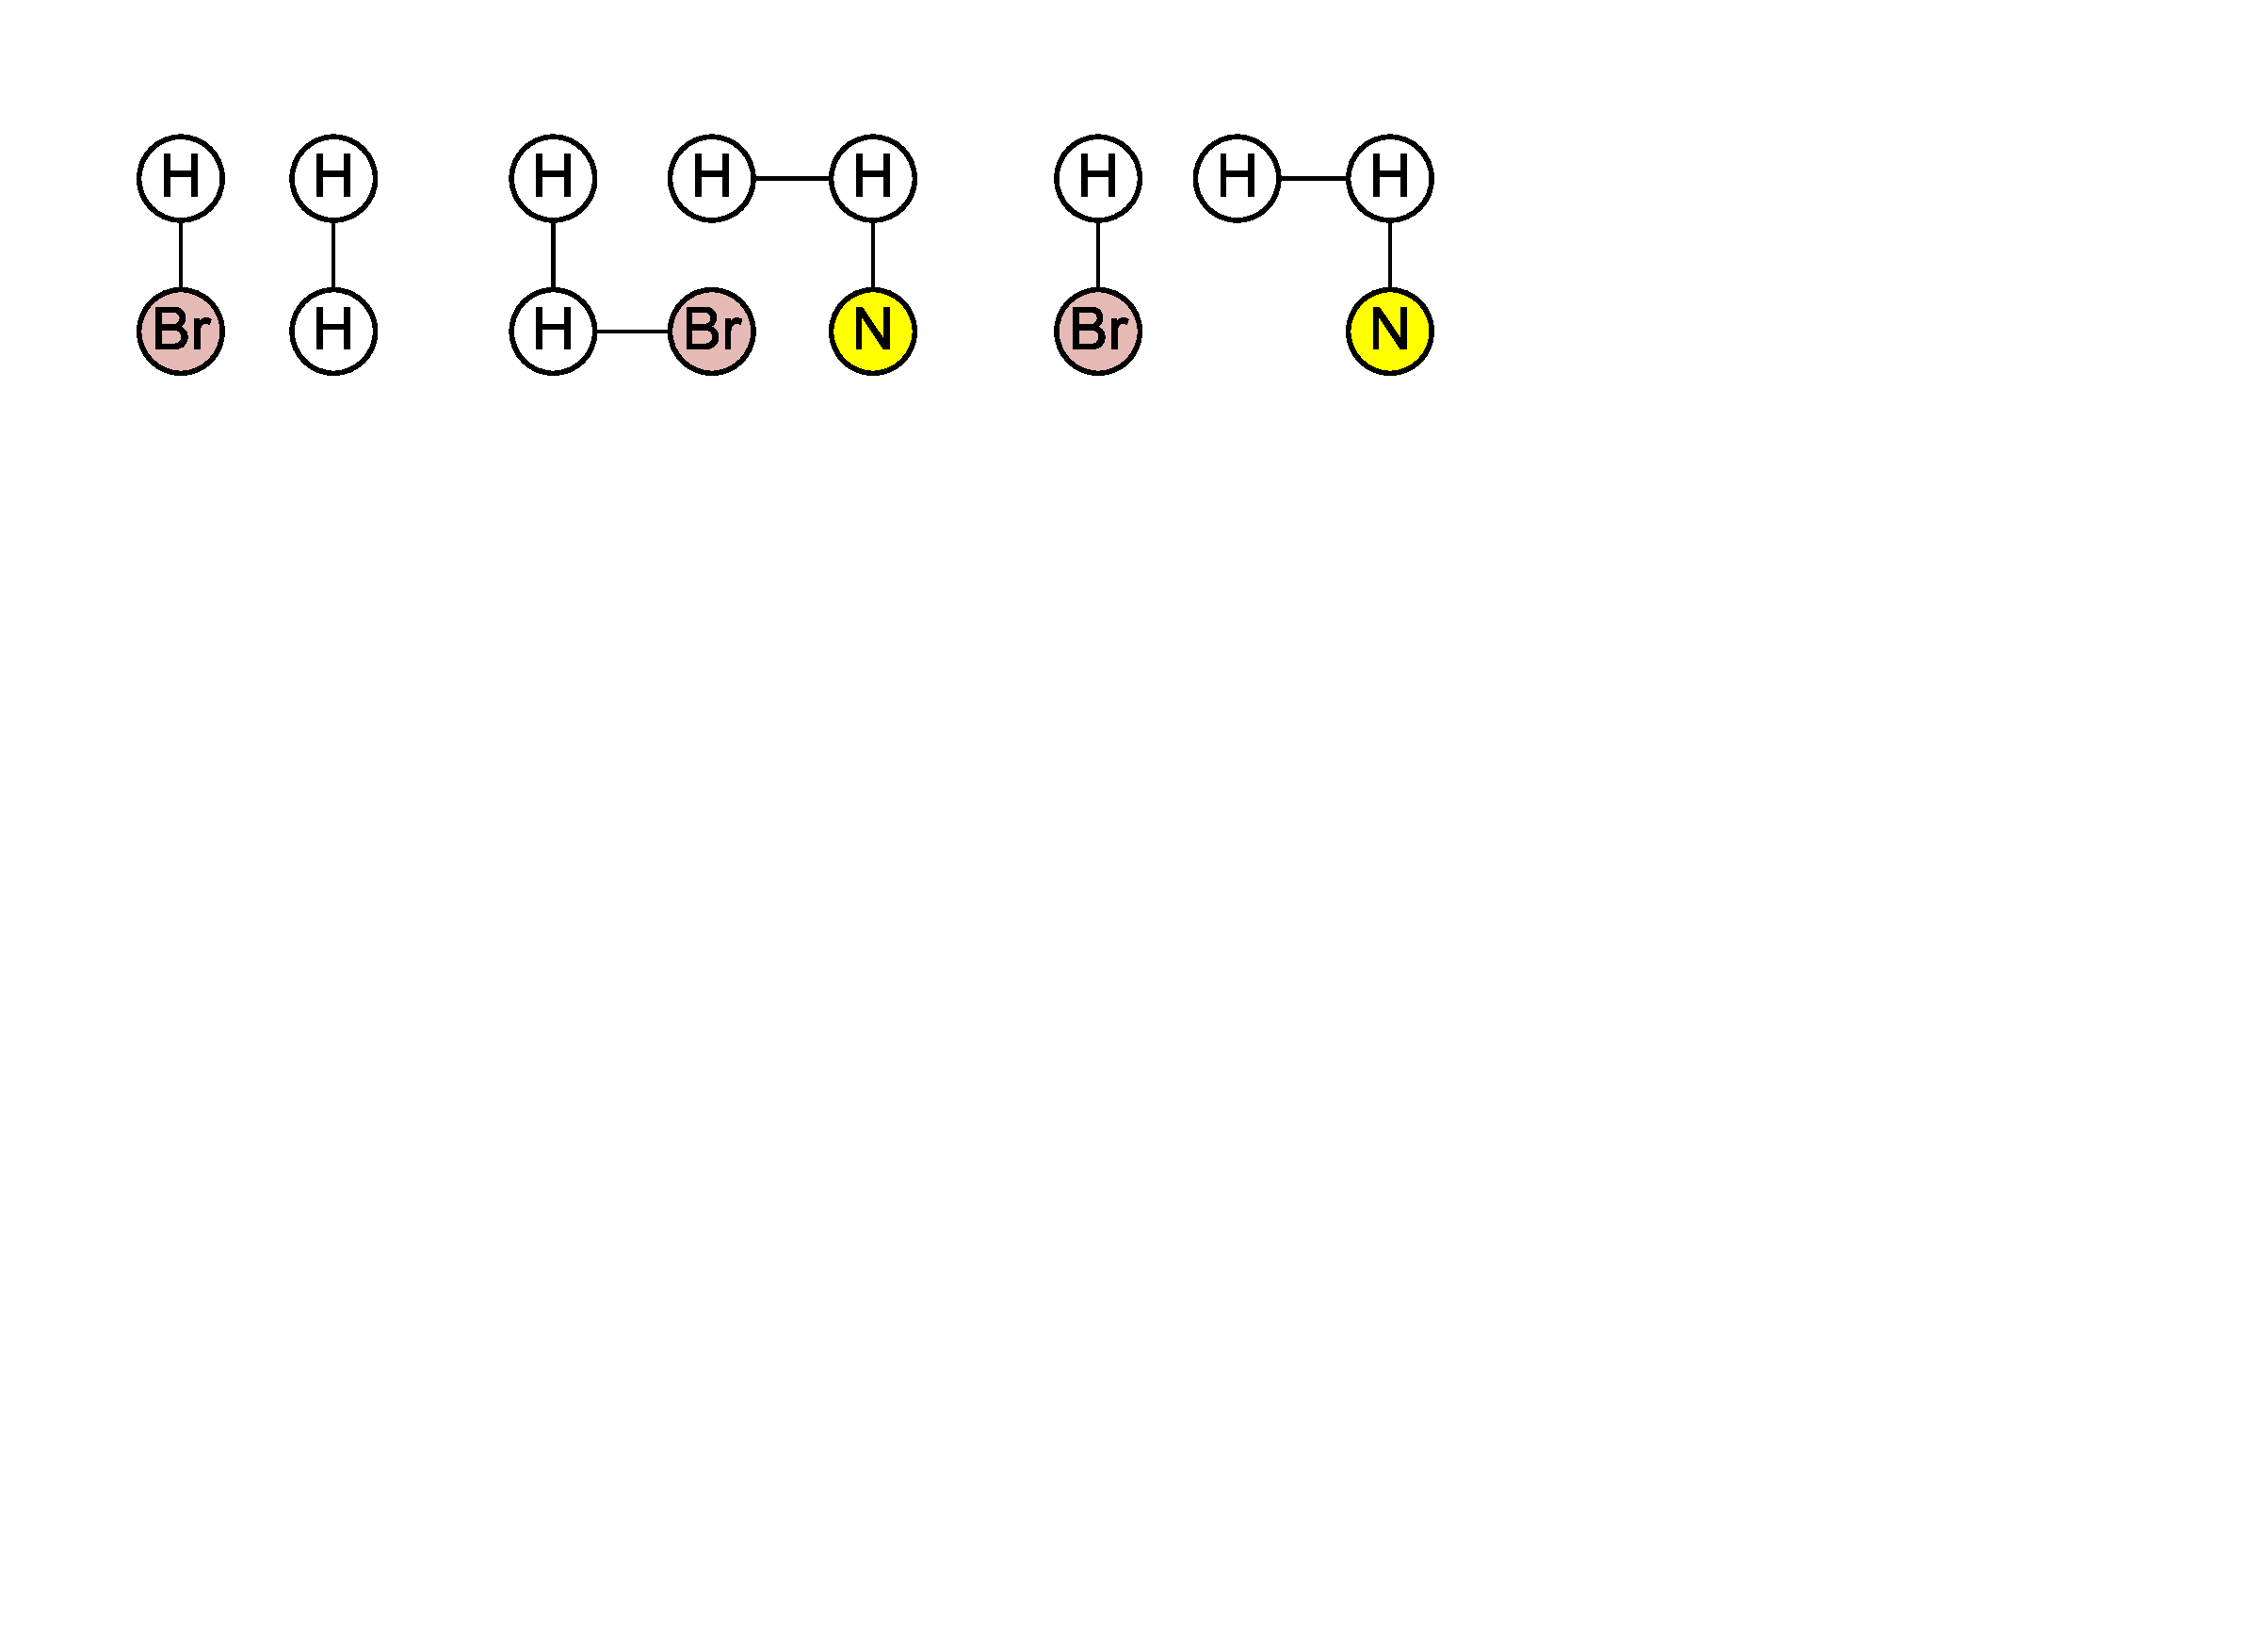
\includegraphics[scale=0.35]{images/tp_chemical}
% \label{fig:tp_chemical}
% }
% \subfigure[{\scriptsize {\sf Top-$3$} correlation of {\em Yeast}}]{
% 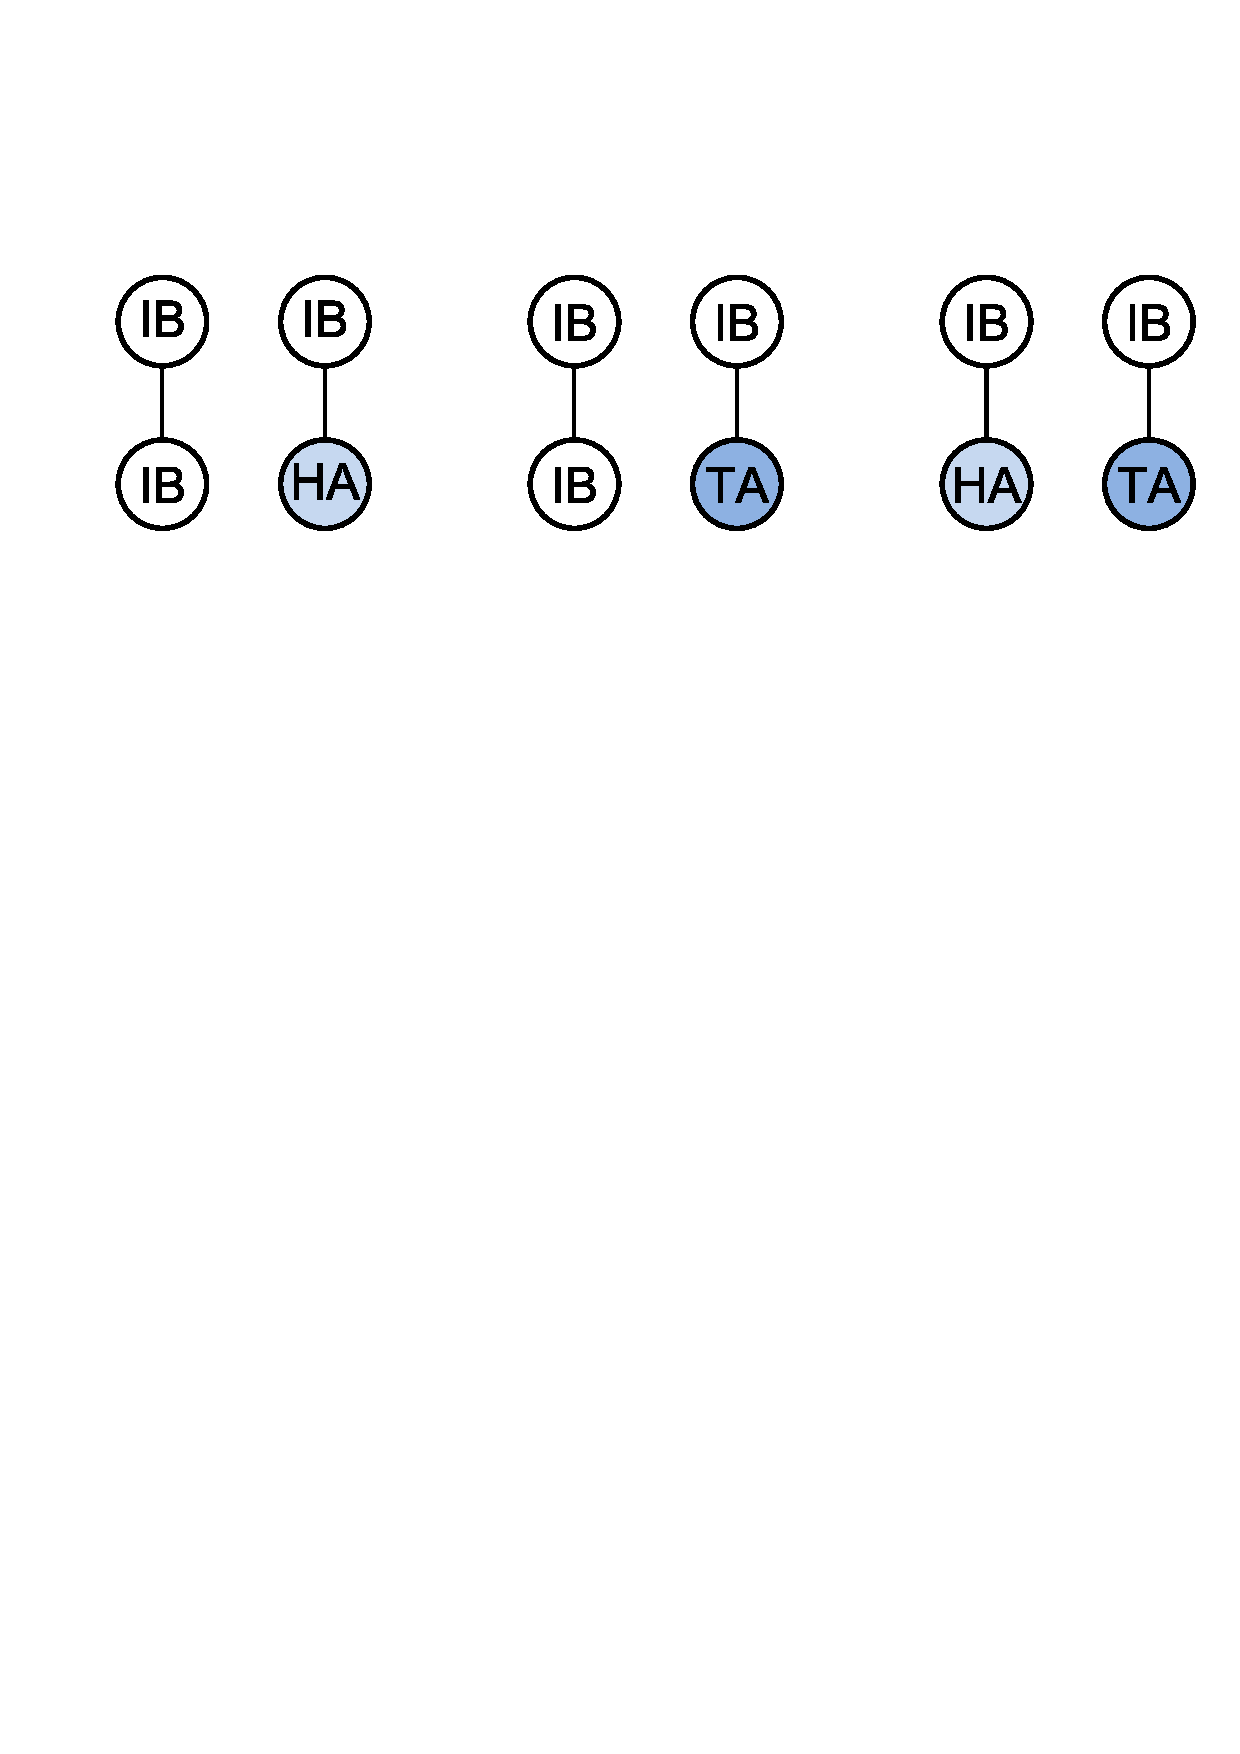
\includegraphics[scale=0.35]{images/tp_yeast}
% \label{fig:tp_yeast}
% }
% \subfigure[{\scriptsize {\sf Top-$3$} correlation of {\em DBLP}}]{
% 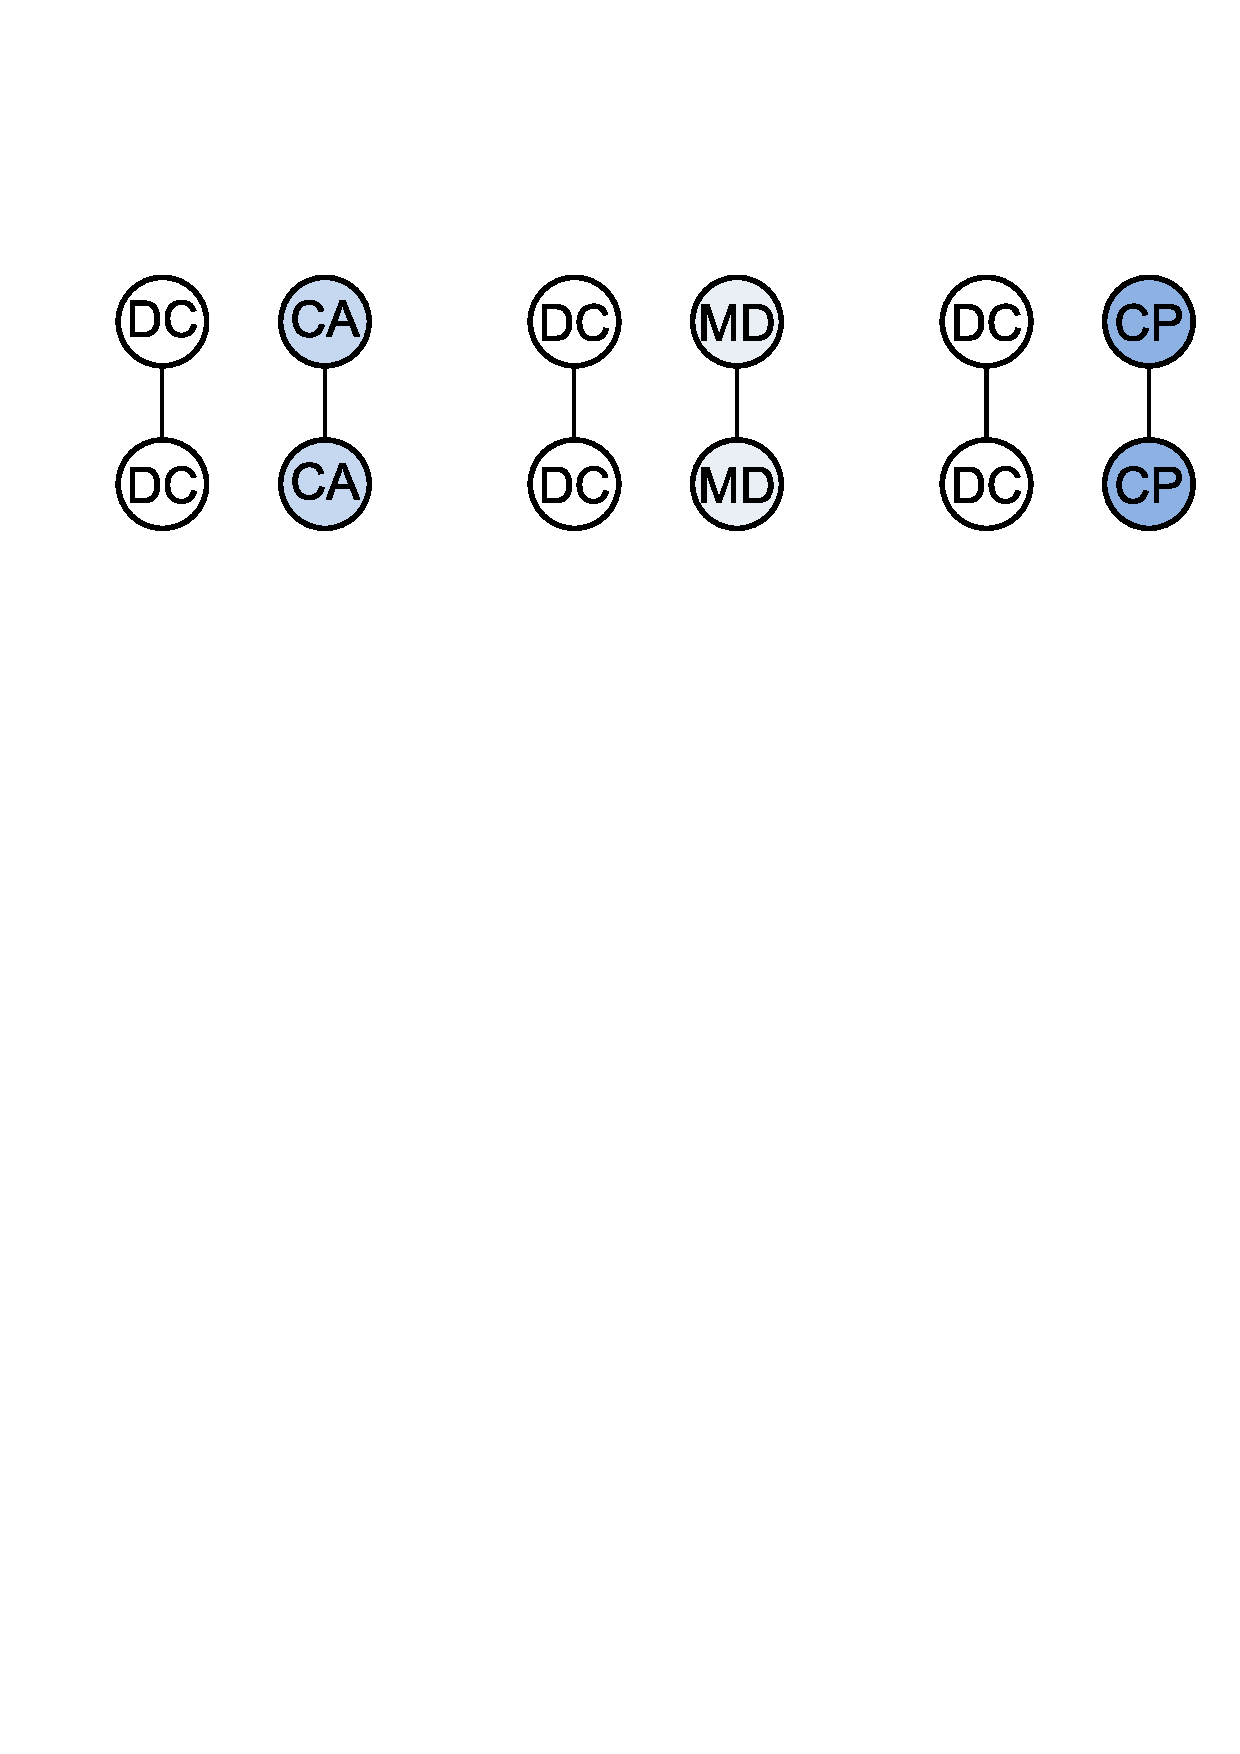
\includegraphics[scale=0.35]{images/tp_dblp}
% \label{fig:tp_dblp}
% }
% \subfigure[{\scriptsize {\sf Top-$3$} correlation of {\em LastFM}}]{
% 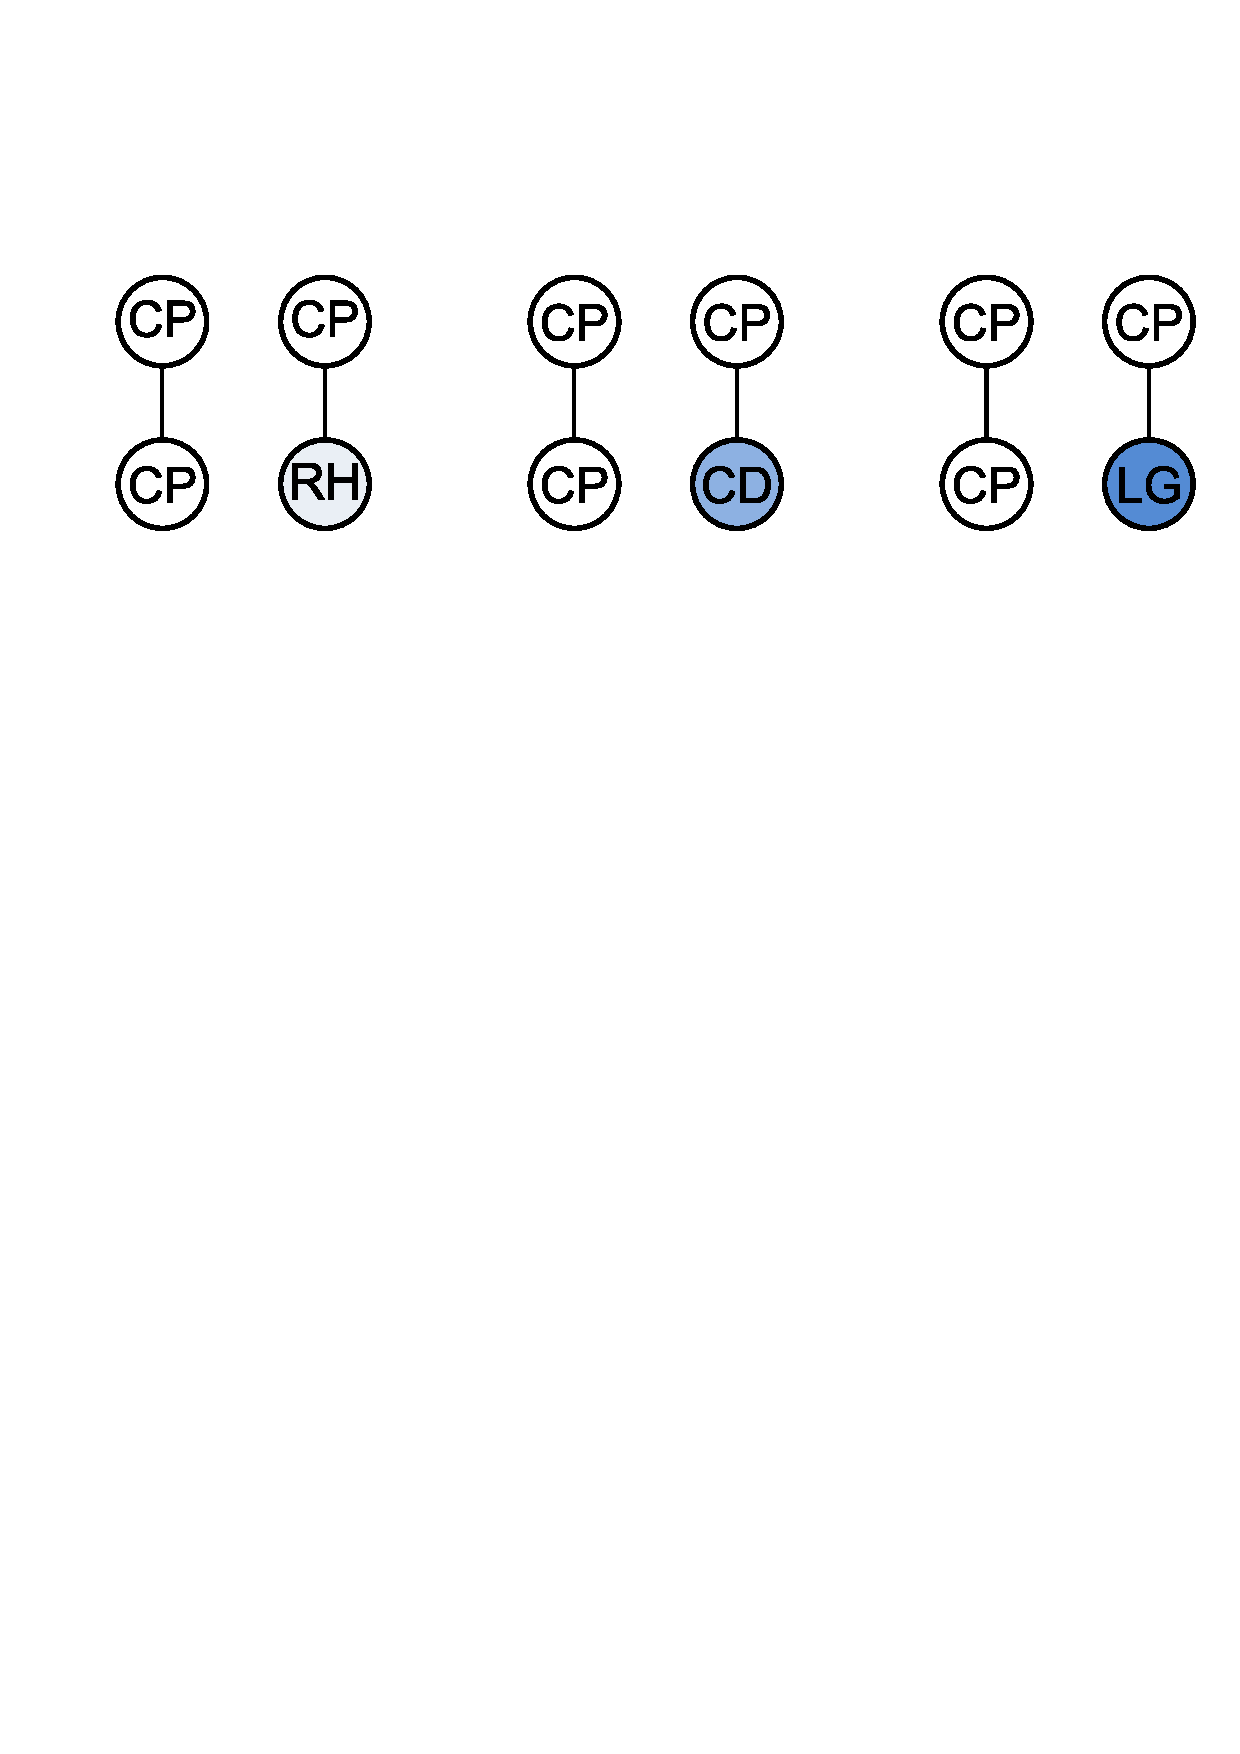
\includegraphics[scale=0.35]{images/tp_lastfm}
% \label{fig:tp_lastfm}
% }
% \subfigure[{\scriptsize {\sf Top-$3$} correlation of {\em LastFM}}]{
% 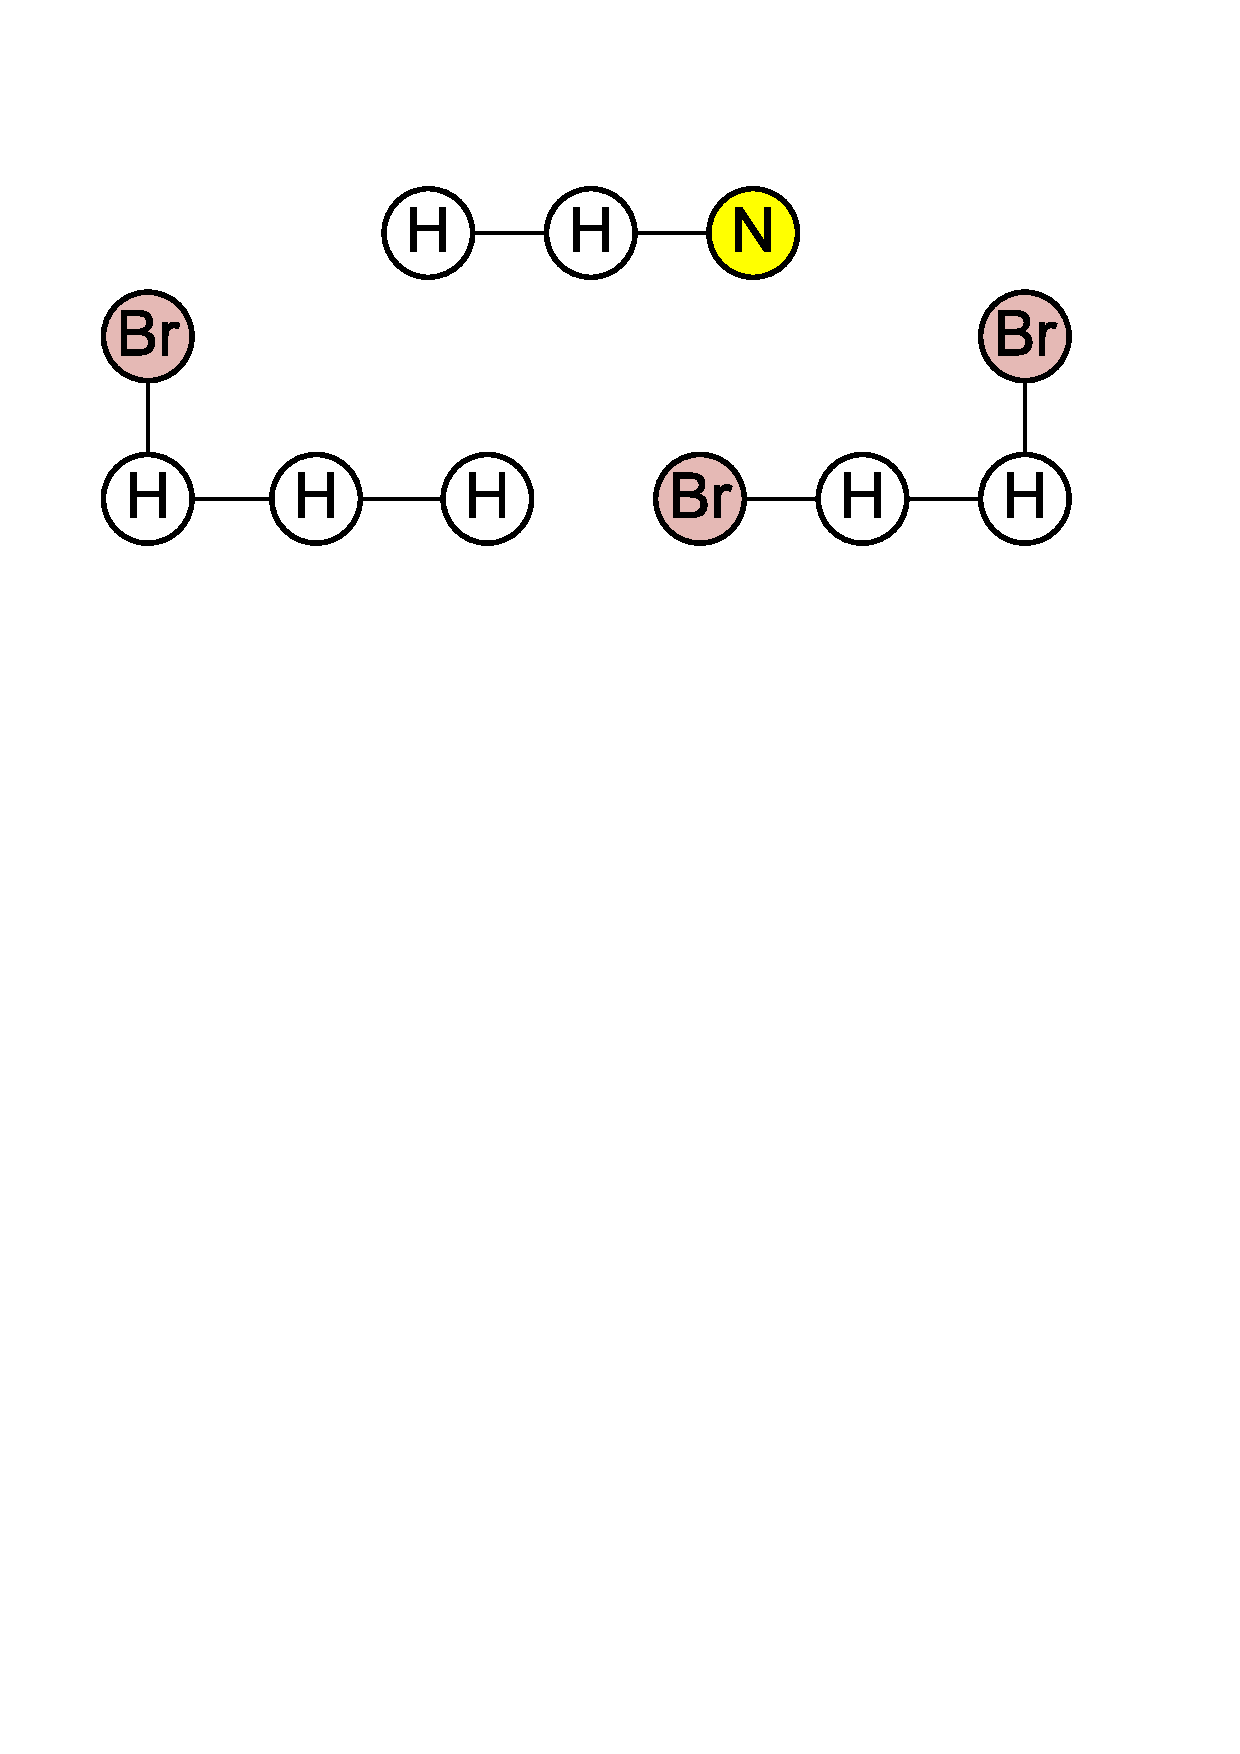
\includegraphics[scale=0.35]{images/tp_group}
% \label{fig:tp_group}
% }
% \vspace{-2mm}
% \caption{\scriptsize {\sf Top-$3$ correlations of datasets {\em (1)(2)(3)(4)}}.}
% \label{fig:tp}
% \vspace{-2mm}
% \end{figure}


% \spara{$\bullet$ Result Analysis.} For the datasets like {\em DBLP} which is very large but less dense, the number of the subgraphs dose not grow very quickly when the value of {\sf Min-sup} decrease. For the datasets like {\em Yeast} which is very dense, the number of the subgraphs increase at a multiple speed. However, the number of correlation is also much higher in dense graphs than that in sparse graphs because more degree also leads to the higher possibility of the correlations, which leads to an early termination and succeed to keep the efficiency of our approach.


% Besides, we provide the total number of correlations with different input parameters {\sf Min-sup} and $h$, as Table \ref{tab:k-result}. The result is also easy to infer, which is, with lower {\sf Min-sup} or larger $h$, the total number of correlations would increase.

% \begin{table}[tb!]
% 	\vspace{4mm}
% 	\begin{center}
% 		\vspace{-1mm}
% 		\centering
% 		\caption{Correlated Subgraphs of various {\sf Min-sup} and $h$\label{tab:k-result}}
% 		\vspace{-3mm}
% 		\begin{tabular} {cccccc}
% 			\hline
% 			{Dataset} & {\sf Min-sup}  & $h=0$ & $h=1$ & $h=2$ & $h=3$ \\			 
% 			\hline 
% 			\multirow{3}{*}{Chemical} & 20 & 5 & 5 &  5 & 5 \\
% 			& 25   & 1 & 2 & 2 & 2 \\ 
% 			& 30   & 1 & 1 & 1 & 1 \\ 
% 			\hline 
% 			\multirow{3}{*}{Yeast} & 300 & 19 & 45 & 50 & 50 \\
% 			& 330   & 8 & 21 & 21 & 21 \\
% 			& 360   & 2 & 7 & 10 & 10 \\ 
% 			\hline 
% 			\multirow{3}{*}{DBLP} & 7000   &  2 & 31 & 146 & 311\\ 
% 			& 8000   &  0 & 16 & 94 & 196 \\
% 			& 9000   &  0 & 7 & 10 & 10 \\
% 			\hline 
% 			\multirow{3}{*}{LastFM} & 600   & 18 & 26 & 488 & 765 \\
% 			& 700   &  11 & 13 & 223 & 311 \\ 
% 			& 800   &  6 & 7 & 116 & 174 \\ 
% 			\hline
% 		\end{tabular}
% 	\end{center}
% 	\vspace{-8mm}
% \end{table}


% \begin{table}[tb!]
% 	\vspace{4mm}
% 	\begin{center}
% 		\vspace{-1mm}
% 		\centering
% 		\caption{Time cost comparison of {\sf CSM} and {\sf iCSM}\label{tab:icsm}}
% 		\vspace{-3mm}
% 		\begin{tabular} {ccccc}
% 			\hline
% 			Datasets & {\em Chemical} & {\em Yeast} & {\em DBLP} & {\em LastFM} \\			 
% 			\hline 
% 			{\sf CSM}   &  0.1 & 14 & 507 & 823 \\
% 			{\sf iCSM}   &  0.2 & over 10000 & over 10000 & over 10000 \\ 			
% 			\hline
% 		\end{tabular}
% 	\end{center}
% 	\vspace{-4mm}
% \end{table}


% \spara{$\bullet$ Comparison with {\sf iCSM}.} In Table \ref{tab:icsm}, we present the time cost (in sec) of all the datesets with setting {\sf Min-sup} $=20$ of {\em (1)}, {\sf Min-sup} $=200$ of {\em (2)}, {\sf Min-sup} $=5000$ of {\em (3)}, {\sf Min-sup} $=200$ of {\em (4)}, and all the datasets with $h=2$, $k=5$. The approach {\sf iCSM} could have a decent performance when the dataset is not dense, or relatively small, as the experiment on dataset {\em Chemical}. However, when the dataset becomes dense, it has to tackle with the exponential growth of the number of the instances, which is very expensive. In {\em Yeast} dataset, the most frequent single edge subgraph $Q$ has a MNI support $\sigma(Q)=1.4$K, but with the number of the instances $11$K. This number continues to grow at this speed and results in nearly $0.1$ million of the most frequent two edge subgraph. Suppose this number of the instances is $n$, after MNI support is calculated in $O(n)$ time, we have to spend another $O(n^2)$ time to finish the grouping process, which assigns each instance to a particular group. Eventually, this rapid growth of instance number leads to an unacceptable time cost of the approach {\sf iCSM}.


% \spara{$\bullet$ Result on large datasets.} We provide the experimental result on two large datasets. From our empirical result, if there are enough $k$ correlations eligible, the time cost of all the datasets setting $h=0$ and $h=1$ could have no difference larger than $1$ sec. This is because through $h=1$ has a time increase from $h=0$, the total time cost at correlation calculation still does not dominate the total time cost. However, setting $h=2$ would receive a much higher time cost because the time cost of correlation calculation begins to dominate the total cost. However, when $h=3$, the time cost becomes extremely expensive and also has the memory cost over $256$GB. As a result, an approximation mining approach need to be proposed.


% \begin{figure}[t!]
% \vspace{-2mm}
% \centering
% \subfigure[{\scriptsize {\sf Min-sup} = $10$ in {\em Chemical}}]{
% 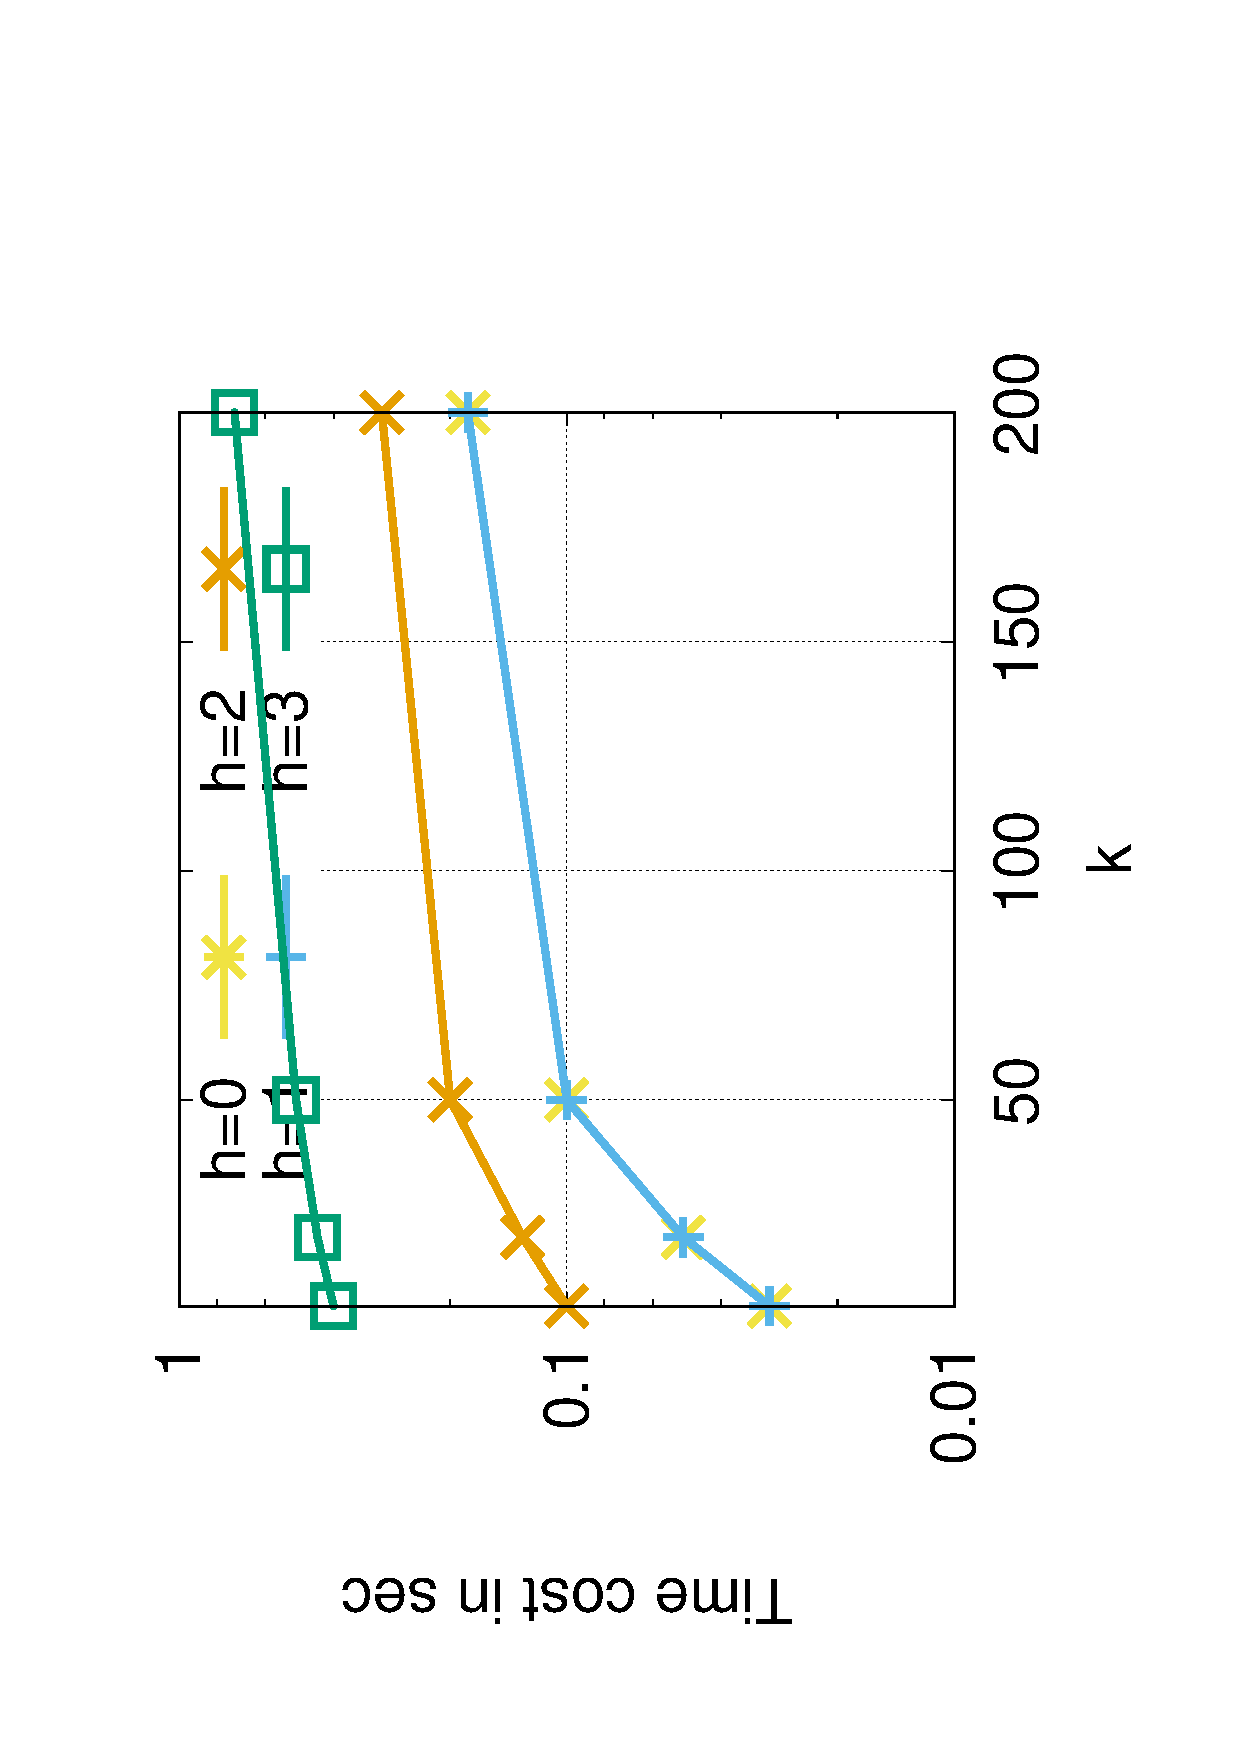
\includegraphics[scale=0.17, angle=270]{img2/exp_chemical}
% \label{fig:exp_chemical}
% }
% \subfigure[{\scriptsize {\sf Min-sup} = $200$ in {\em Yeast}}]{
% 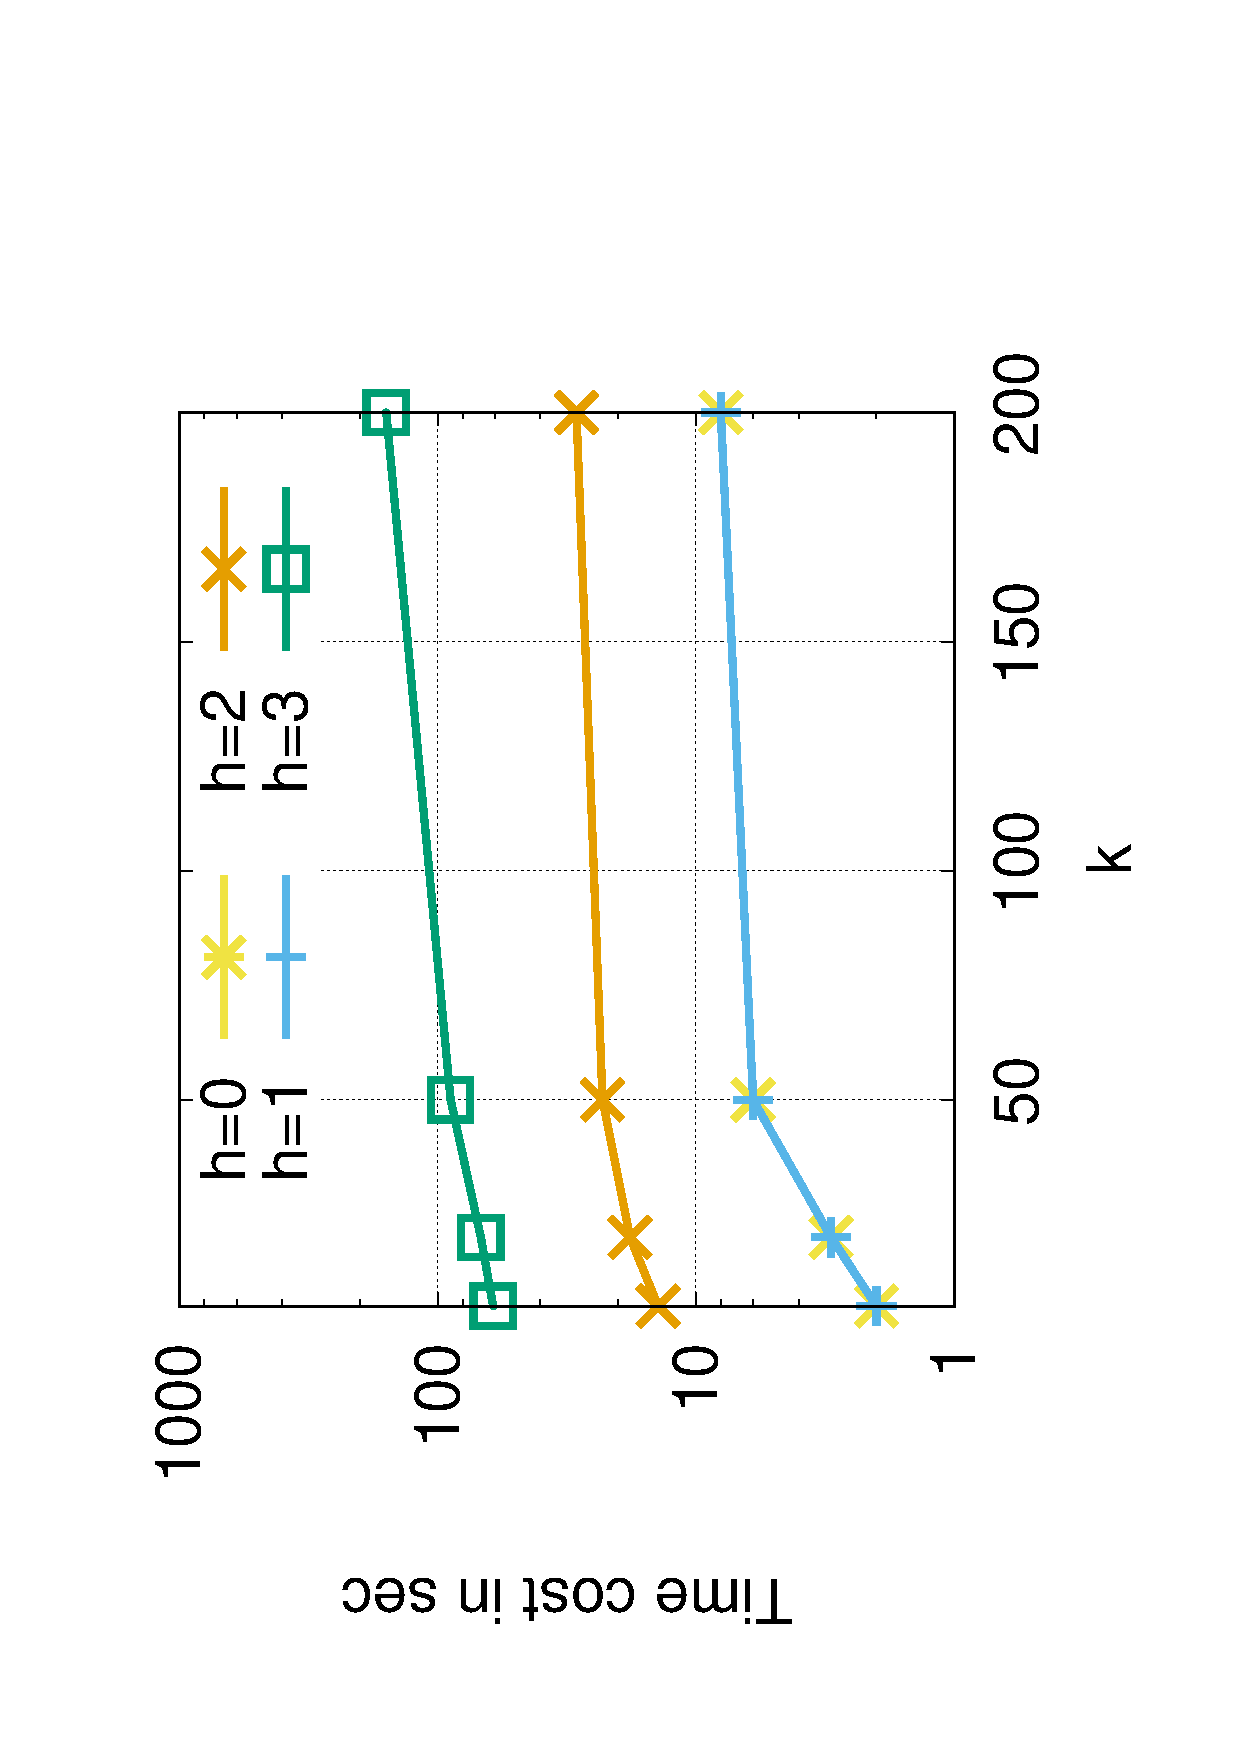
\includegraphics[scale=0.17, angle=270]{img2/exp_yeast}
% \label{fig:exp_yeast}
% }
% \subfigure[{\scriptsize {\sf Min-sup} = $5000$ in {\em DBLP}}]{
% 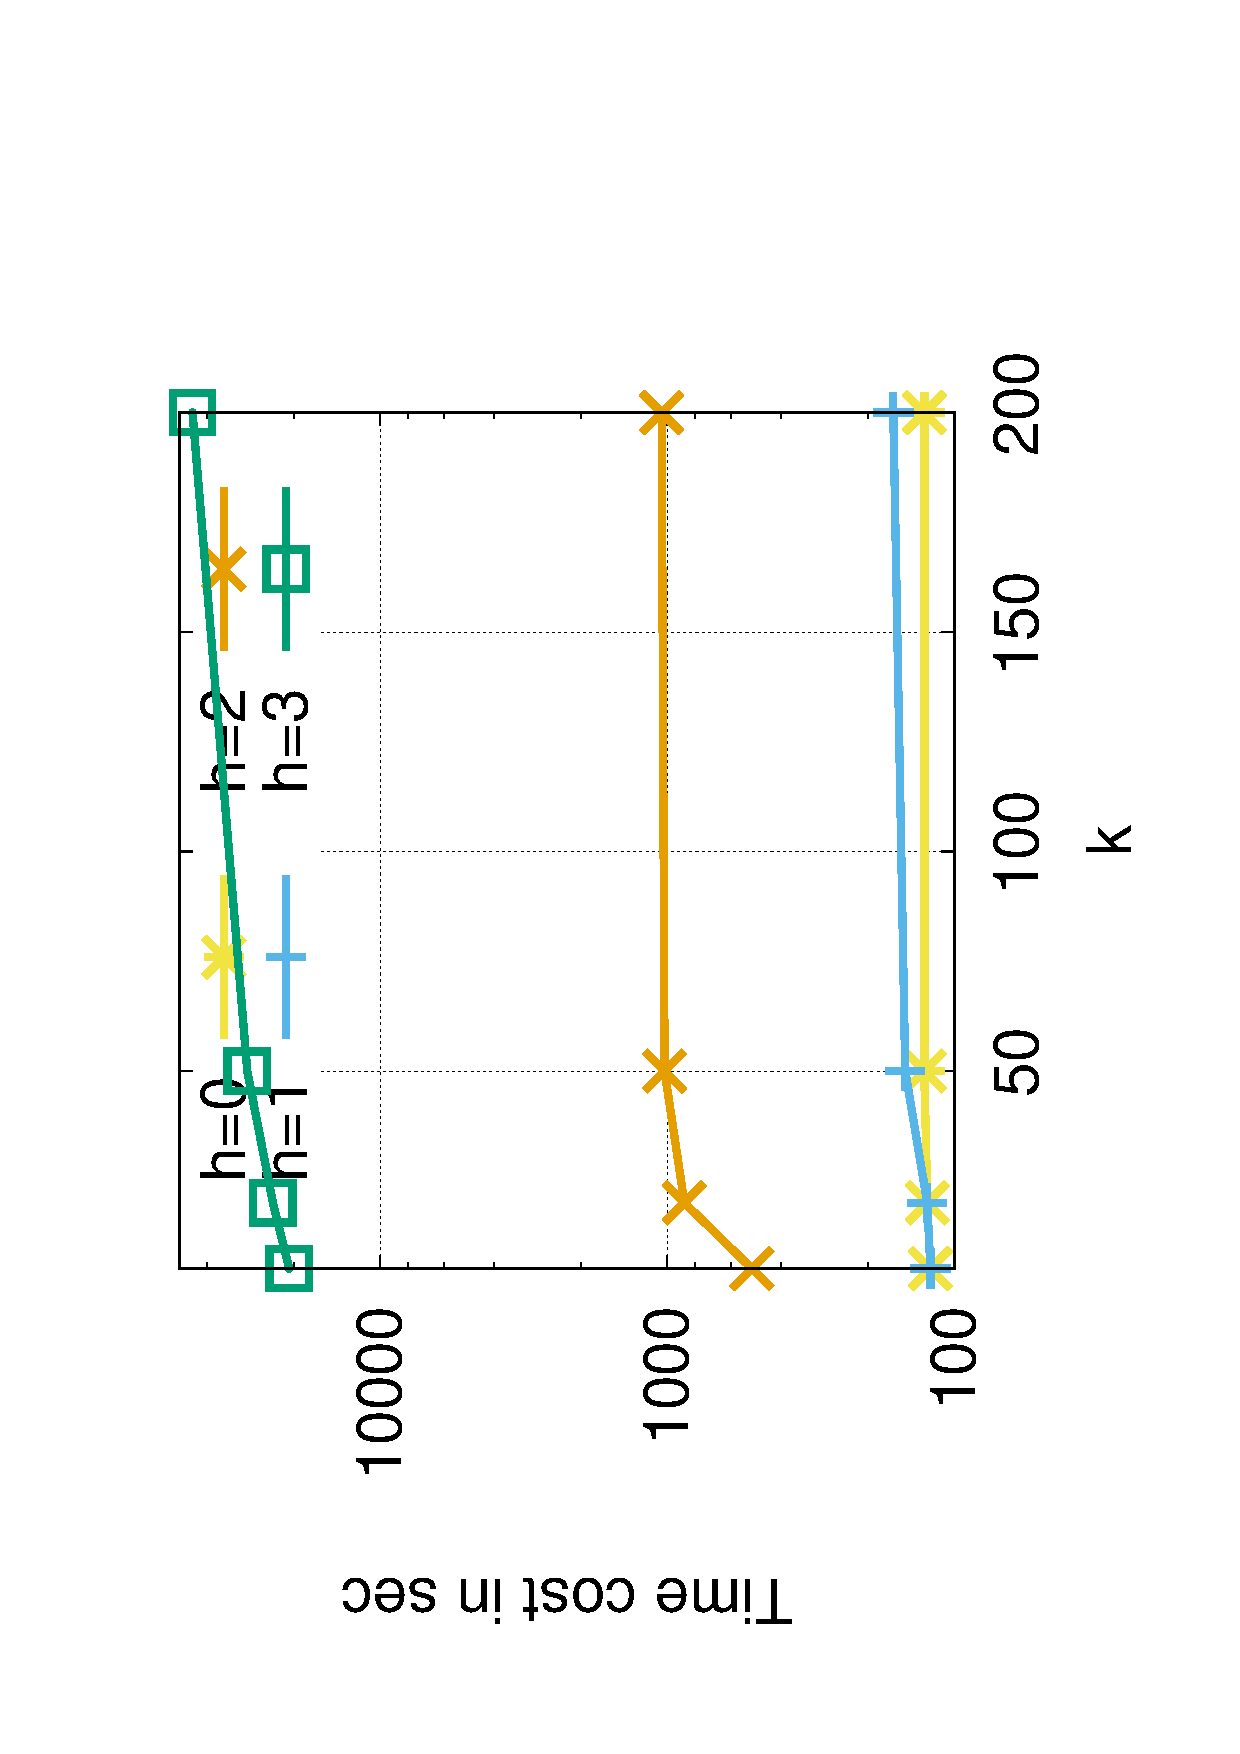
\includegraphics[scale=0.17, angle=270]{img2/exp_dblp}
% \label{fig:exp_dblp}
% }
% \subfigure[{\scriptsize {\sf Min-sup} = $200$ in {\em LastFM}}]{
% 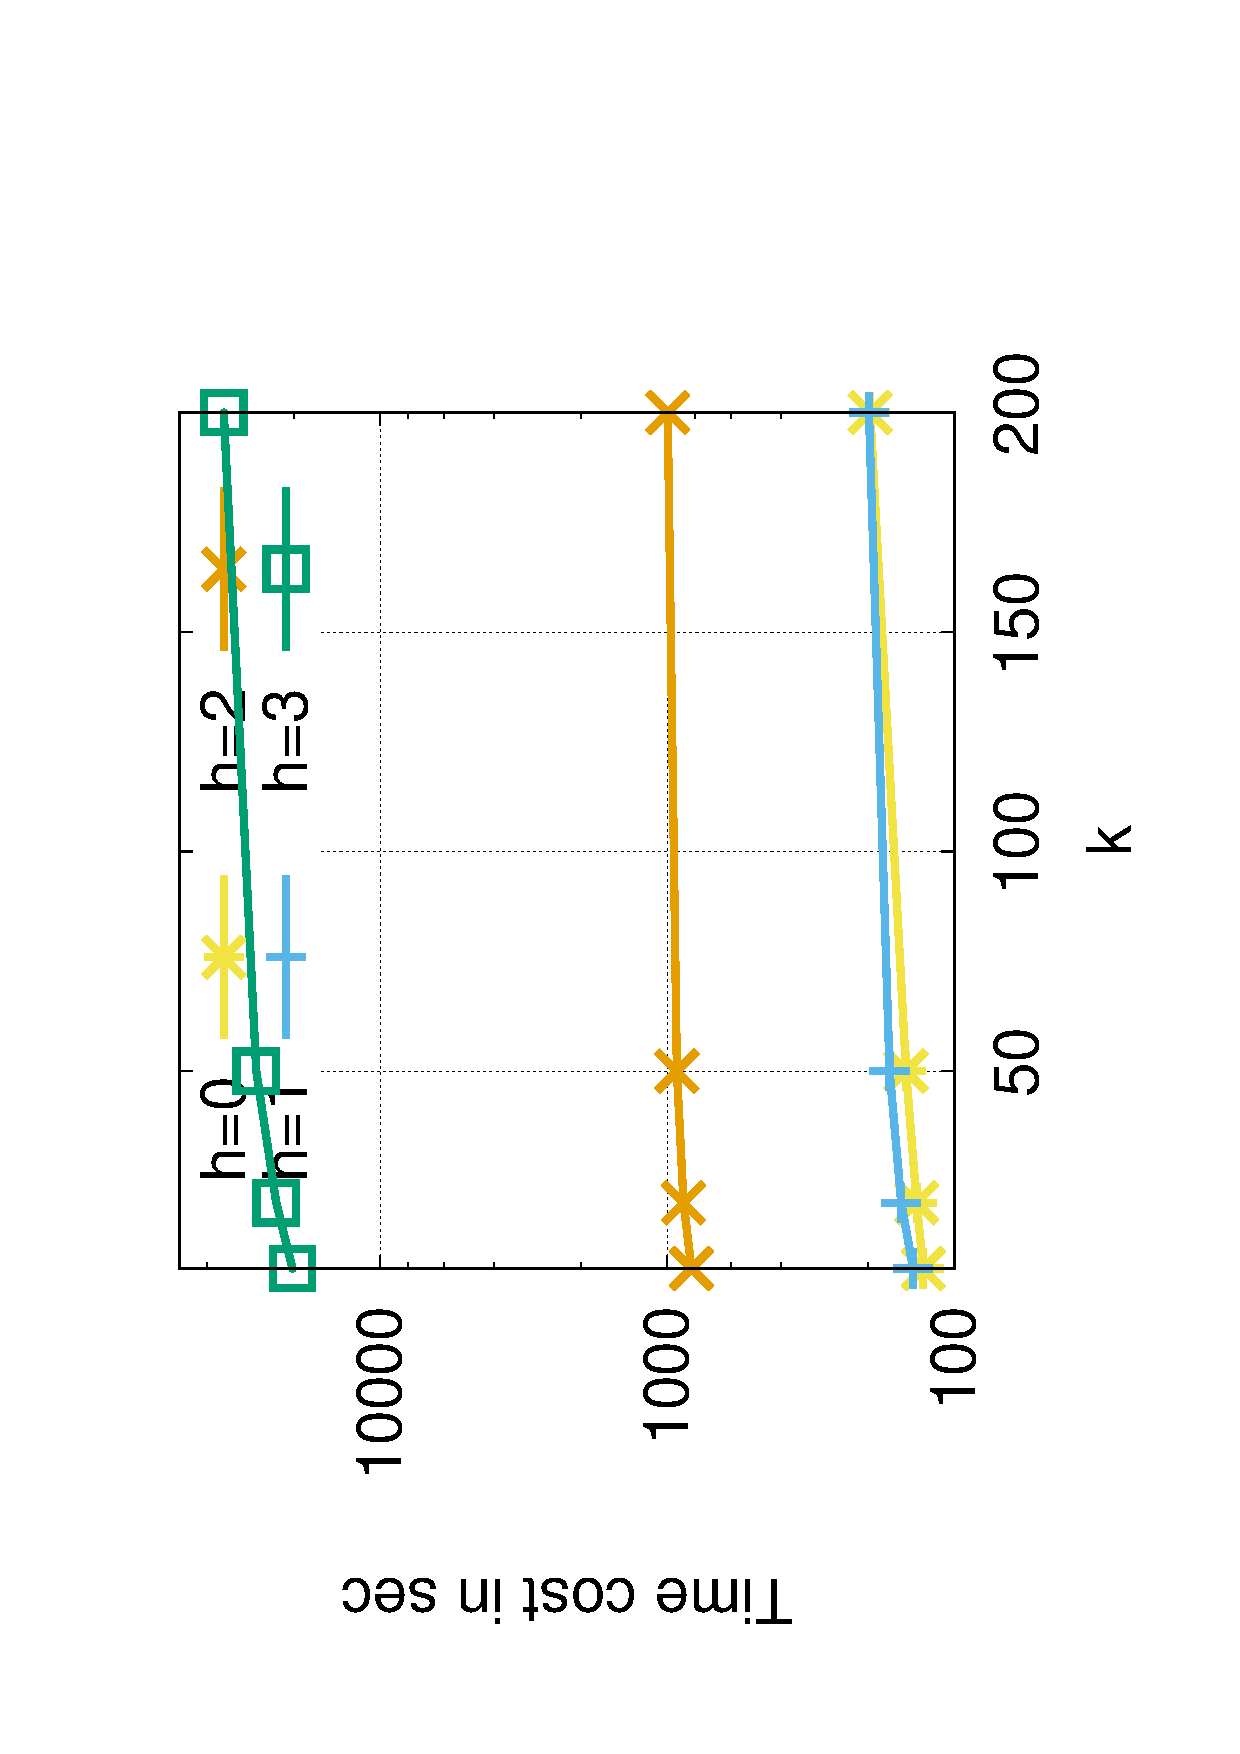
\includegraphics[scale=0.17, angle=270]{img2/exp_lastfm}
% \label{fig:exp_lastfm}
% }
% \vspace{-2mm}
% \caption{\scriptsize Experimental results on datasets {\em (1)(2)(3)(4)}.}
% \label{fig:exp}
% \vspace{-6mm}
% \end{figure}


% \begin{figure}[t!]
% \vspace{4mm}
% \centering
% \subfigure[{\scriptsize A subgraph pattern}] {
% 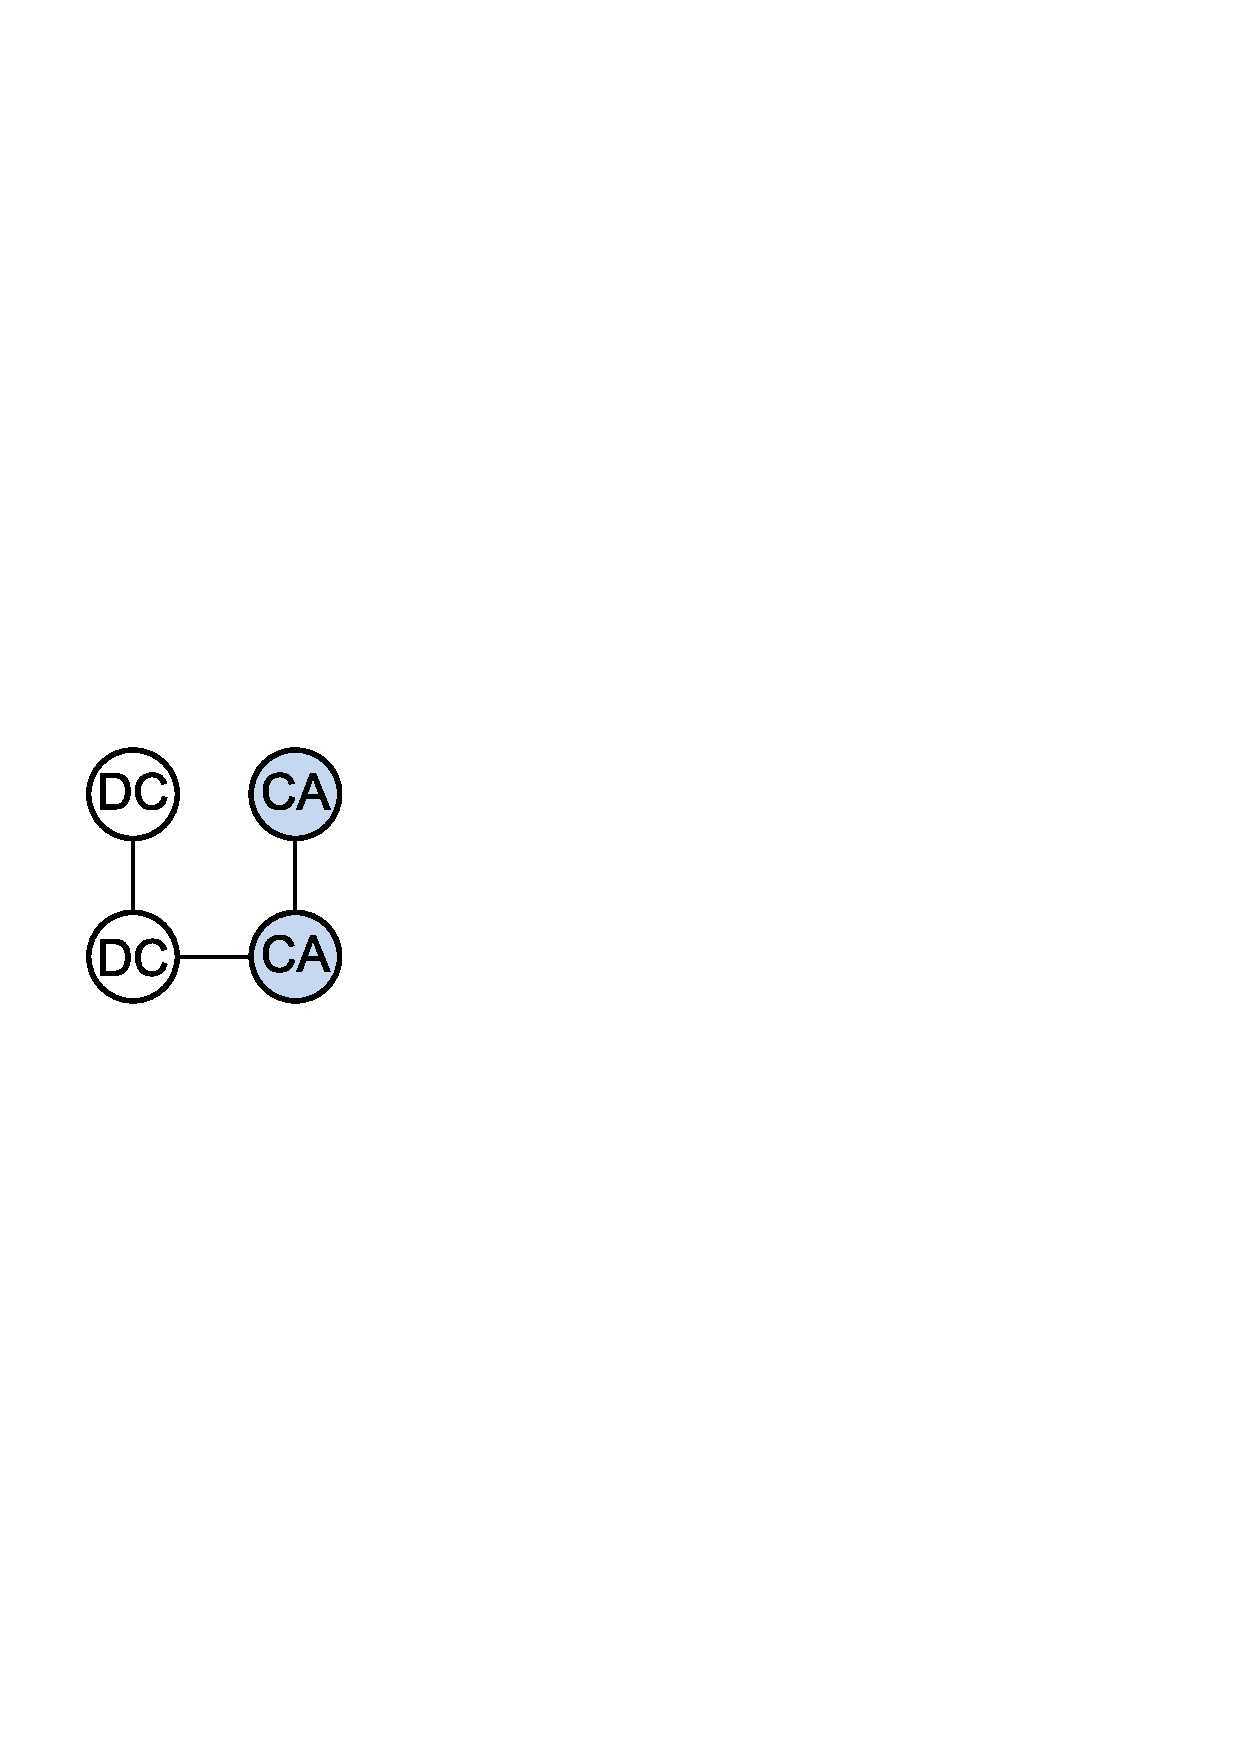
\includegraphics[scale=0.35]{images/result1}
% \label{fig:result1}
% }
% \subfigure[{\scriptsize A correlation with larger subgraph size in {\em Chemical}}]  {
% 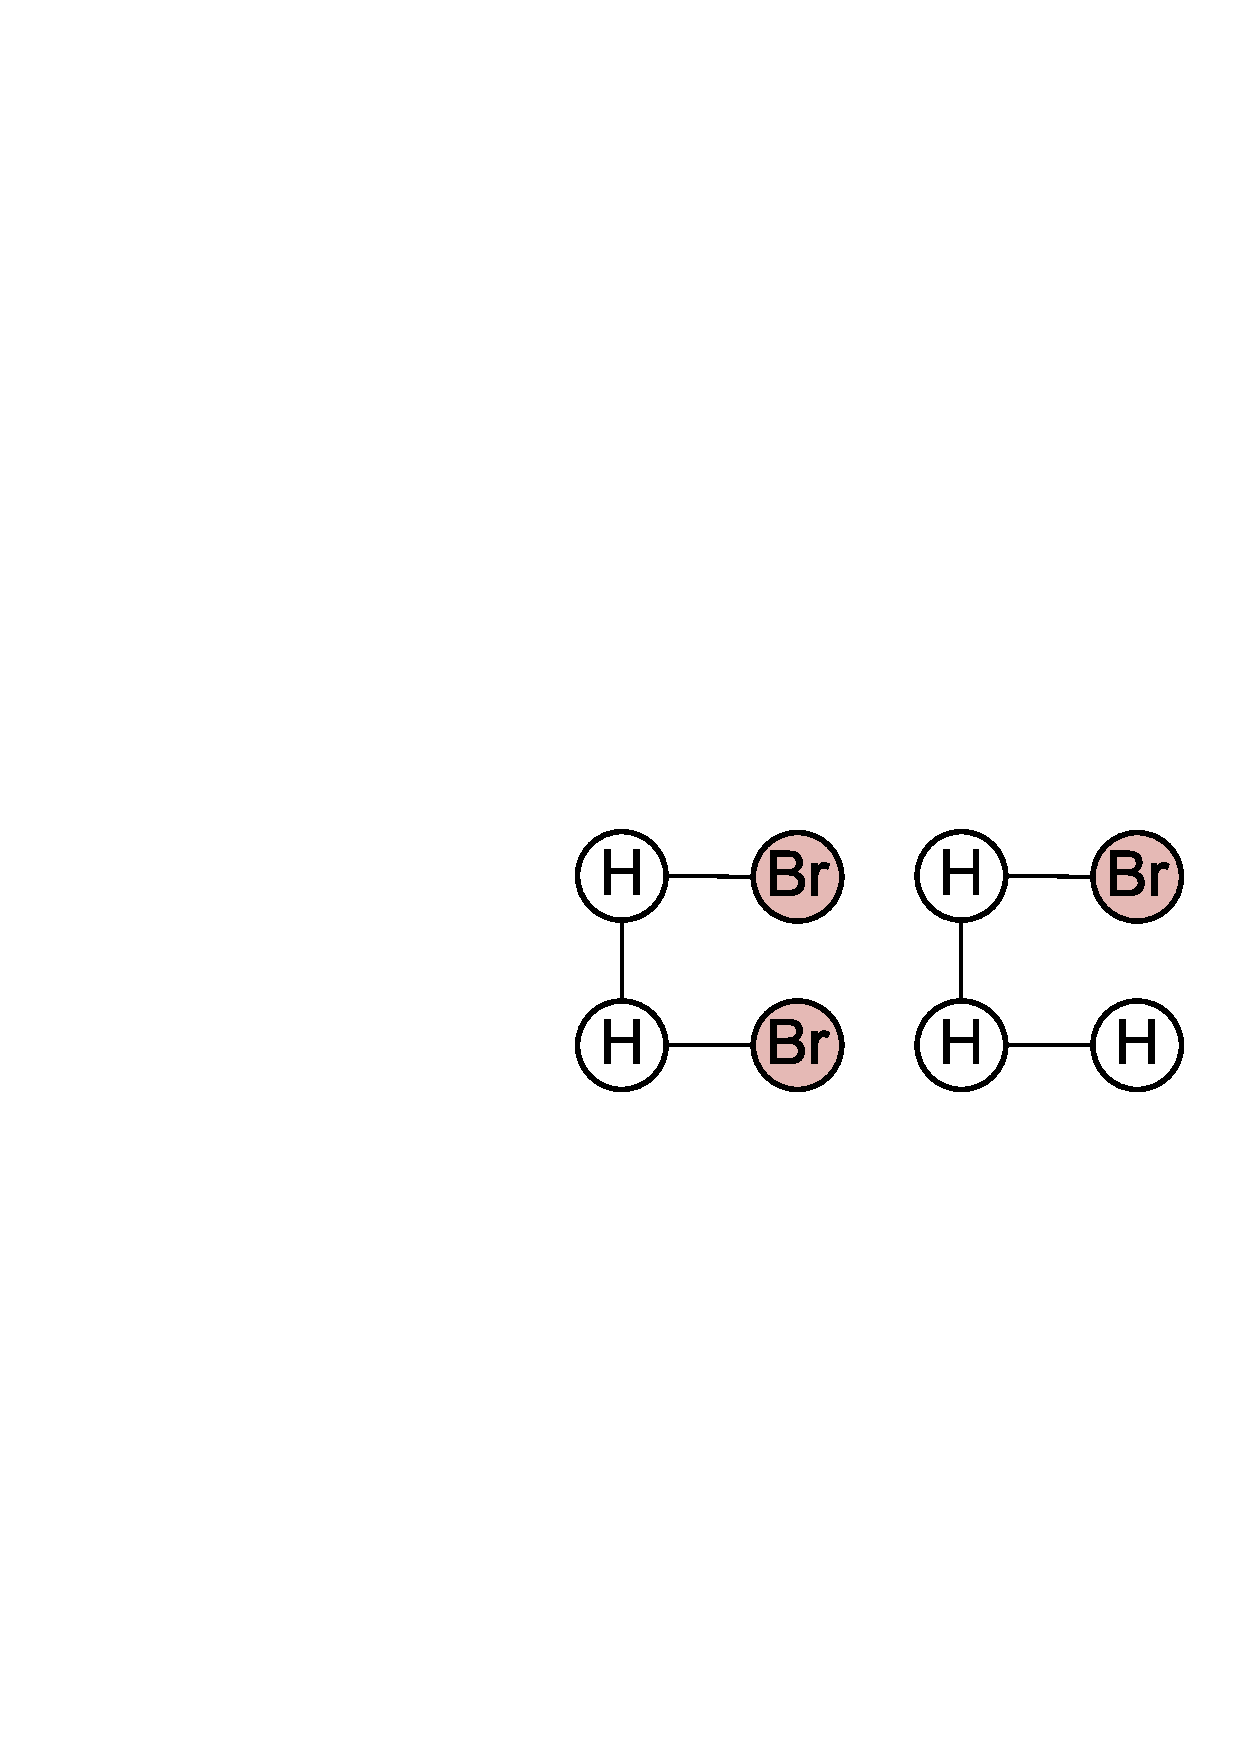
\includegraphics[scale=0.35]{images/result2}
% \label{fig:result2}
% }
% \vspace{-2mm}
% \caption{\scriptsize Figure for result analysis.}
% \label{fig:result}
% \vspace{-2mm}
% \end{figure}


% \par Also, we provide the {\sf Top-$3$} correlations of datasets {\em (1)(2)(3)(4)} in Figure \ref{fig:tp} and give an example for the analysis of some results. As in Figure \ref{fig:tp_lastfm}, the result shows that {\em Coldplay} is a popular band and people who like {\em Coldplay} are very likely to have some friends who like {\em Coldplay} as well. Besides, people who like {\em Radiohead} are very likely to be in the social group where many people like {\em Coldplay}.
% \par However, users may not be interested in some correlation like Figure \ref{fig:tp_dblp}. Due to its small size and symmetric structure, we can infer that if $h=1$, the subgraph pattern in Figure \ref{fig:result1} is very frequent. This job could already be done by frequent subgraph mining technique. Some users may also not interested in the correlation between just single edges. However, by simply limit the output correlation subgraph size, she can filter those small ones and reach her destination, like Figure \ref{fig:result2}.



% \spara{$\bullet$ vs. BFS \& DFS} We provide the comparison between best-first-search and the other two search strategies, BFS and DFS. In {\sf Top-$k$} mining, best-first-strategy outperforms both BFS and DFS apparently. In {\sf Min-sup} mining, all of the 3 strategies have the similar performances in time efficiency. Besides, since the space cost of our algorithm is dominated by the distance index so that the 3 strategies also have a similar space consumption.


% \begin{figure}[t!]
% \vspace{4mm}
% \centering
% \subfigure[{\scriptsize {\em DBLP} with {\sf Min-sup} = $5000$, $h=2$}] {
% 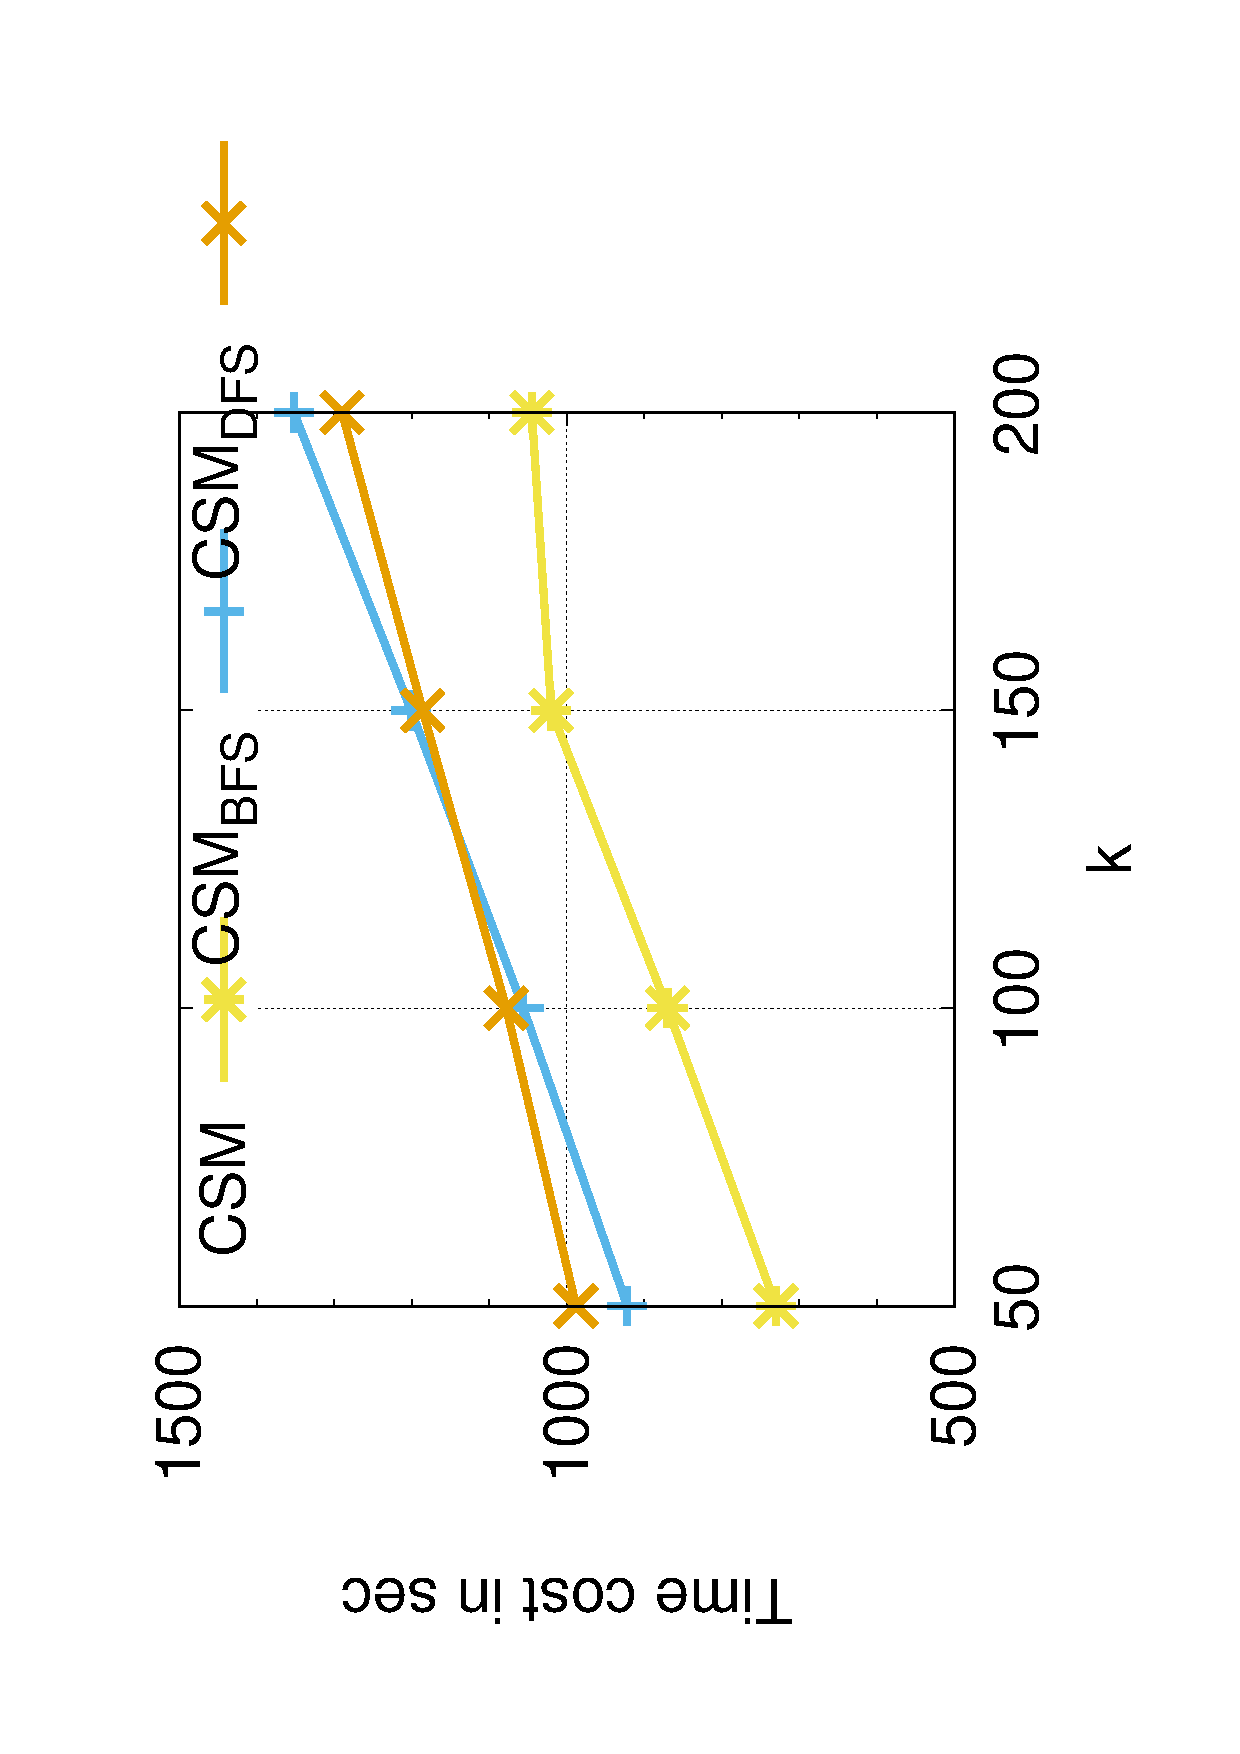
\includegraphics[scale=0.17, angle=270]{addimg/dbfs_dblp}
% \label{fig:dbfs1}
% }
% \subfigure[{\scriptsize {\em LastFM} with {\sf Min-sup} = $200$, $h=2$}]  {
% 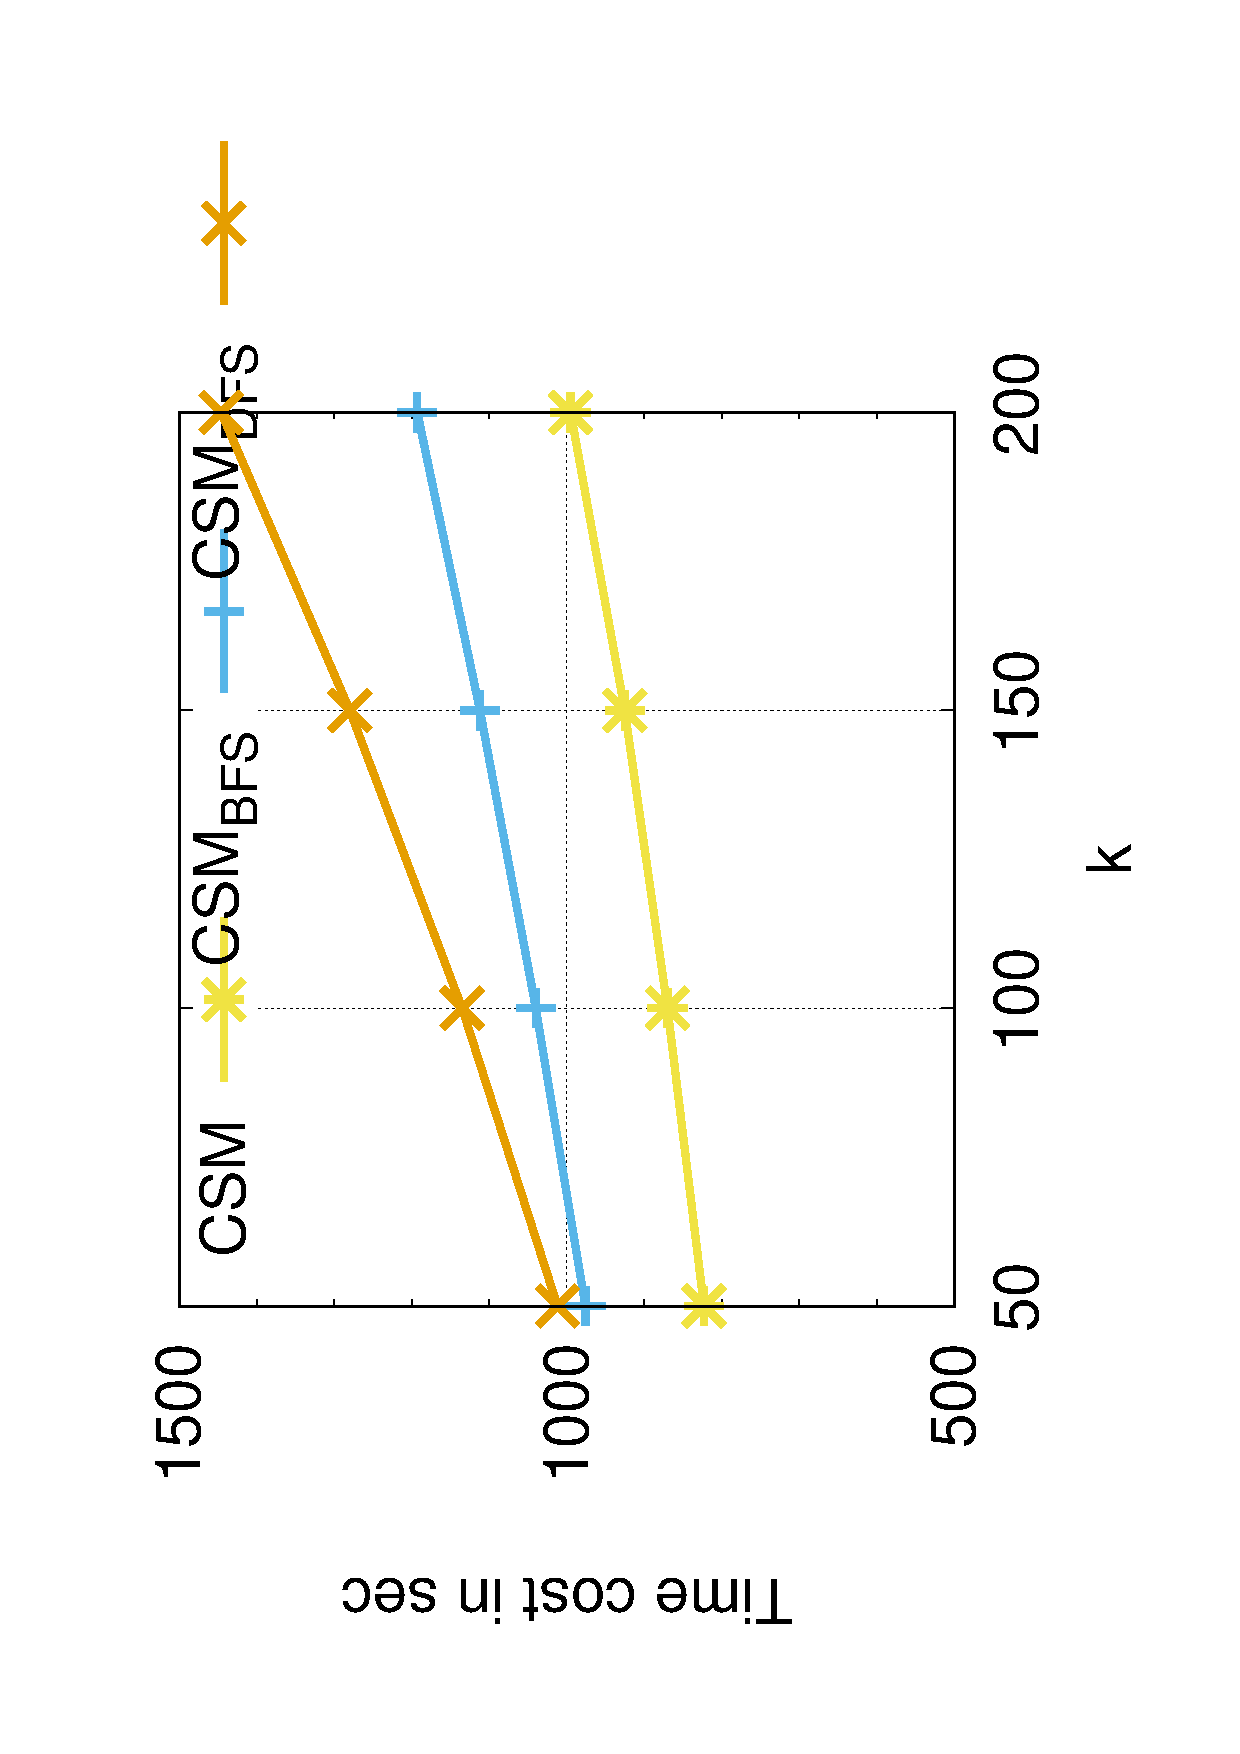
\includegraphics[scale=0.17, angle=270]{addimg/dbfs_lastfm}
% \label{fig:dbfs2}
% }
% \vspace{-2mm}
% \caption{\scriptsize Comparison with BFS and DFS.}
% \label{fig:dbfs}
% \vspace{-2mm}
% \end{figure}


% \spara{$\bullet$ Index Analysis} We provide the result of efficiency increase of our global index. The index strategy is more powerful if there are fewer distinct edge labels or the data graph is more dense, like {\em Yeast} and {\em DBLP}.


% \begin{figure}[t!]
% \vspace{4mm}
% \centering
% \subfigure[{\scriptsize {\em Chemical} with {\sf Min-sup} = $10$, $k=50$}] {
% 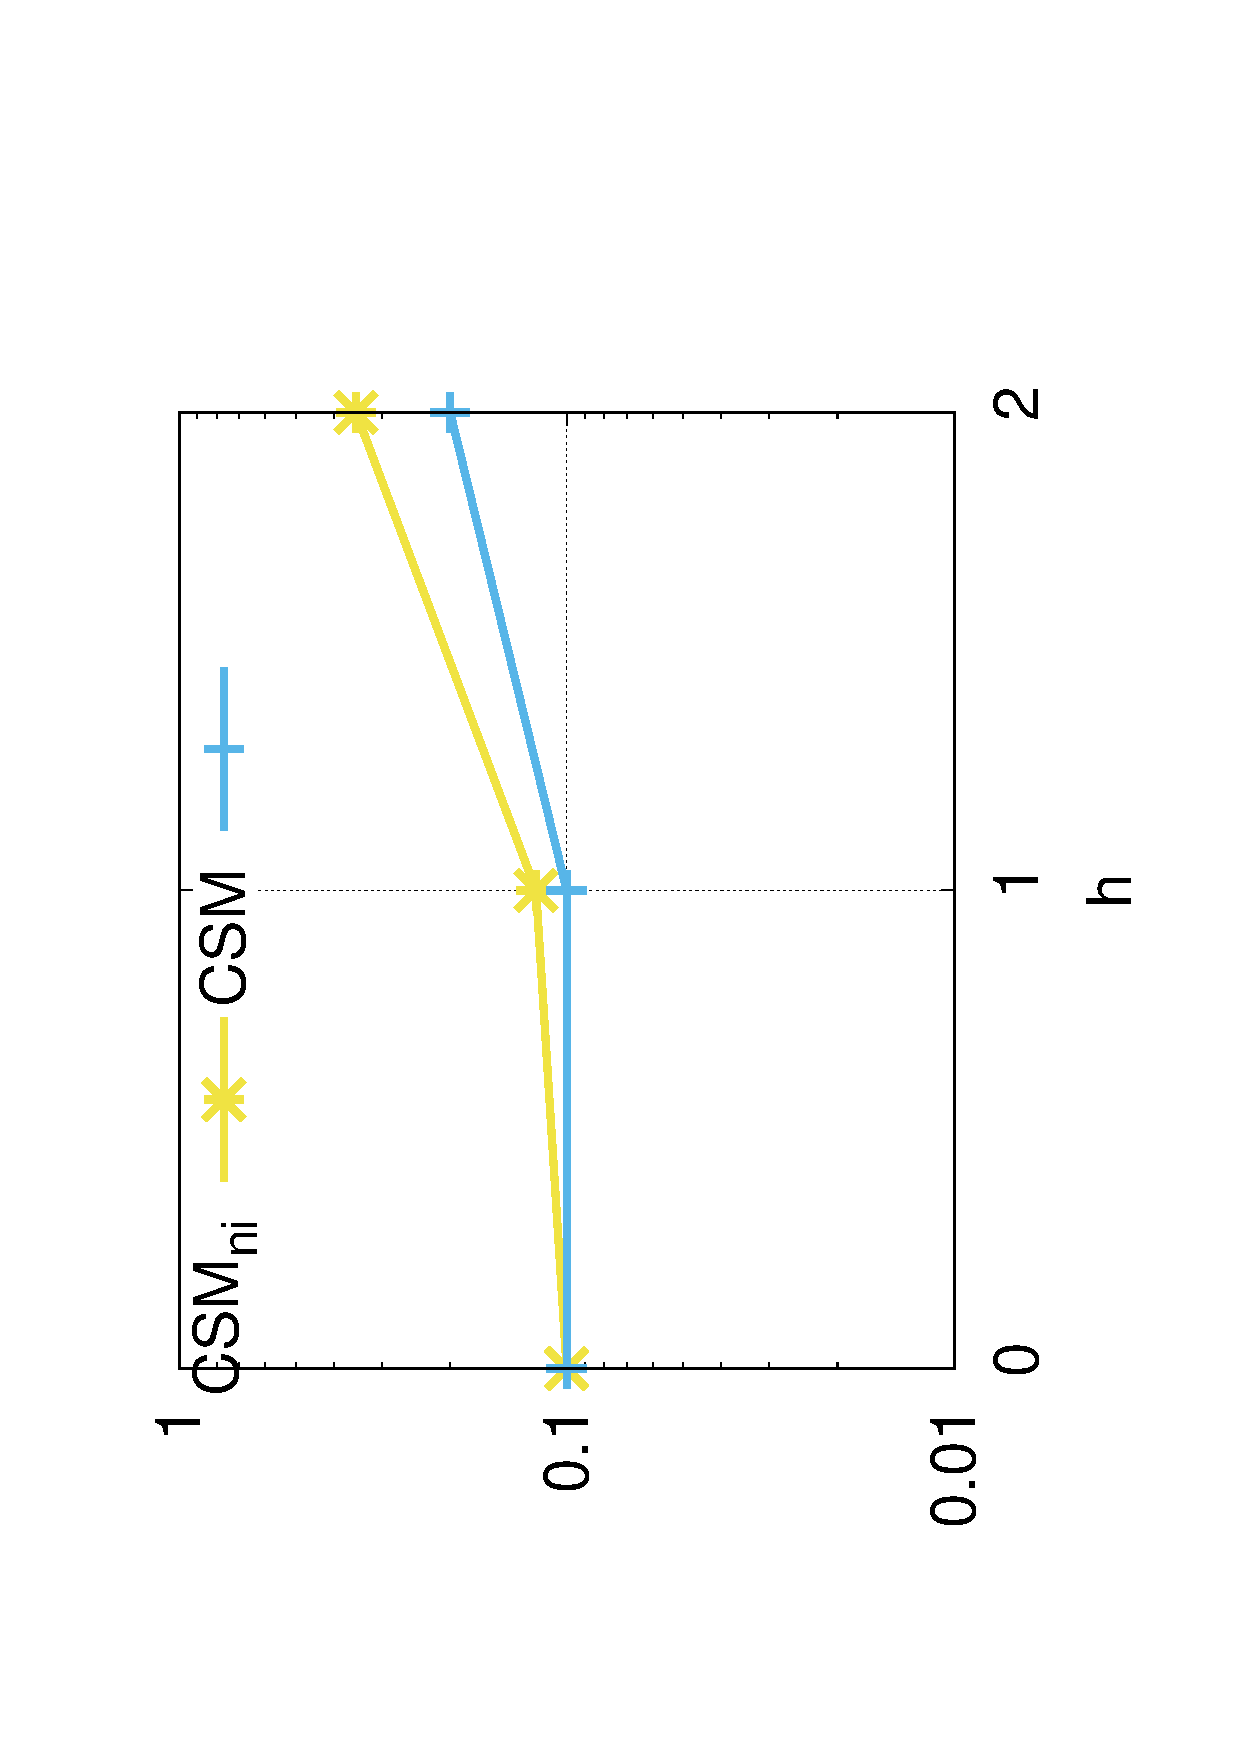
\includegraphics[scale=0.17, angle=270]{img2/ni_chemical}
% \label{fig:ni1}
% }
% \subfigure[{\scriptsize {\em Yeast} with {\sf Min-sup} = $200$, $k=50$}]  {
% 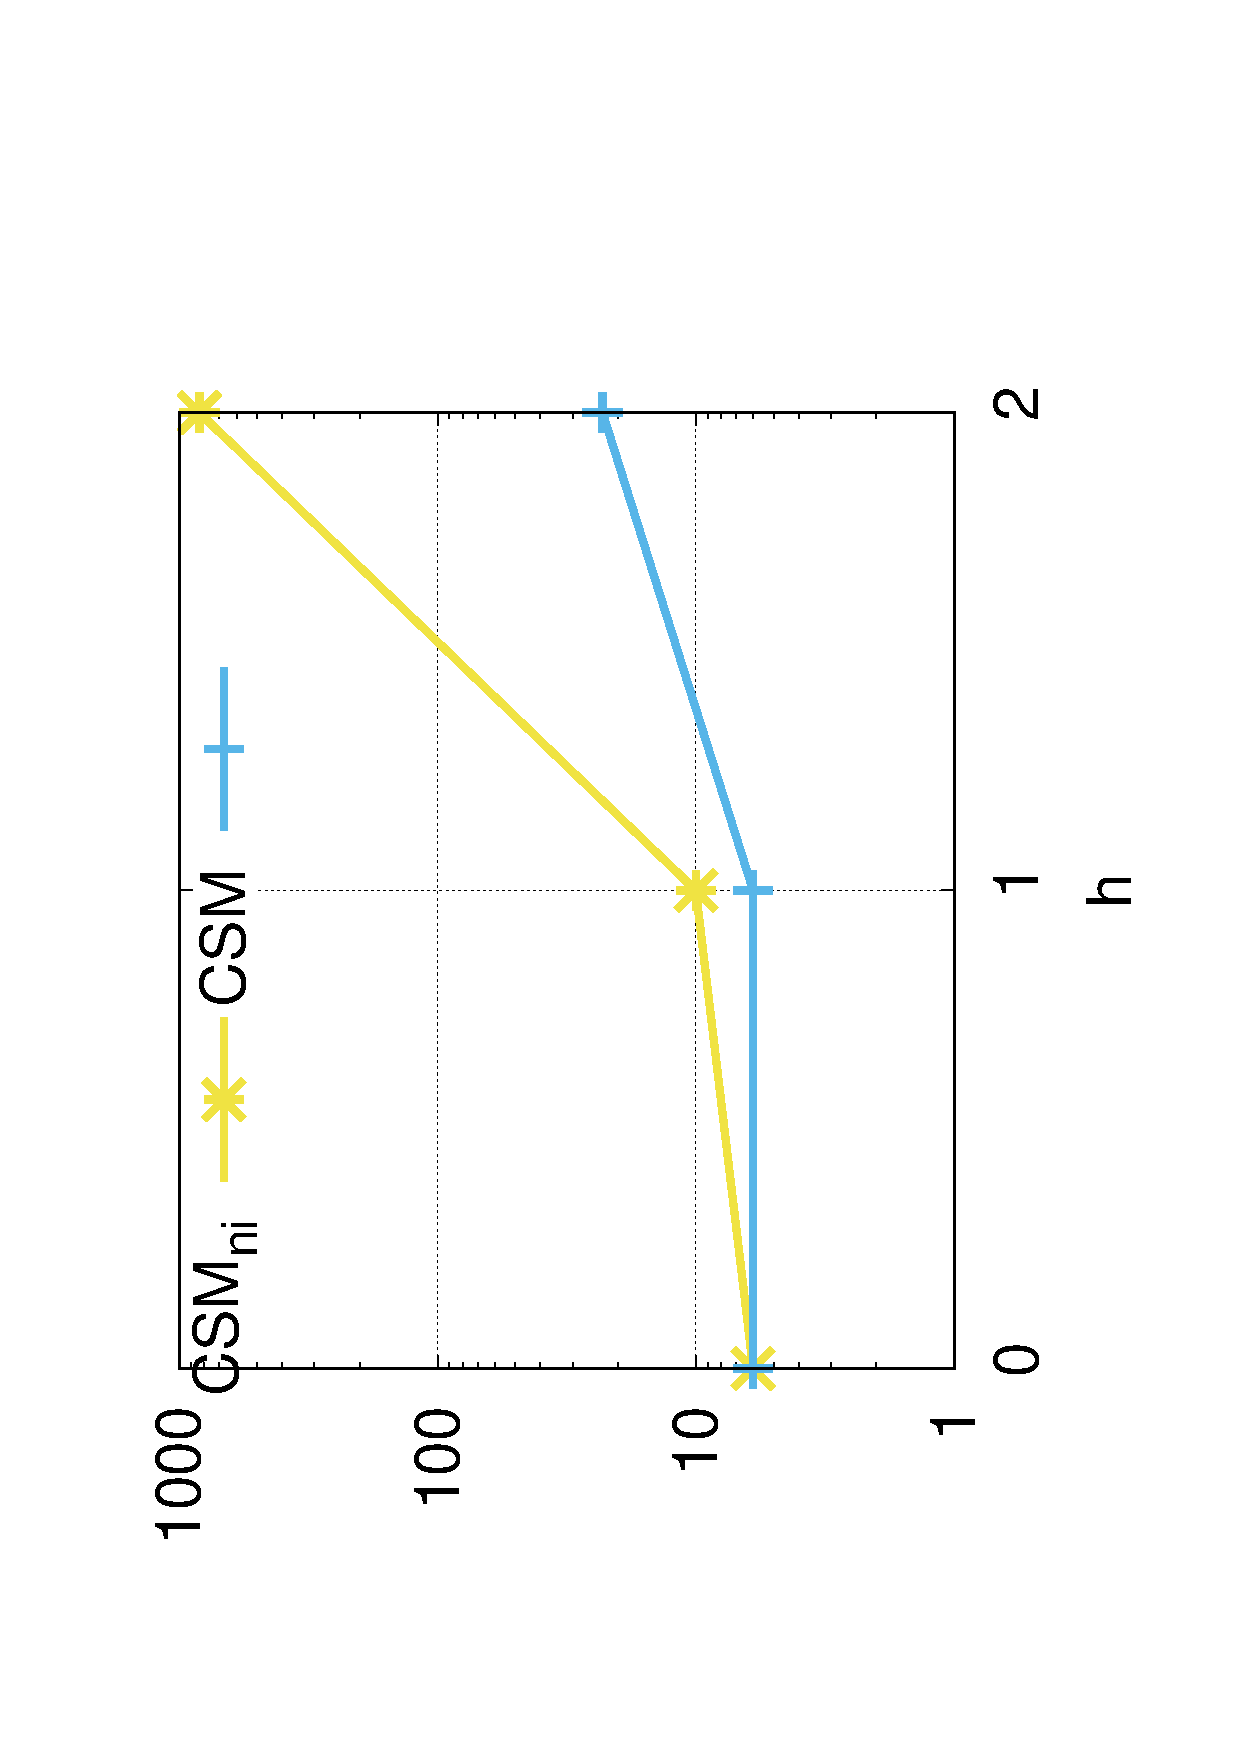
\includegraphics[scale=0.17, angle=270]{img2/ni_yeast}
% \label{fig:ni2}
% }
% \subfigure[{\scriptsize {\em DBLP} with {\sf Min-sup} = $5000$, $k=50$}] {
% 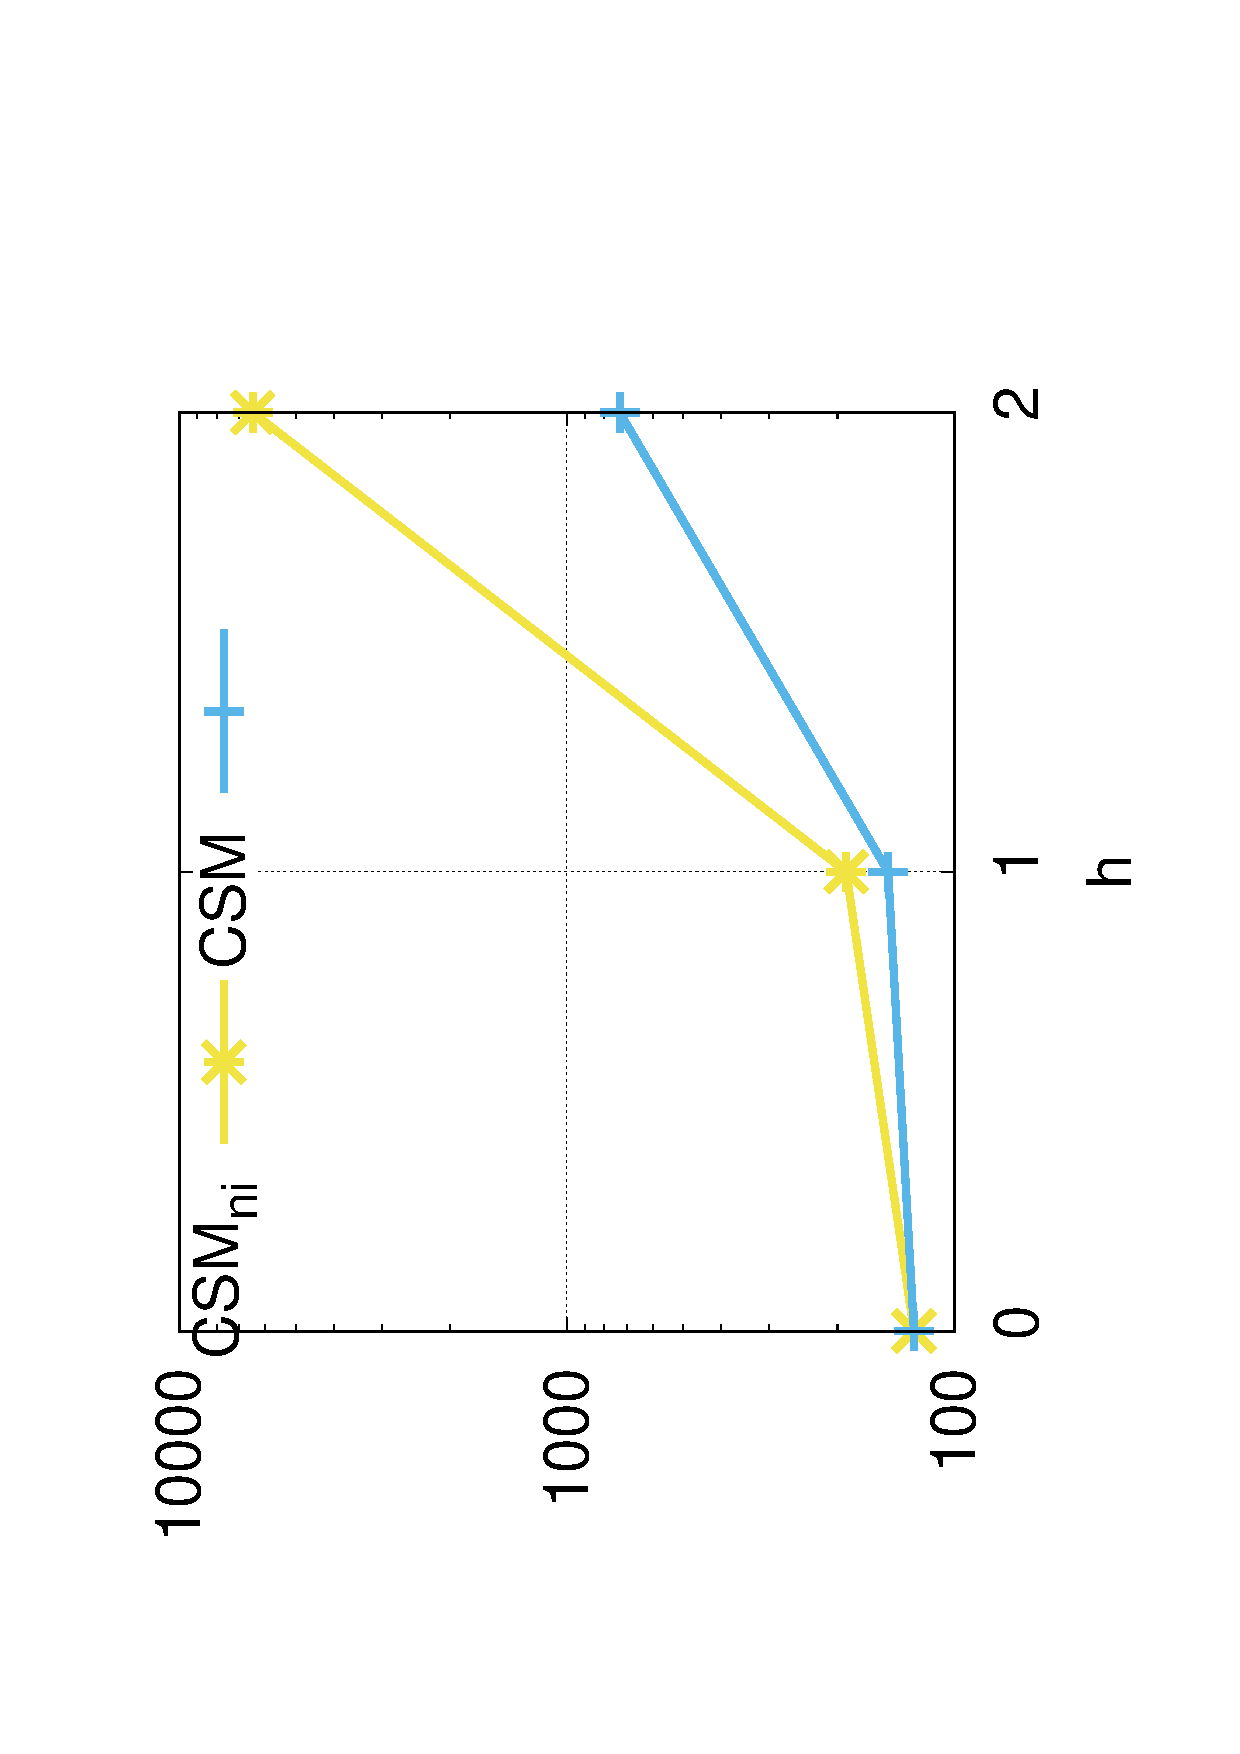
\includegraphics[scale=0.17, angle=270]{img2/ni_dblp}
% \label{fig:ni3}
% }
% \subfigure[{\scriptsize {\em LastFM} with {\sf Min-sup} = $200$, $k=50$}]  {
% 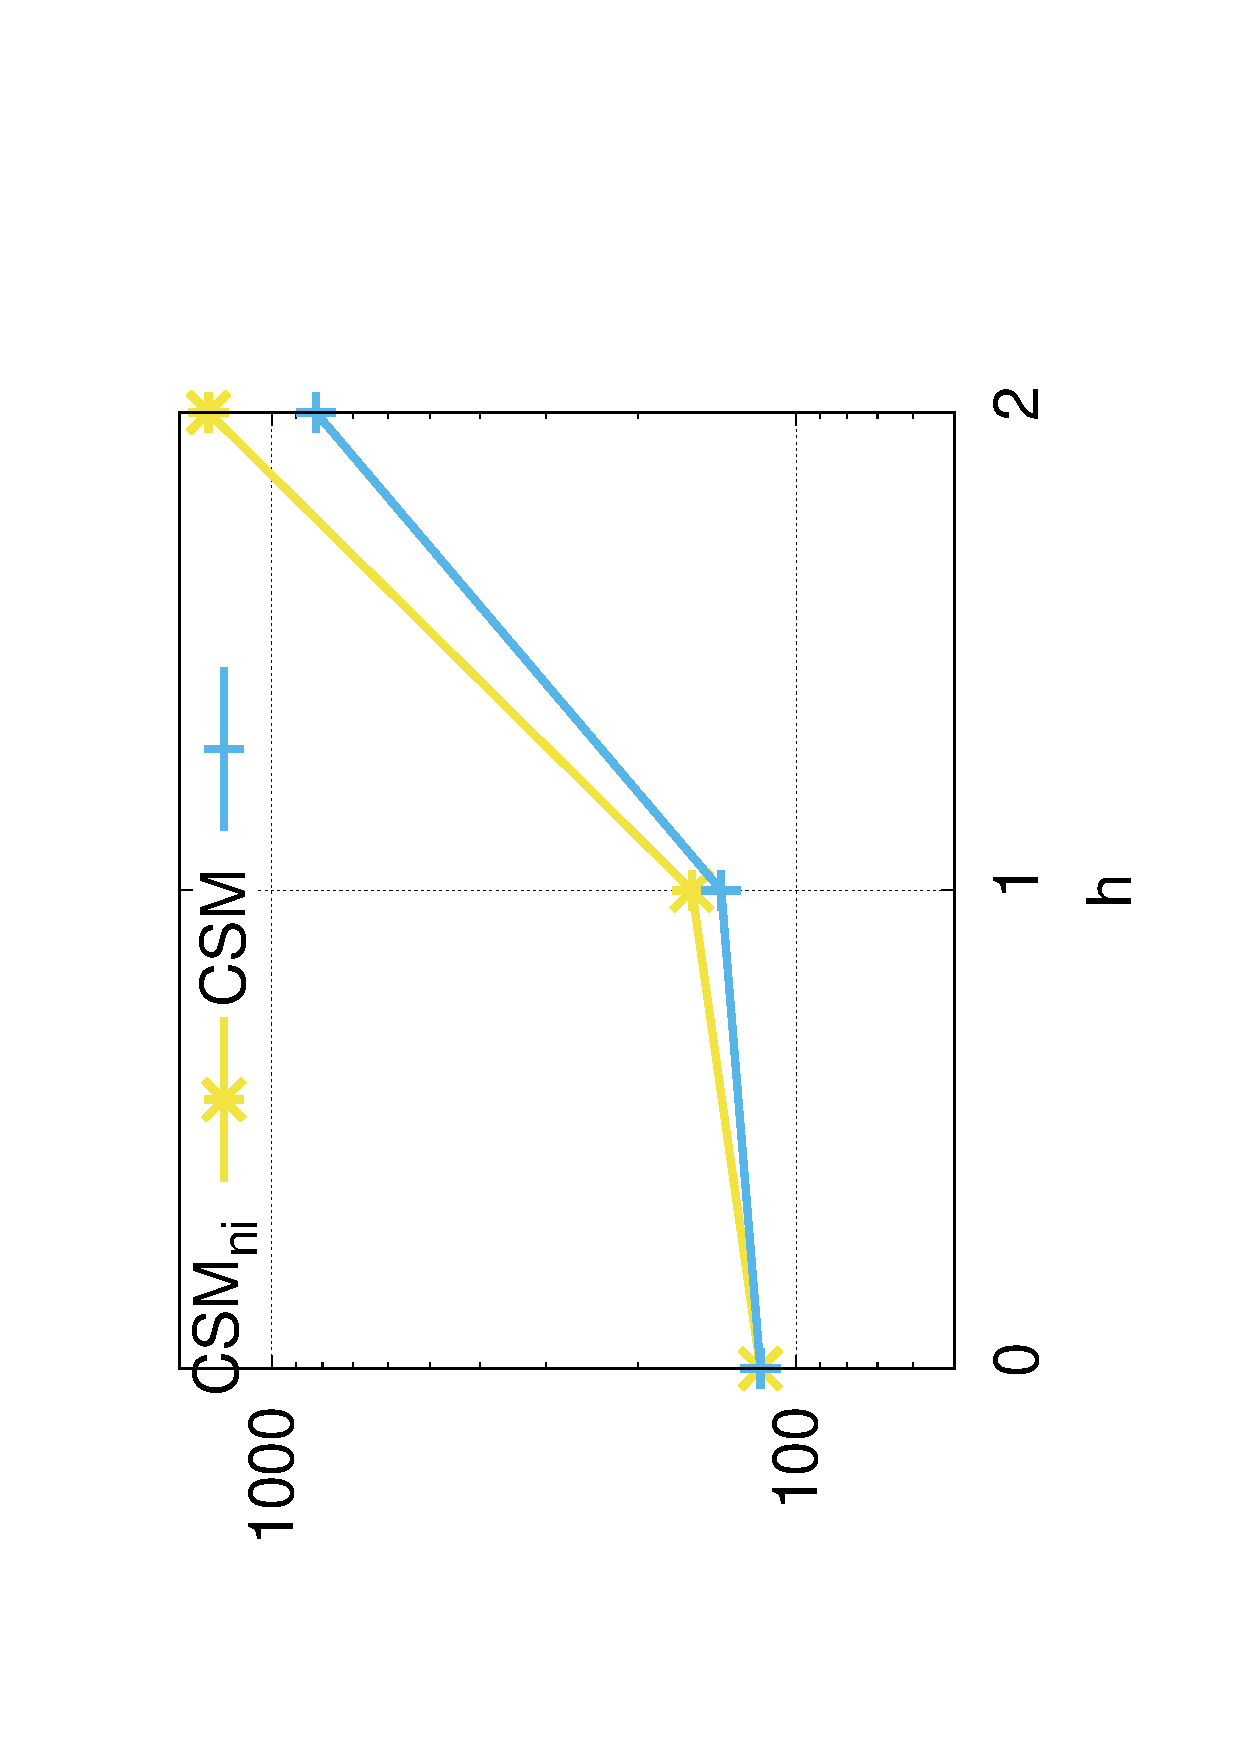
\includegraphics[scale=0.17, angle=270]{img2/ni_lastfm}
% \label{fig:ni4}
% }
% \vspace{-2mm}
% \caption{\scriptsize Figure for index analysis.}
% \label{fig:ni}
% \vspace{-2mm}
% \end{figure}



% \spara{$\bullet$ Further Analysis} We provide some further analysis. This part contains the result of the optimization of changing collection tree root in Section \ref{subsubsec:recursive}, and the time cost we spend to avoid the subgraph/supergraph correlations. According to the experimental result, the time we use to prune the not interesting correlations is about 10\% of the total time. Besides, the root changing optimization in Section \ref{subsubsec:recursive} increase the time efficiency by 10\%.


% \begin{figure}[t!]
% \vspace{4mm}
% \centering
% \subfigure[{\scriptsize {\em DBLP} with {\sf Min-sup} = $5000$, $h=2$}] {
% 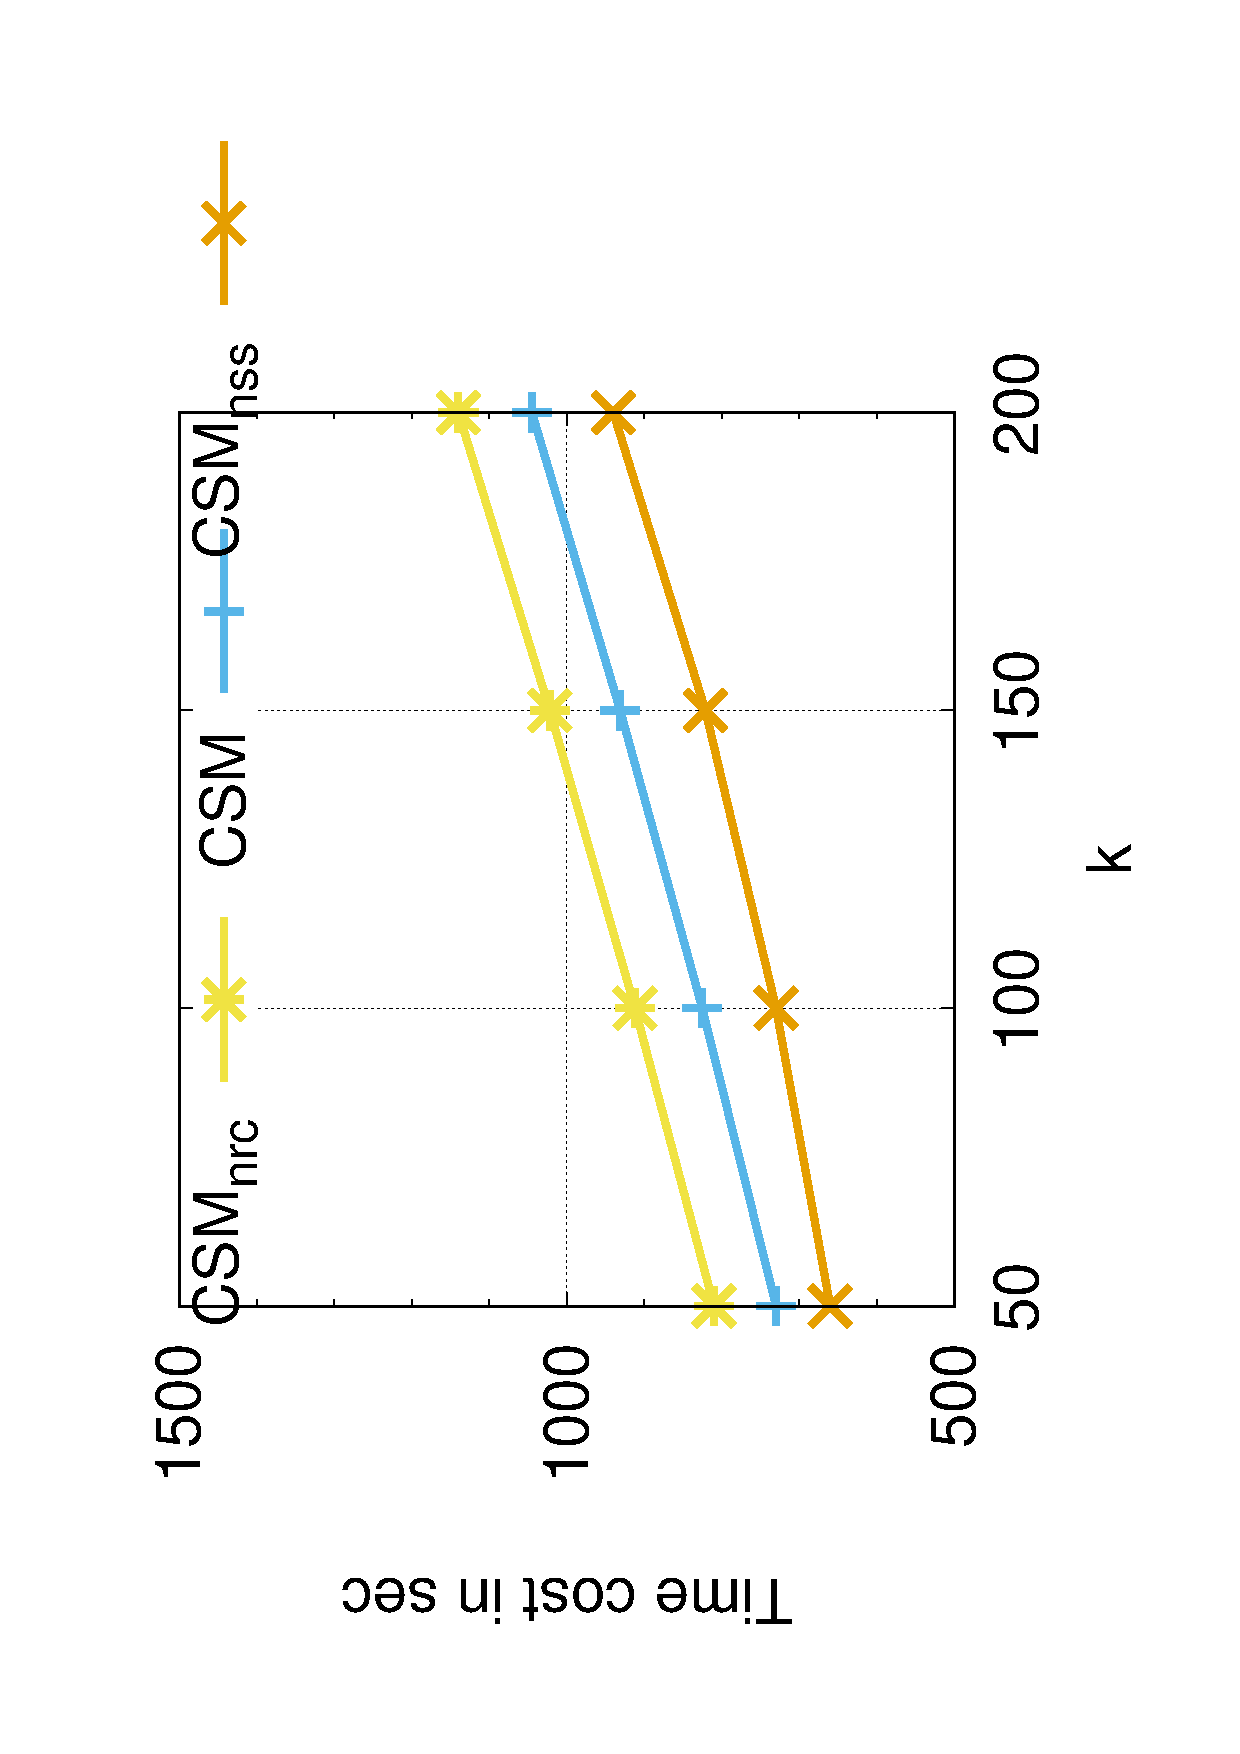
\includegraphics[scale=0.17, angle=270]{addimg/opt_dblp}
% \label{fig:opt1}
% }
% \subfigure[{\scriptsize {\em LastFM} with {\sf Min-sup} = $200$, $h=2$}]  {
% 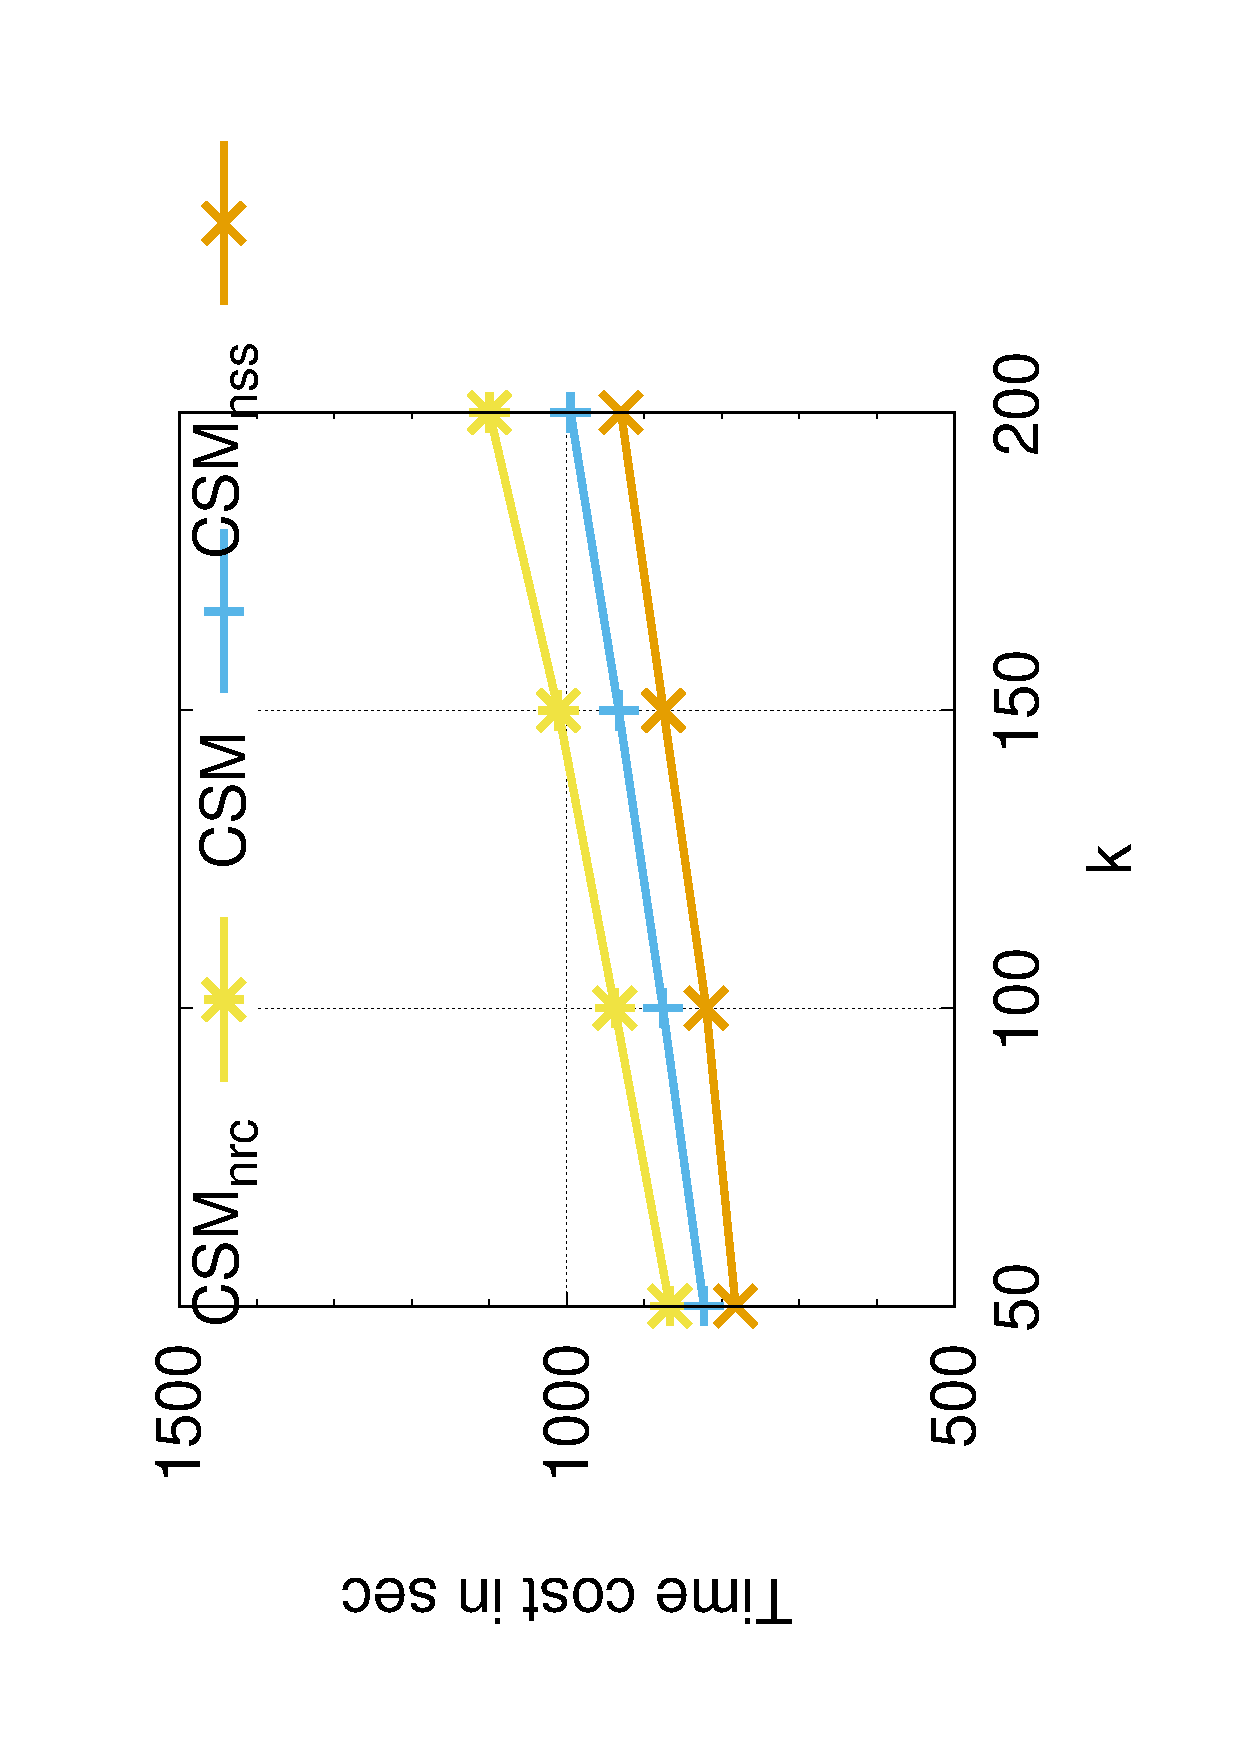
\includegraphics[scale=0.17, angle=270]{addimg/opt_lastfm}
% \label{fig:opt2}
% }
% \vspace{-2mm}
% \caption{\scriptsize Figure for further analysis.}
% \label{fig:opt}
% \vspace{-2mm}
% \end{figure}


% \spara{$\bullet$ Approximation Algorithm Analysis.} We provide the experimental result of our approximation mining algorithm.


% \begin{figure}[t!]
% \vspace{4mm}
% \centering
% \subfigure[{\scriptsize {\em DBLP} with {\sf Min-sup} = $5000$}] {
% 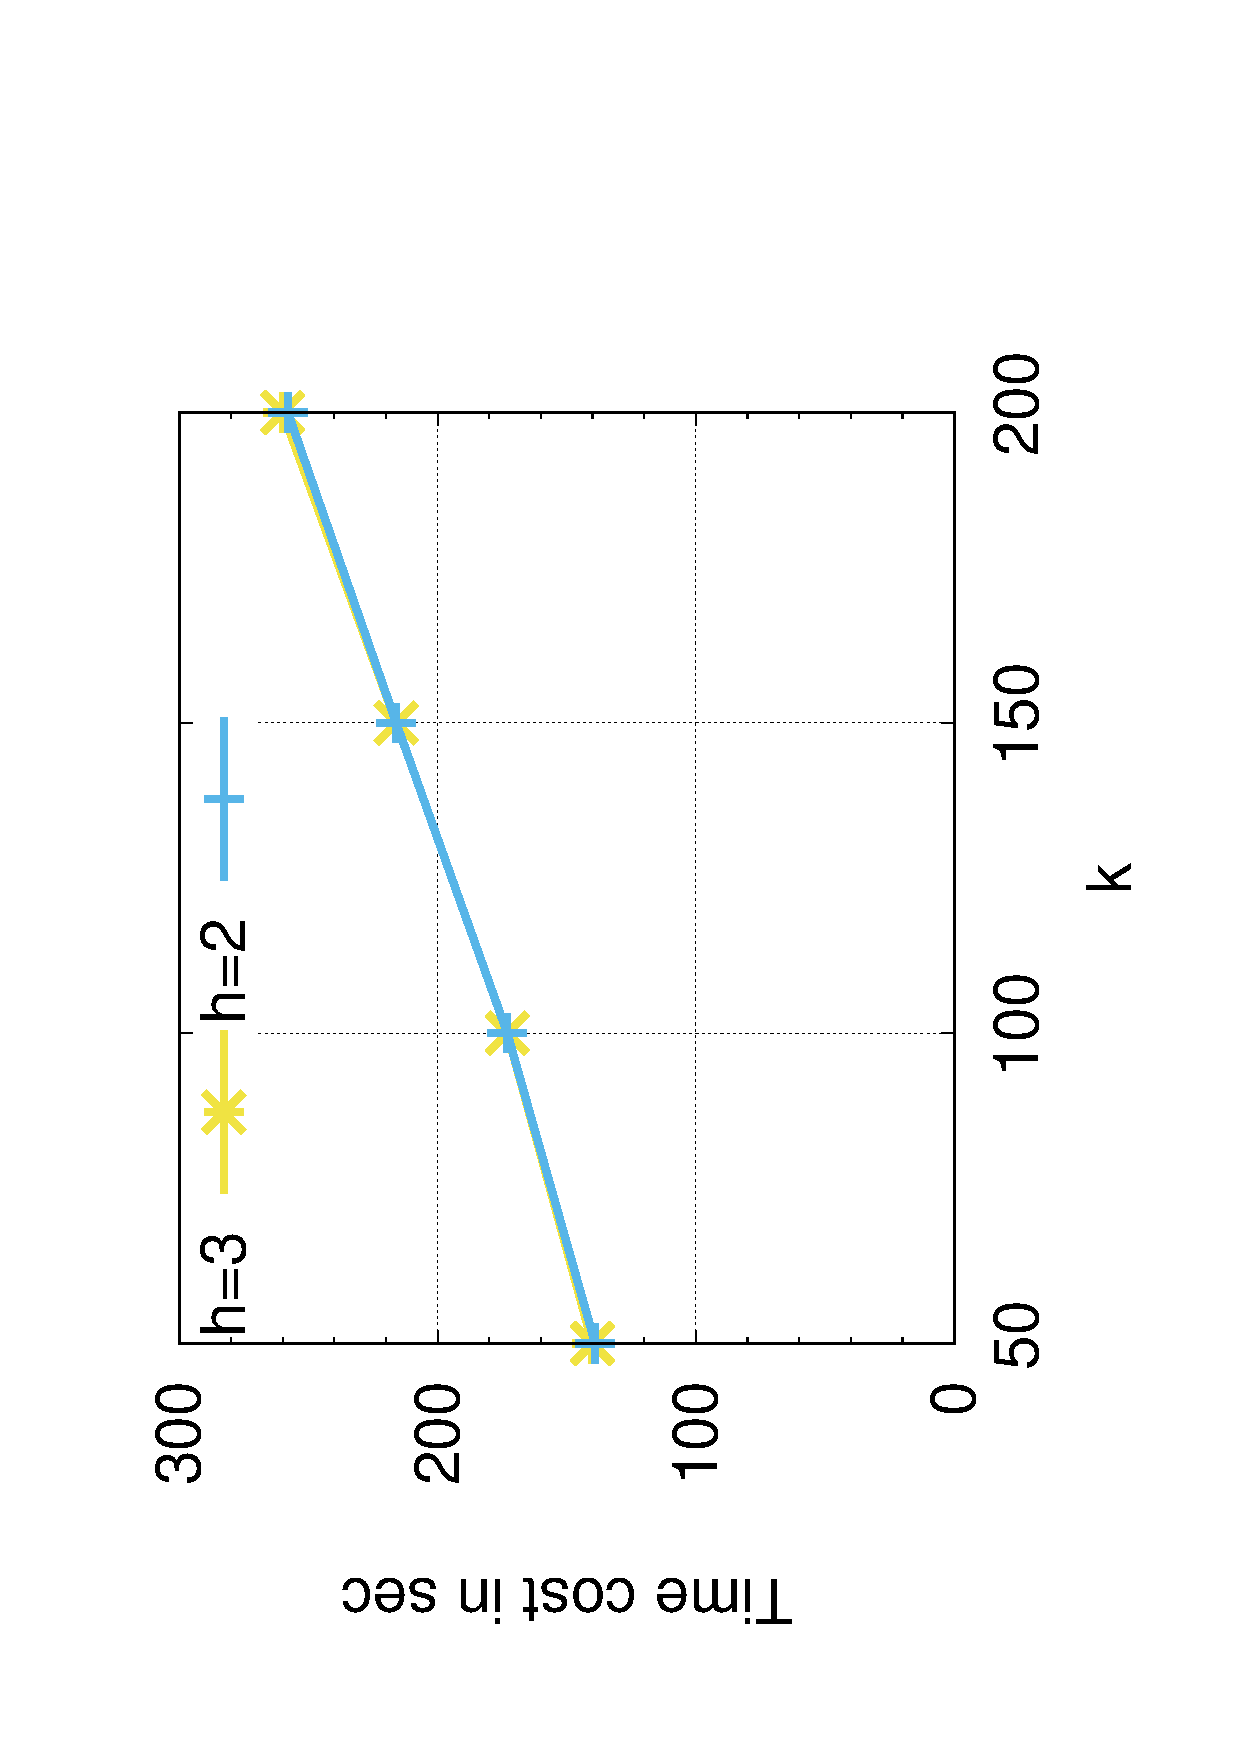
\includegraphics[scale=0.17, angle=270]{addimg/a_dblp}
% \label{fig:ap1}
% }
% \subfigure[{\scriptsize {\em LastFM} with {\sf Min-sup} = $200$}]  {
% 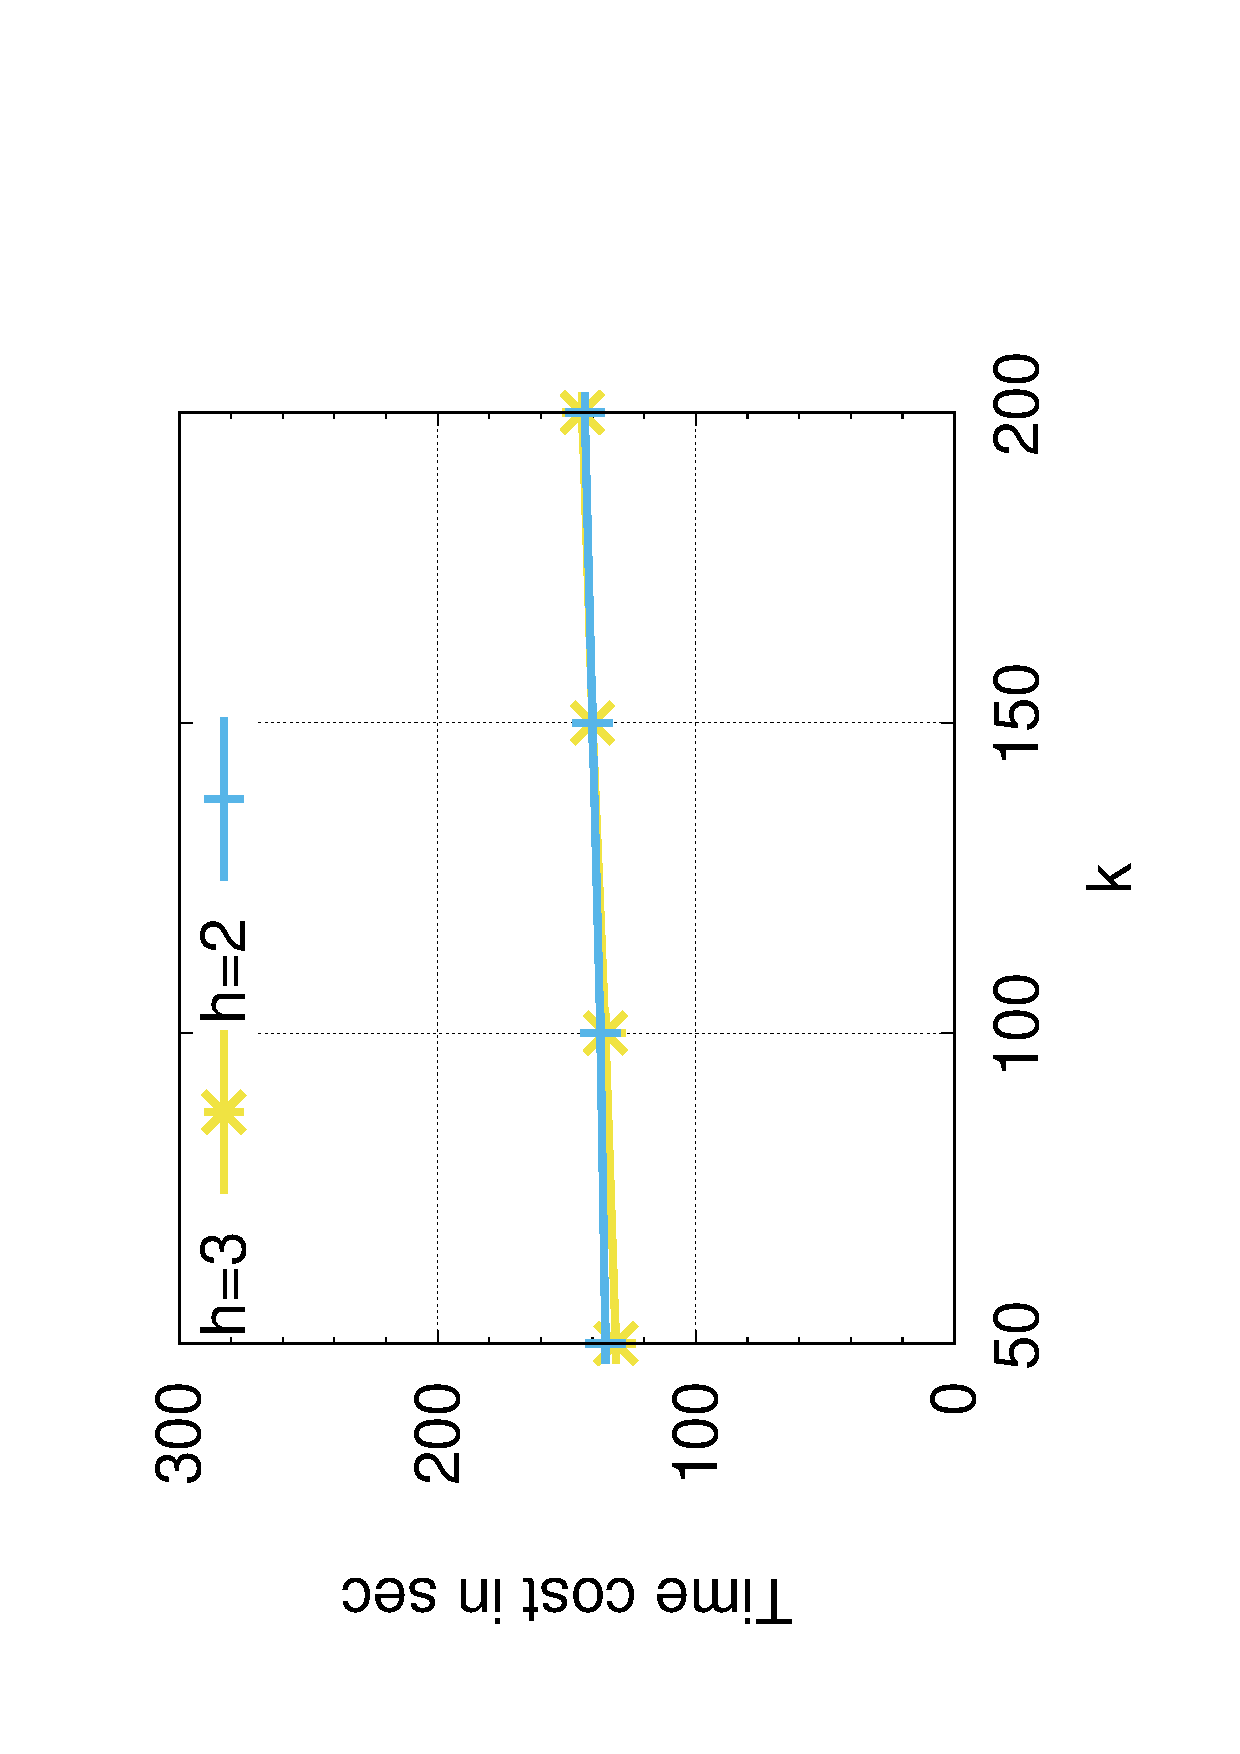
\includegraphics[scale=0.17, angle=270]{addimg/a_lastfm}
% \label{fig:ap2}
% }
% \vspace{-2mm}
% \caption{\scriptsize Figure for approximation algorithm analysis.}
% \label{fig:ap}
% \vspace{-2mm}
% \end{figure}



% \begin{figure}[t!]
% \vspace{-2mm}
% \centering
% \subfigure[{\scriptsize FSM on {\em Chemical}}] {
% 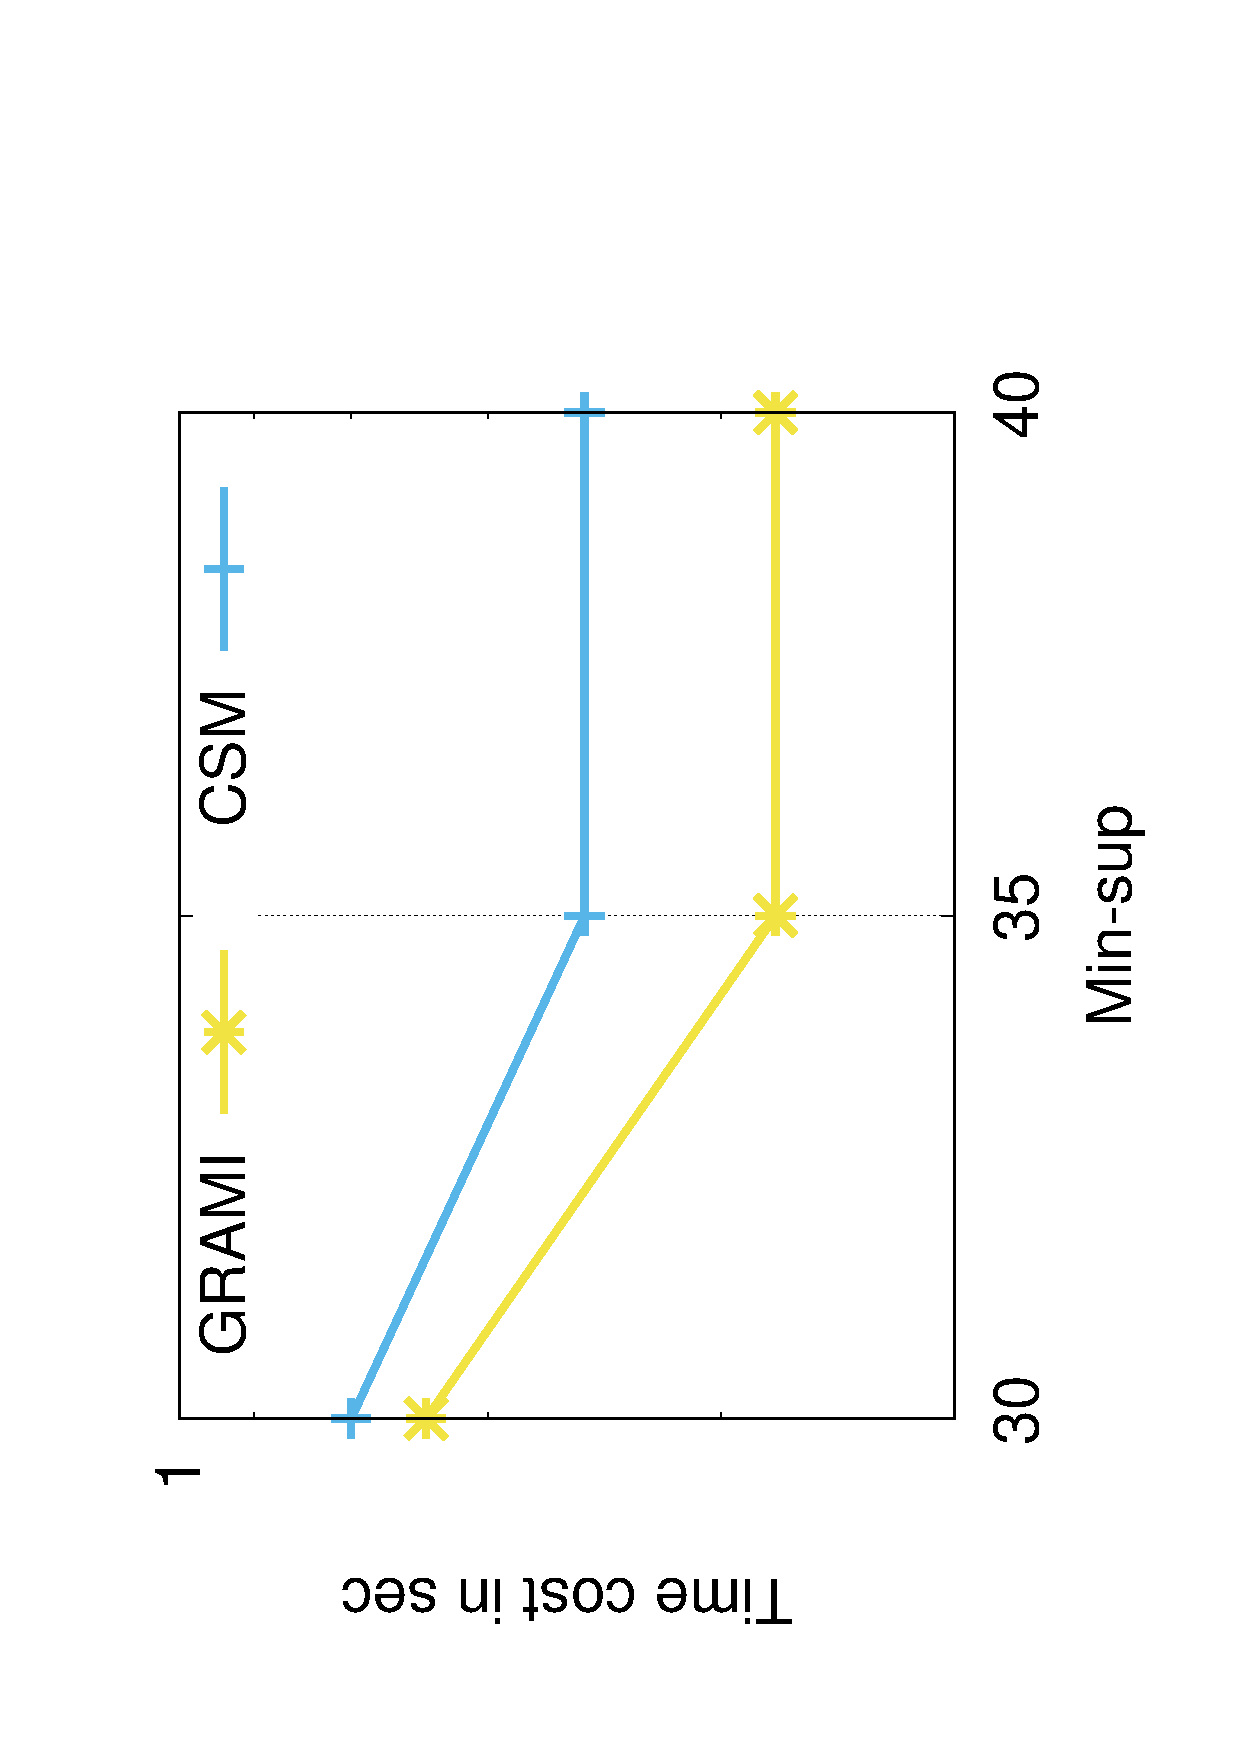
\includegraphics[scale=0.17, angle=270]{img2/fsm_chemical}
% \label{fig:grami1}
% }
% \subfigure[{\scriptsize FSM on {\em Yeast}}]  {
% 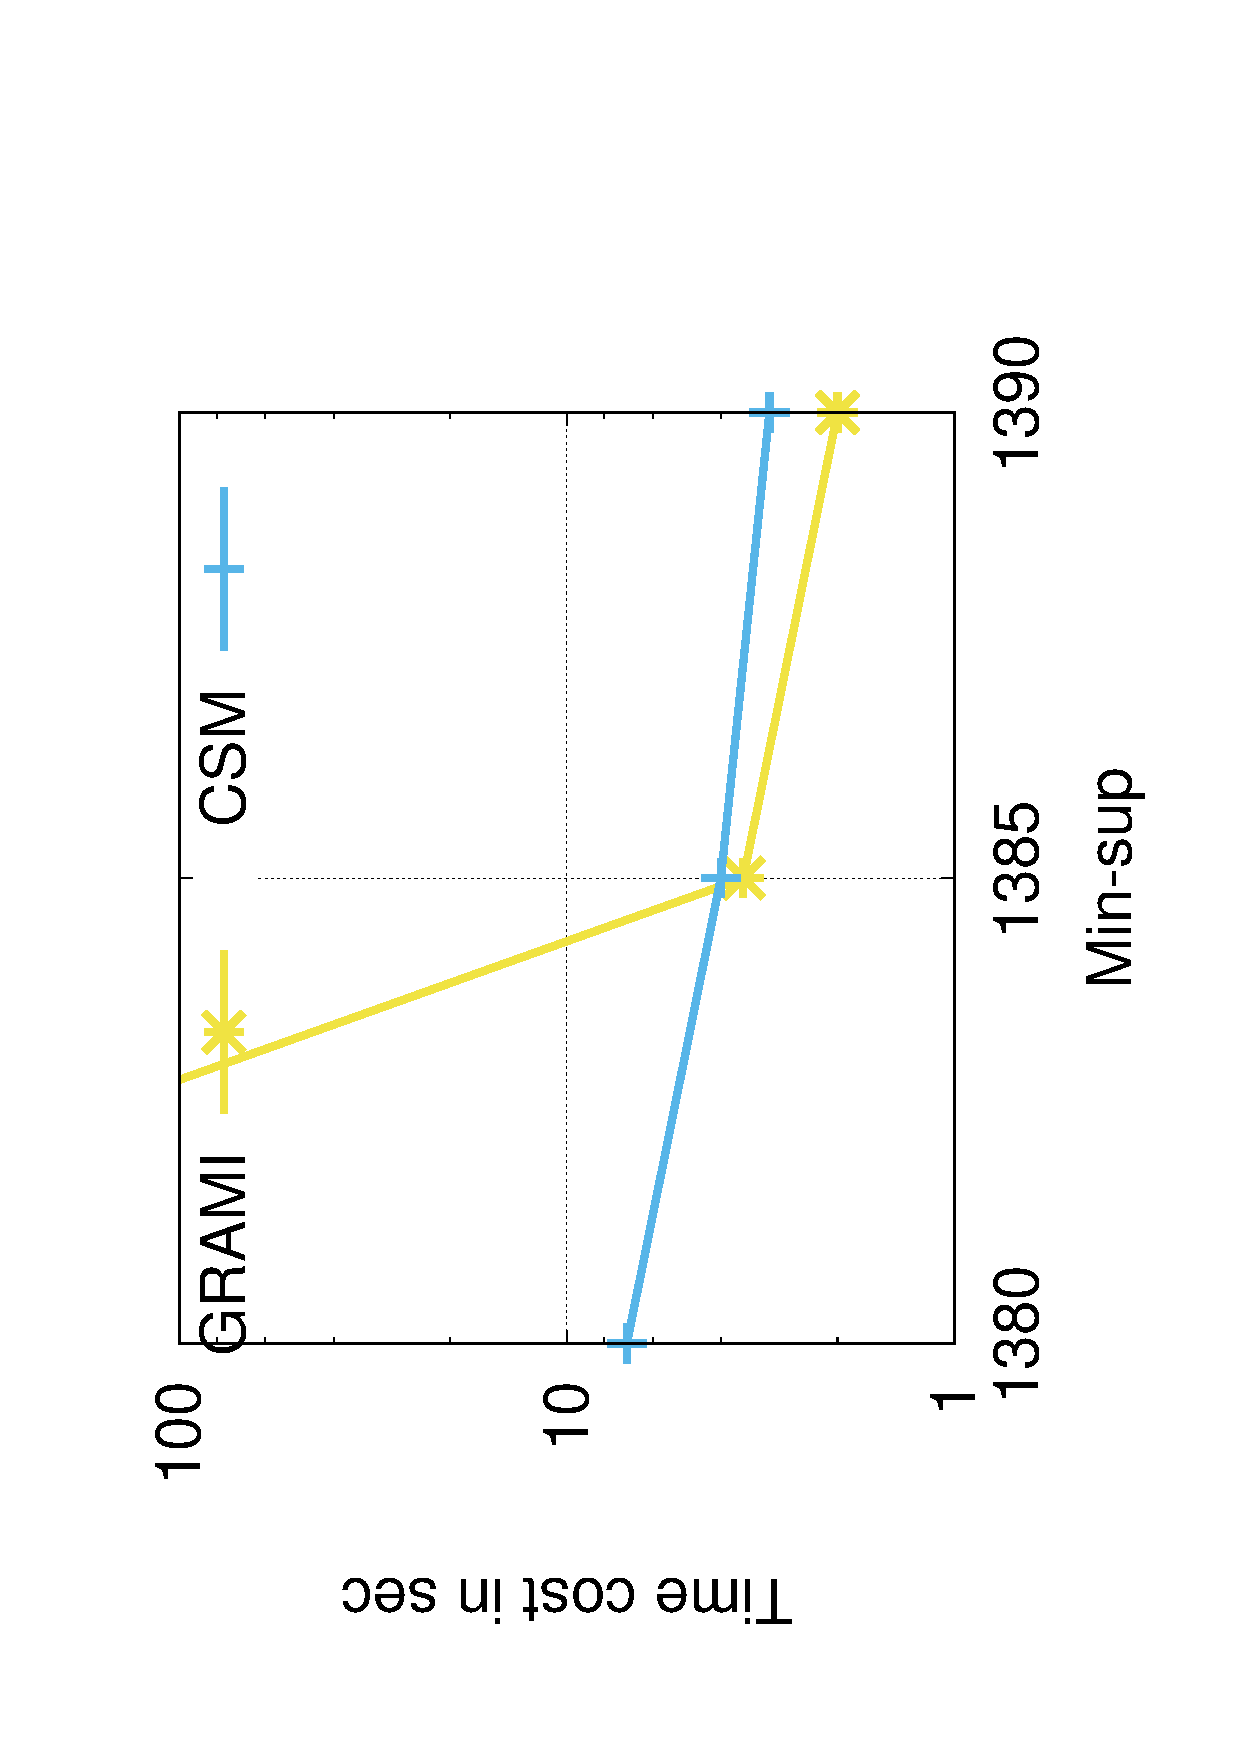
\includegraphics[scale=0.17, angle=270]{img2/fsm_yeast}
% \label{fig:grami2}
% }
% \subfigure[{\scriptsize FSM on {\em DBLP}}] {
% 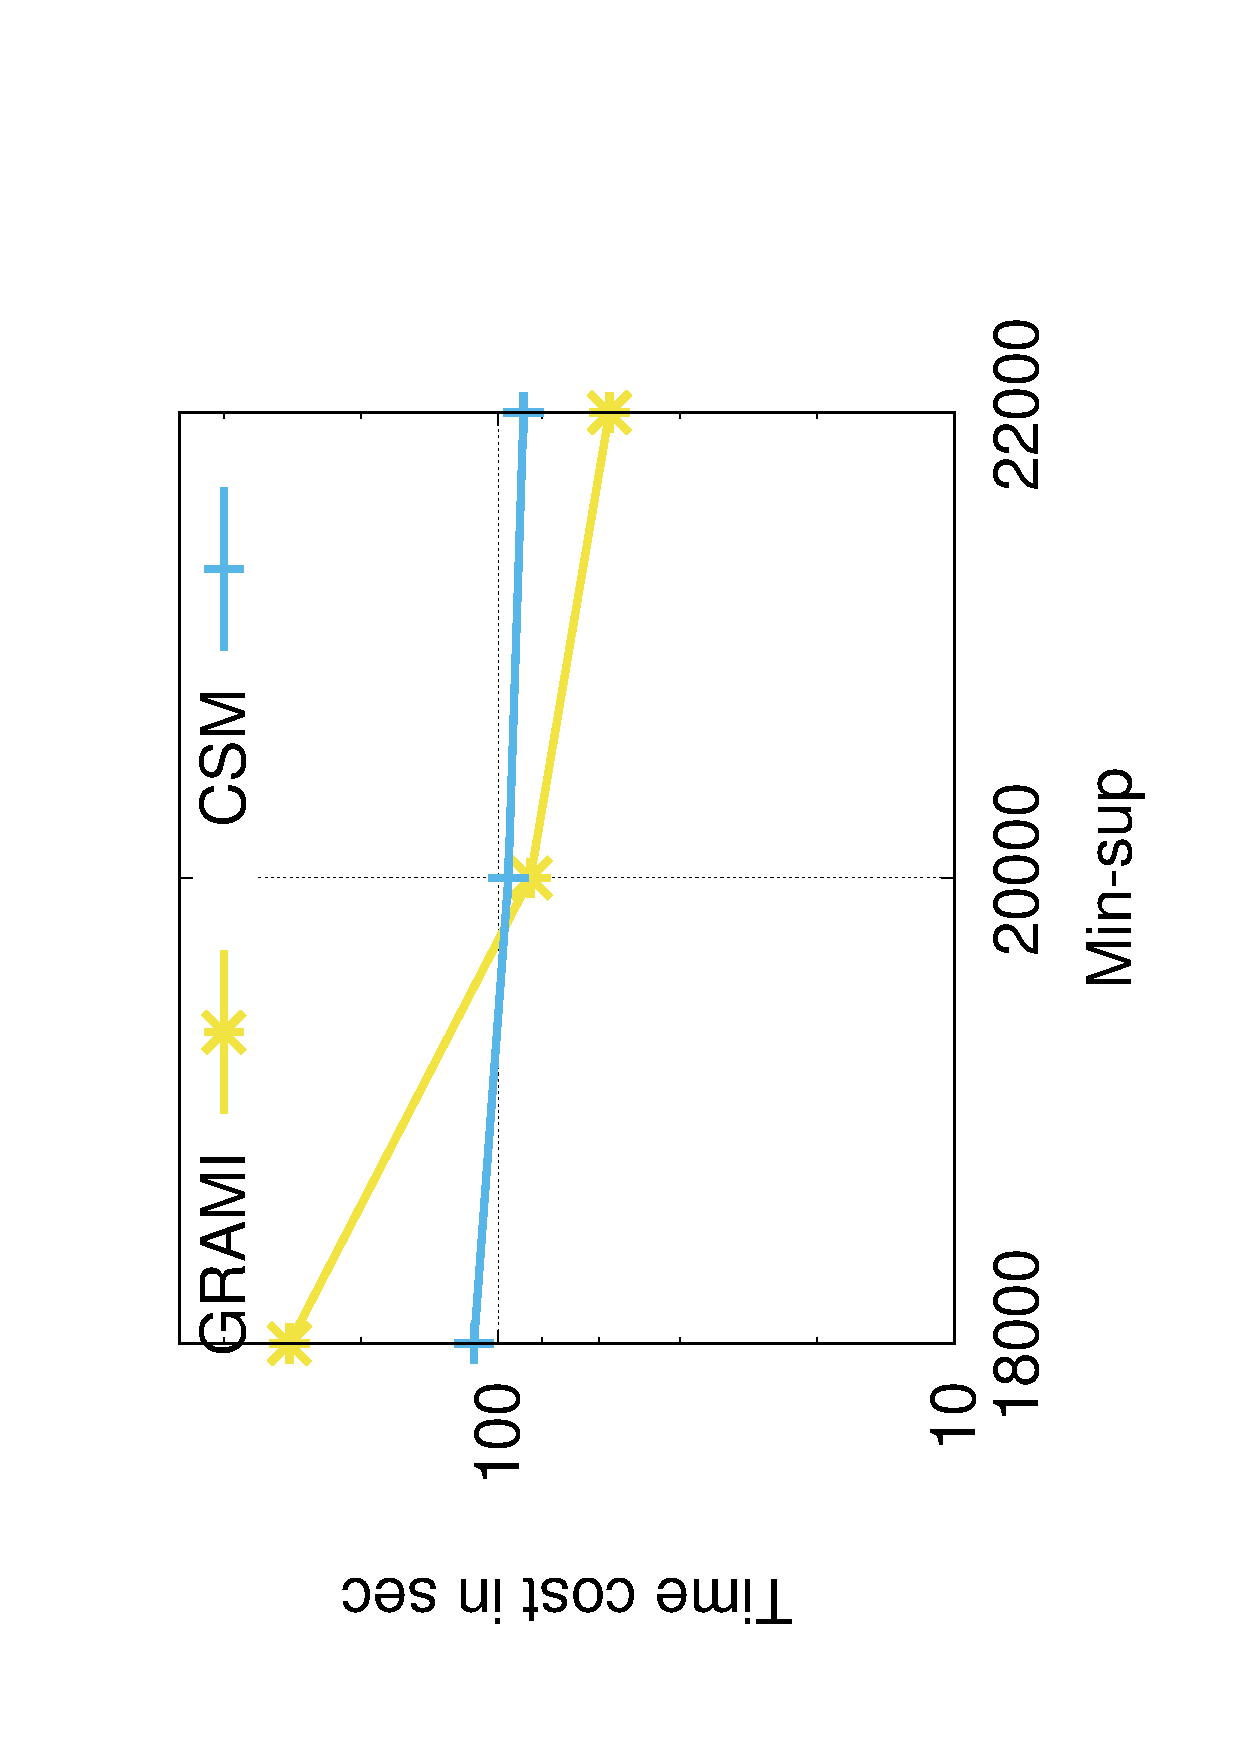
\includegraphics[scale=0.17, angle=270]{img2/fsm_dblp}
% \label{fig:grami3}
% }
% \subfigure[{\scriptsize FSM on {\em LastFM}}]  {
% 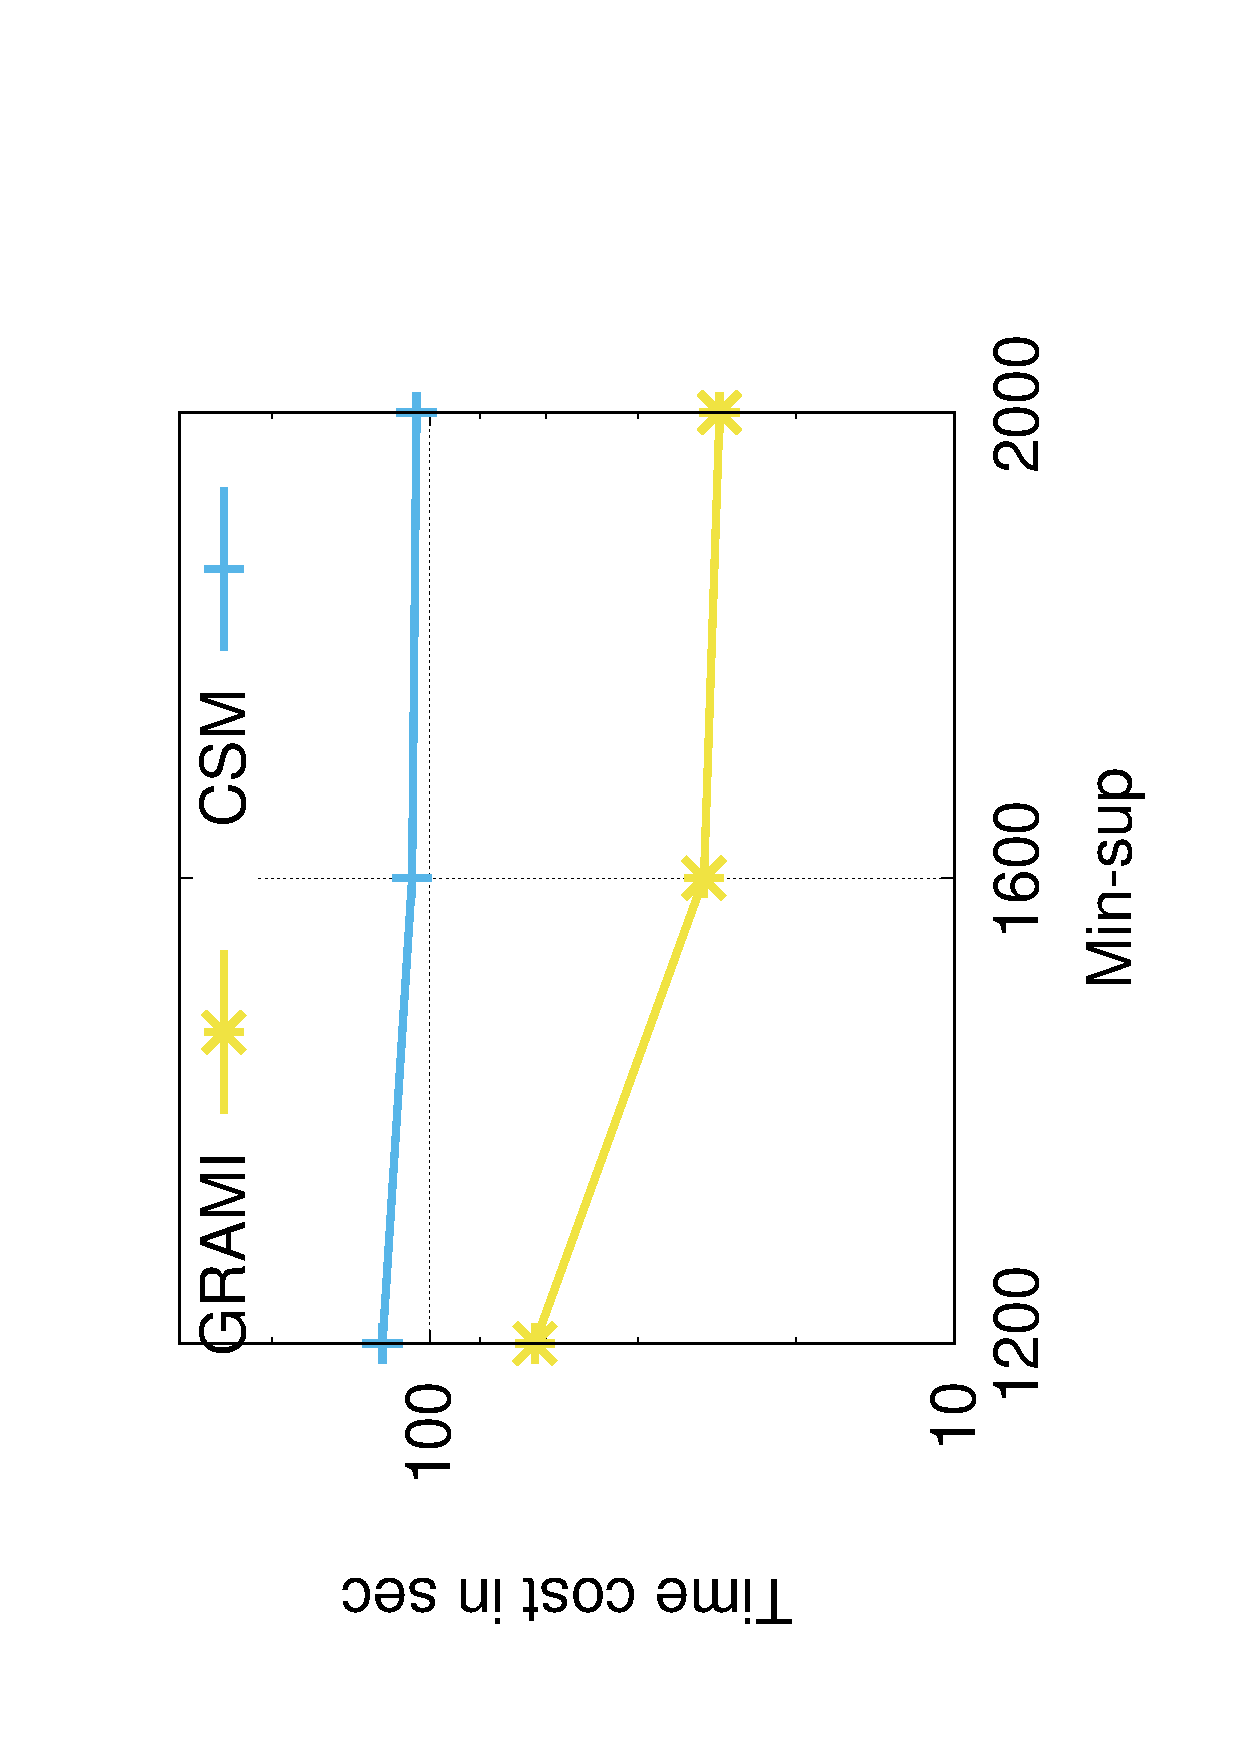
\includegraphics[scale=0.17, angle=270]{img2/fsm_lastfm}
% \label{fig:grami4}
% }
% \subfigure[{\scriptsize a subgraph with 8 auto-morphisms}]  {
% 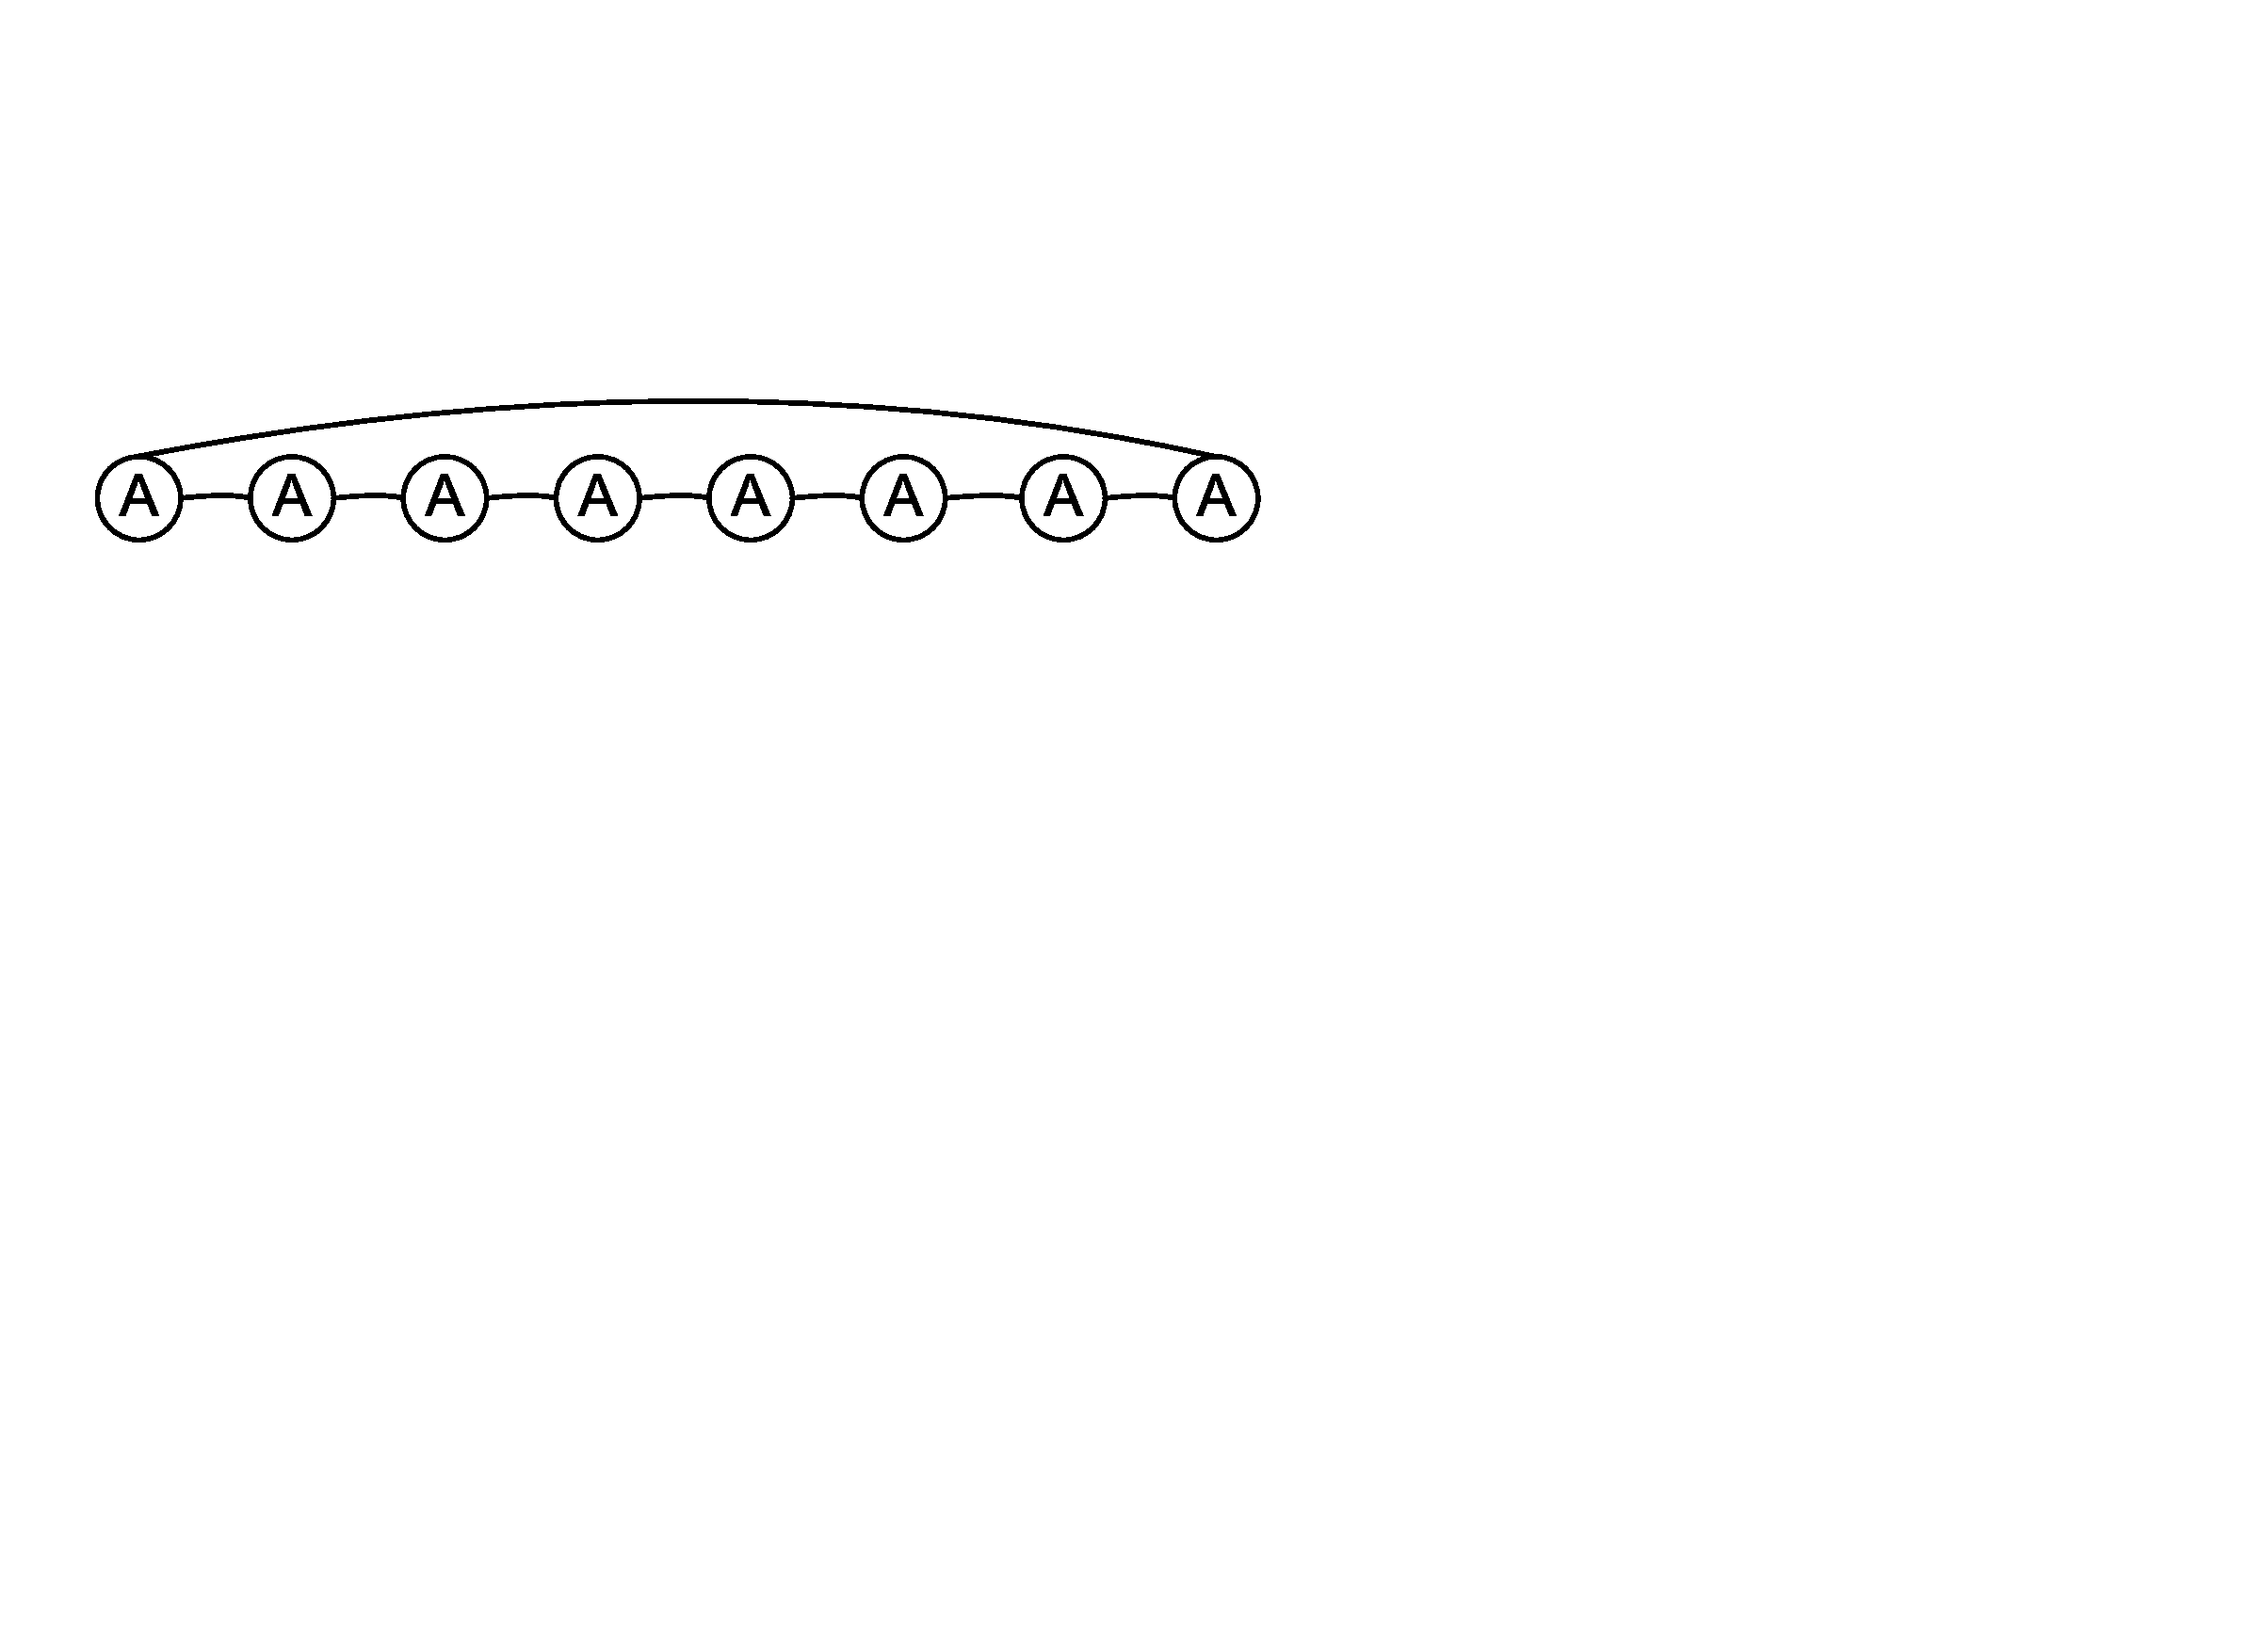
\includegraphics[scale=0.3]{img2/grami5}
% \label{fig:grami5}
% }

% \vspace{-2mm}
% \caption{\scriptsize Comparison with {\sf GRAMI}.}
% \label{fig:grami}
% \vspace{-6mm}
% \end{figure}


% \spara{$\bullet$ Comparison with {\sf GRAMI}.} Additionally, we provide the efficiency analysis of the problem, frequent subgraph mining (FSM), of our approach {\sf CSM}, compared with the state-of-art approach of FSM in a single large graph, {\sf GRAMI}\cite{EASK14}. As the state-of-art FSM algorithm in a single large graph, {\sf GRAMI} transforms the subgraph isomorphism to a CSP (constraint satisfaction problem) and makes optimization based on it. Corresponding to our experiment result, in most of the conditions, {\sf GRAMI} has a higher efficiency due to that it does not need to find all the occurrances. However, {\sf GRAMI} could not a good performance dealing with some subgraphs since the most significant optimization, push-down prunning, could hardly contribute in this case (All the positions are valid domains of the subgraph pattern and there are totally $8$ isomorphisms using MNI metric in Figure \ref{fig:grami5}). 


\section{Experimental Results}
\label{sec:experiments}

In this section, we provide the experimental result of our algorithm, noted as \textsc {CSM}. We also provide the instance-based method, noted as \textsc {GrowStore}, for comparison of frequent subgraph mining. In addition, we use \textsc {GraMi-VF3} as a comparison metric for subgraph isomorphism. GraMi is the state of the art method for frequent subgraph mining and VF3 is used for getting all instances of the frequent patterns. The algorithm is implemented in C++11 and compiled using gcc 7.4.0. All experiments are conducted on a Linux(Ubuntu 18) machine with 96 cores running at 2.1GHz with 251GB RAM and 8.5TB disk. Our experimental machine used a large memory size to accommodate the memory requirements of \textsc{GrowStore}.

% Unfortunately, the number of the instances could be exponential in worst cases, which means this number could still be very large in a not sparse data graph $G$. Except the MNI support calculation, we should also assign every instance to a group which it belongs to, which is extremely expensive. However, {\sf CSM} stores the subgraphs using the strategy of replica and avoid this huge drawback. As we demonstrate in the experimental result, {\sf CSM} has a much better performance than {\sf Grow and Store and GraMi plus VF3} in large and dense graphs. 


% Besides, we also provide the results of various input parameters, {\sf Min-sup}, hop-constraint $h$, and $k$ of {\sf Top-$k$}. All our experiments execute at GHz with $256$GB RAM and the implementation is carried out in C++.

\subsection{Experimental Setup}

\spara{Datasets - } Our experiments are based on the following real graph datasets. Their main characteristics are listed in Table \ref{tab:datasets}.


\par{\textit{Chemical}}. This dataset contains the undirected graph of a chemical compound in MCF7 Dataset of X.F. Yan\cite{YH02} with 207 vertices, 215 edges, 4 distinct node labels. Each node represents a chemical atom.

\par{\textit{Citeseer}}. Each vertex is a publication and label is the area of research in which that paper is published. Two vertices have an edge if one of the two papers is cited by the other and the edge label is the similarity measure between the two papers with a smaller label denoting stronger similarity. It has 3312 vertices, 4591 edges, ?? distinct node labels and 100 distinct edge labels(0-100) in it's original form but we scaled down the edge labels to 5. 

\par{\textit{Yeast}}. This dataset contains the undirected graph of proteins using the function as label, with ~4K vertices, ~79K edges and 26 distinct node labels. 

\par{\textit{Mico}}. It models Microsoft co-authorship information. Each vertex is an author and label is the field of interest. Edges represent collaboration between two authors and the edge label is the number of coauthored papers. It has ~100K vertices, 1.08M edges and ?? distinct node labels.

\par{\textit{LastFM}}. Each vertex is a user in the FM social network and label is the most frequent singer or music band that this user listens to. Two users who interact with each other will have a edge for connection. It has ~1.1M vertices, ~5.2M edges and ~83K distinct node labels.

\par{\textit{DBLP coauthor}}. Each vertex is an author and label is the conference in which that author is most publishe\d. Two vertices have an edge if the two authors have co-authored in at least 1 paper. It has ~1.7M vertices, ~7.4M edges and ~11K distinct node labels.

\par{\textit{DBLP citation}}. Each vertex is a publication and label is the conference in which that paper is published. Two vertices have an edge if one of the two papers is cited by the other. It has ~3.2M vertices, ~5.1M edges and ~11K distinct node labels.










\begin{table}[tb!]
	\vspace{-2mm}
	\begin{center}
		\vspace{-1mm}
		\centering
		\caption{Datasets and characteristics\label{tab:datasets}}
		\vspace{-3mm}
		\begin{tabular} {cccc}
			\hline
			Datasets  & Nodes & Edges  & Domain\\			 
			\hline 
			{\em Chemical}   &   207    &  205   & Biological\\
			{\em Yeast}   &   4K    &  79K  & Biological\\
			{\em MiCo}   &   100K    &  1M   & Publications\\ 
			{\em LastFM}   &   1.1M   &  5.2M & Social Network\\
			{\em DBLP Coauthor}   &   1.7M    &  7.4M   & Publications\\ 
			{\em DBLP Citation}   &   3.2M   &  5.1M   & Publications\\
			{\em Citeseer}   &   3K   &  4.5K & Publications\\
			
			\hline
		\end{tabular}
	\end{center}
	\vspace{-4mm}
\end{table}


\spara{Parameters.} There are $3$ different input parameters in the problem of correlated subgraph mining. The minimum image based support {\sf Min-sup}, the $k$ value of our {\sf Top-$k$} results, and the hop-constraint value $h$. We show the results of our experiments by varying the values of these input parameters. Increasing the value of {\sf Min-sup} results in a decrease of frequent subgraphs, increasing the value of $k$ results in an increase of output number, increasing the value of $h$ results in more correlated subgraph pairs.

% \par In brief, if we ignore the value of $k$, by decreasing the value of {\sf Min-sup}, and by increasing the value of $h$, we get more correlated subgraphs.
% \par We evaluate the efficiency of the approach by setting various input parameters and analyze the time cost. The time cost is recorded from the initialization to the end of the search.


% \spara{$\bullet$ Memory Requirements.} The dataset {\em DBLP} with input parameters, {\sf Min-sup}= $5000$, $k=200$, $h=2$ has the largest memory cost among all our experiments except setting $h=3$ of our {\sf CSM} approach, which is $512$GB$\times 1.8\%=9.216$GB.
% \par Compared with this acceptable memory cost, the algorithm {\sf iCSM} has a memory cost of $512$GB$\times 8.2\%=41.984$GB, after $8$ hours running and mined only hundreds of frequent subgraphs during processing the dataset {\em DBLP}. Even if we are patient enough to wait for the result of {\sf iCSM}, it is definitely about to crash before it reach the ceasing condition. This fact demonstrates that the memory cost of instance based method could only be tolerated when the data graph is sparse. However, our replica based storage has a acceptable memory cost towards the data graph which is both large and dense. 


% \begin{figure}[t!]
% \vspace{-2mm}
% \centering
% \subfigure[{\scriptsize {\sf Top-$3$} correlation of {\em Chemical}}]{
% 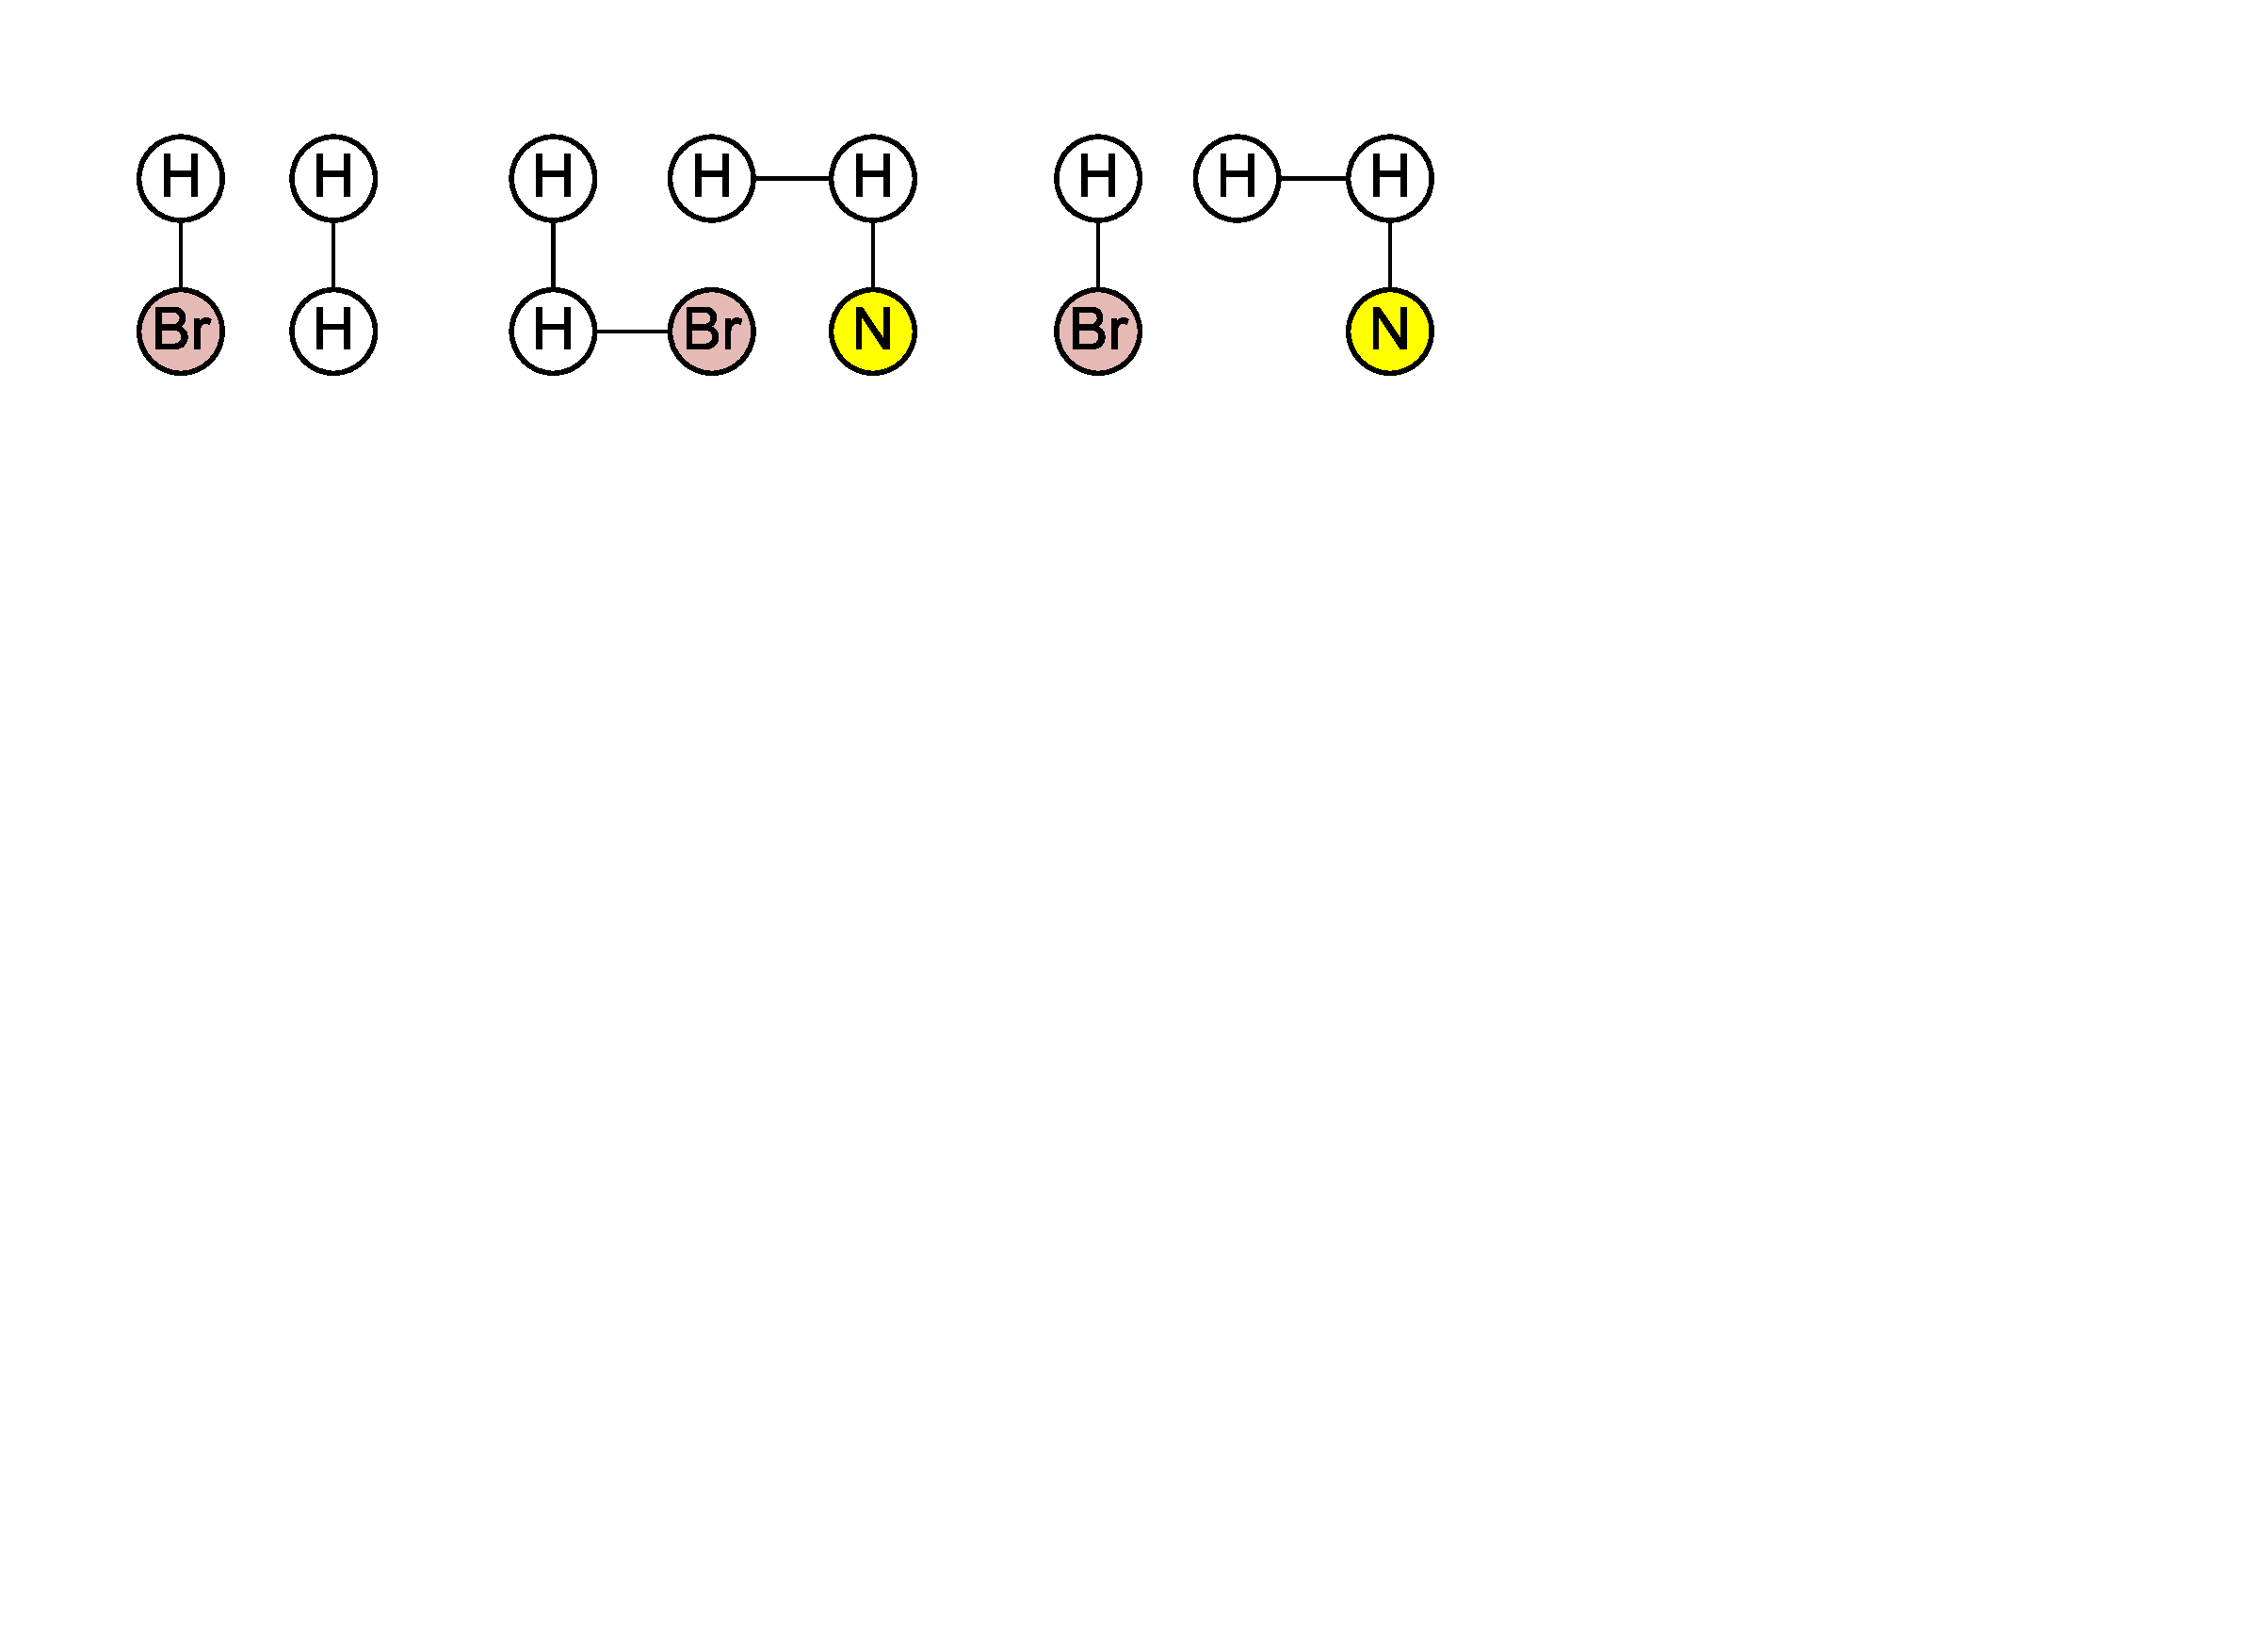
\includegraphics[scale=0.35]{images/tp_chemical}
% \label{fig:tp_chemical}
% }
% \subfigure[{\scriptsize {\sf Top-$3$} correlation of {\em Yeast}}]{
% 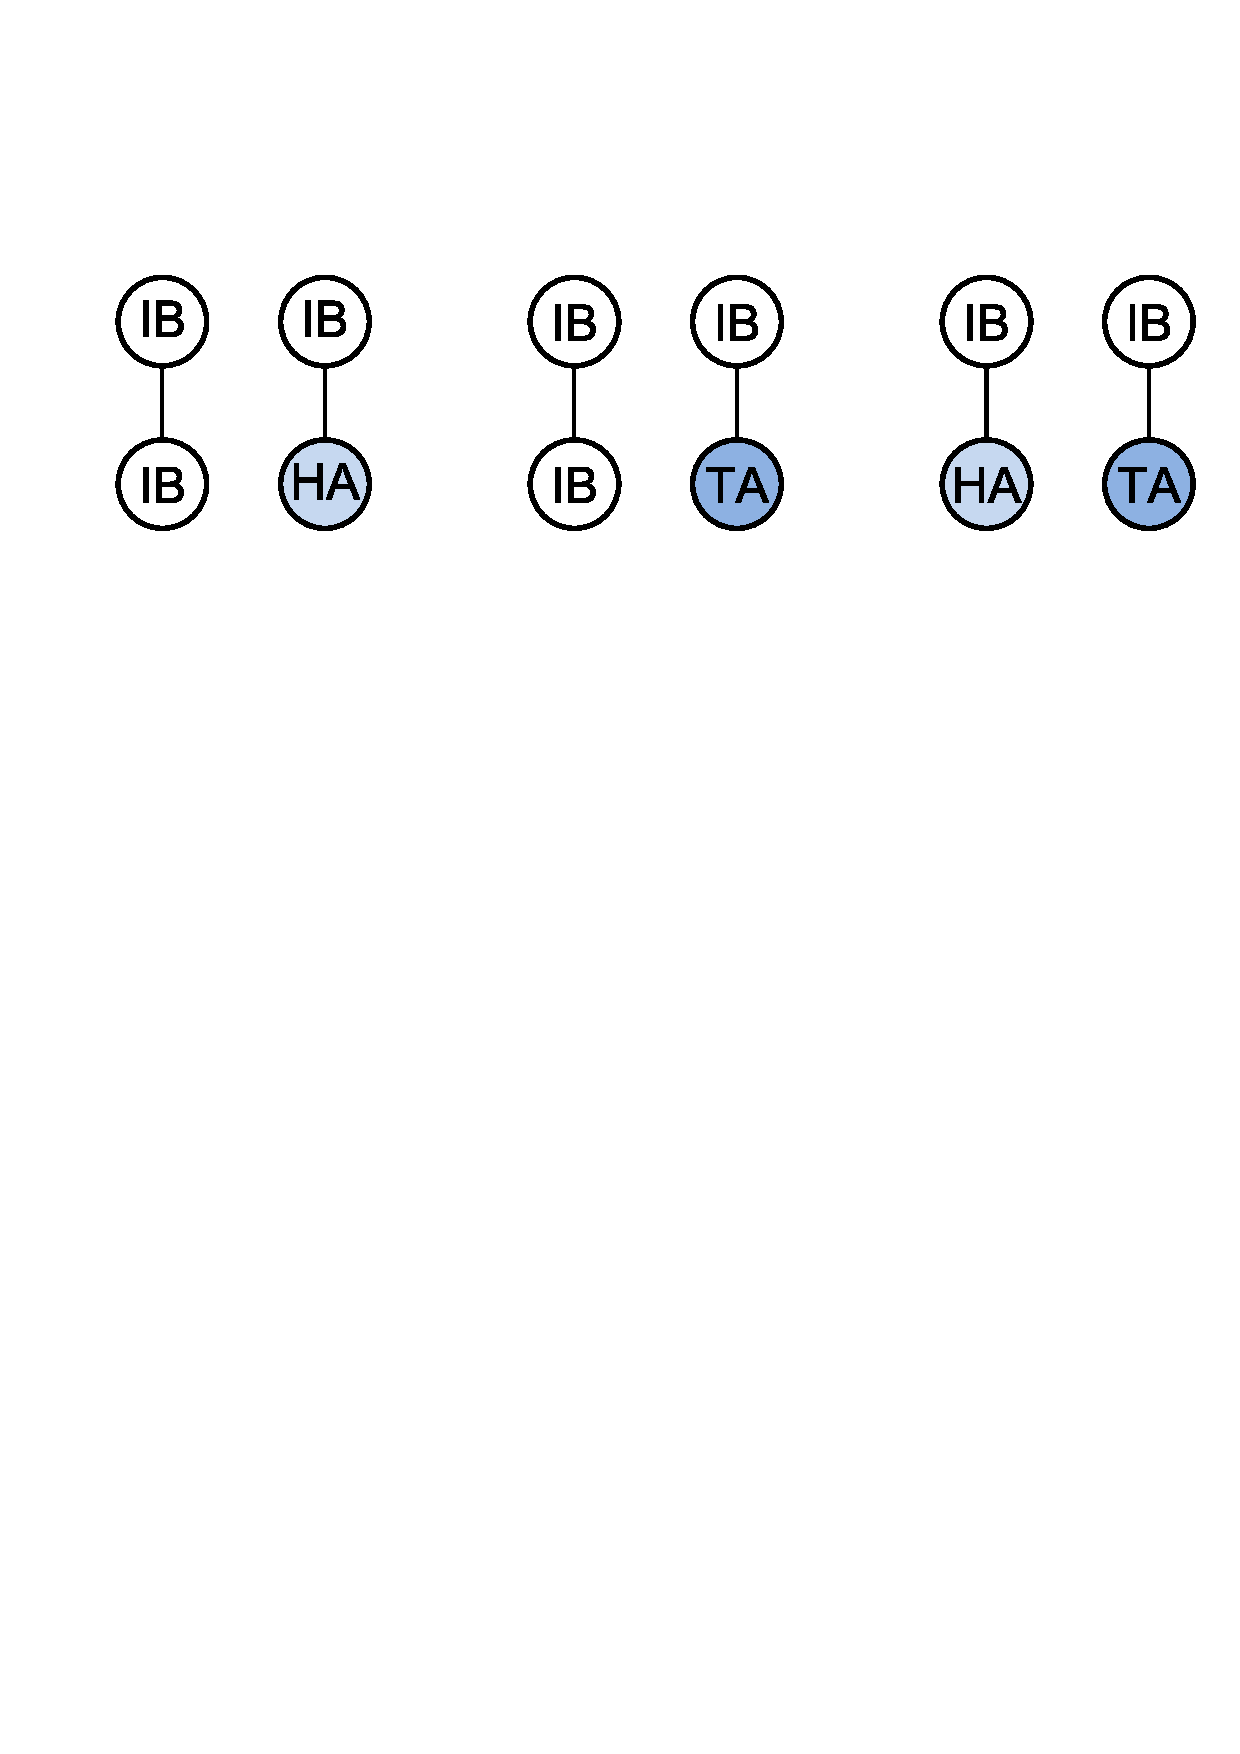
\includegraphics[scale=0.35]{images/tp_yeast}
% \label{fig:tp_yeast}
% }
% \subfigure[{\scriptsize {\sf Top-$3$} correlation of {\em DBLP}}]{
% 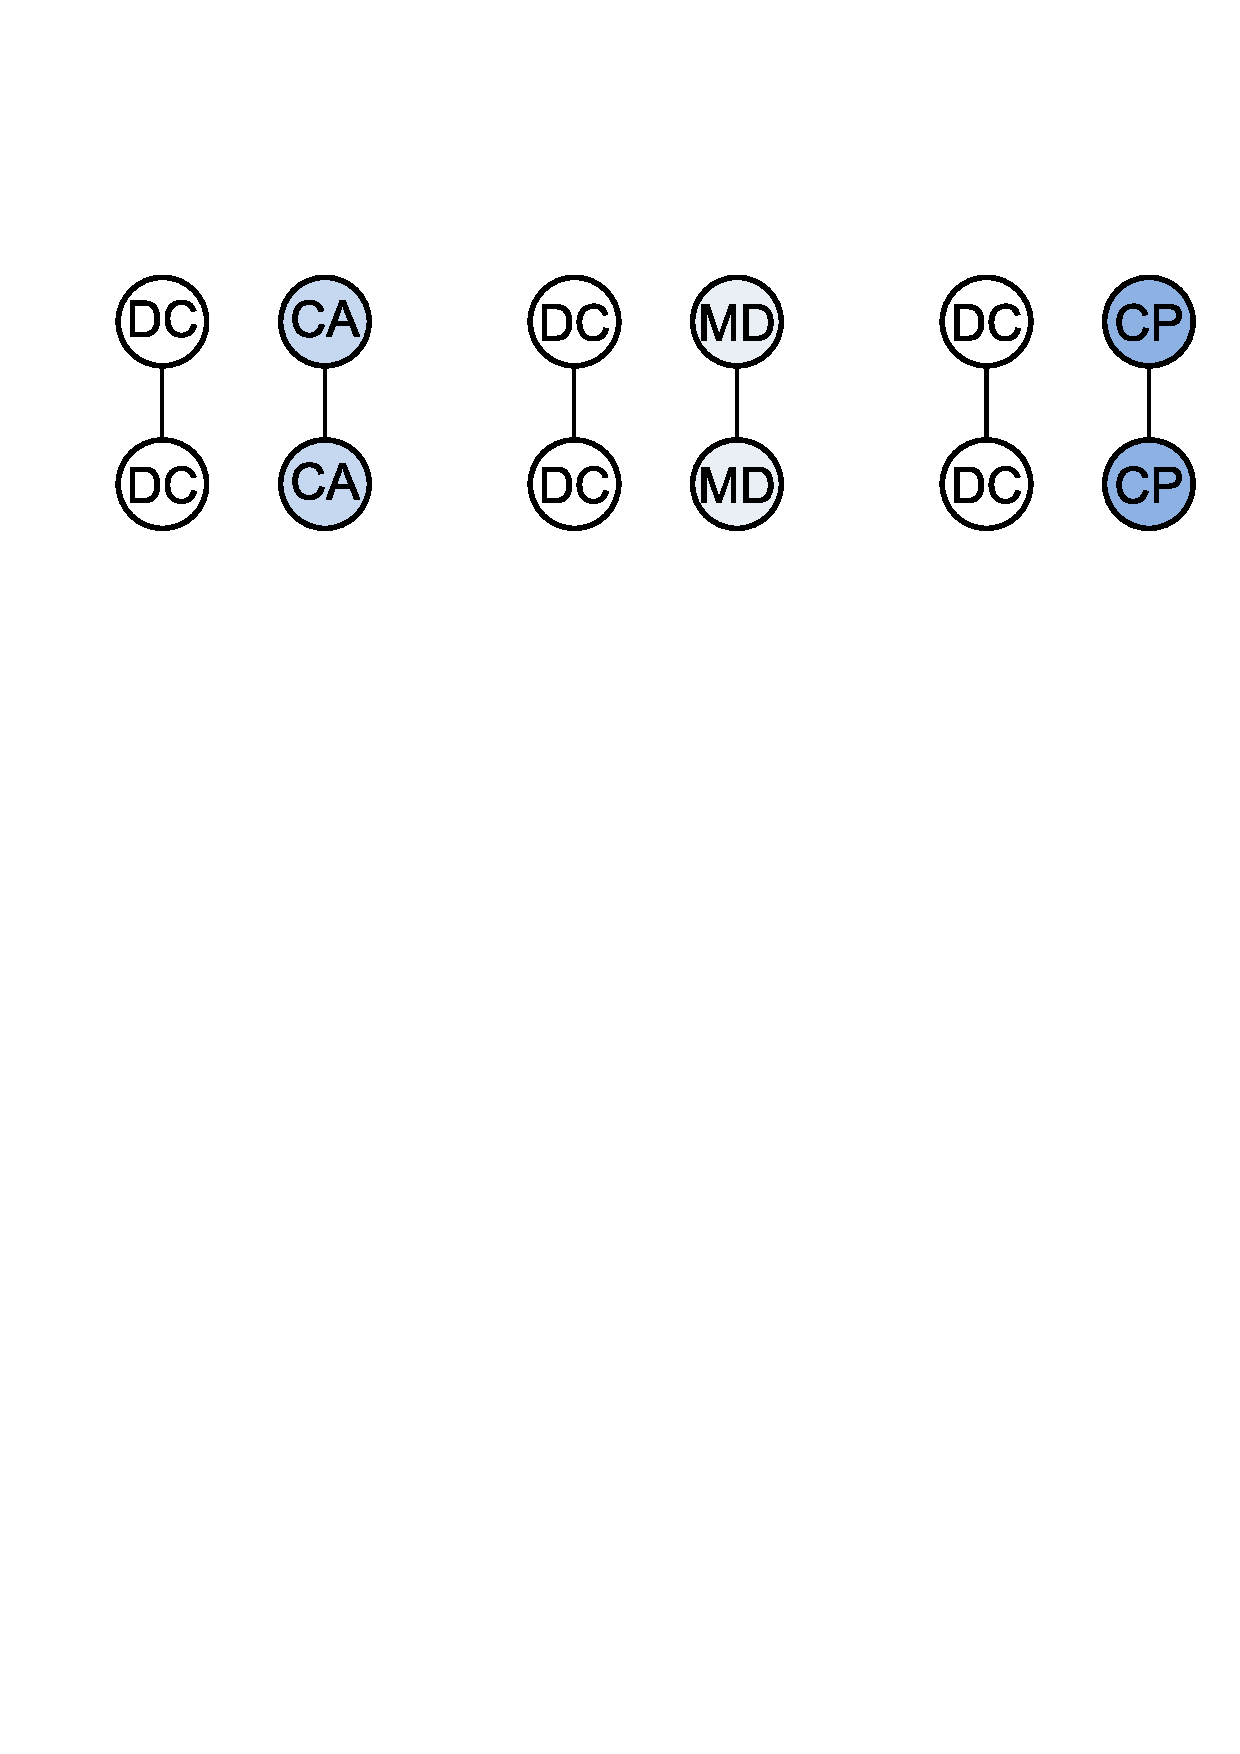
\includegraphics[scale=0.35]{images/tp_dblp}
% \label{fig:tp_dblp}
% }
% \subfigure[{\scriptsize {\sf Top-$3$} correlation of {\em LastFM}}]{
% 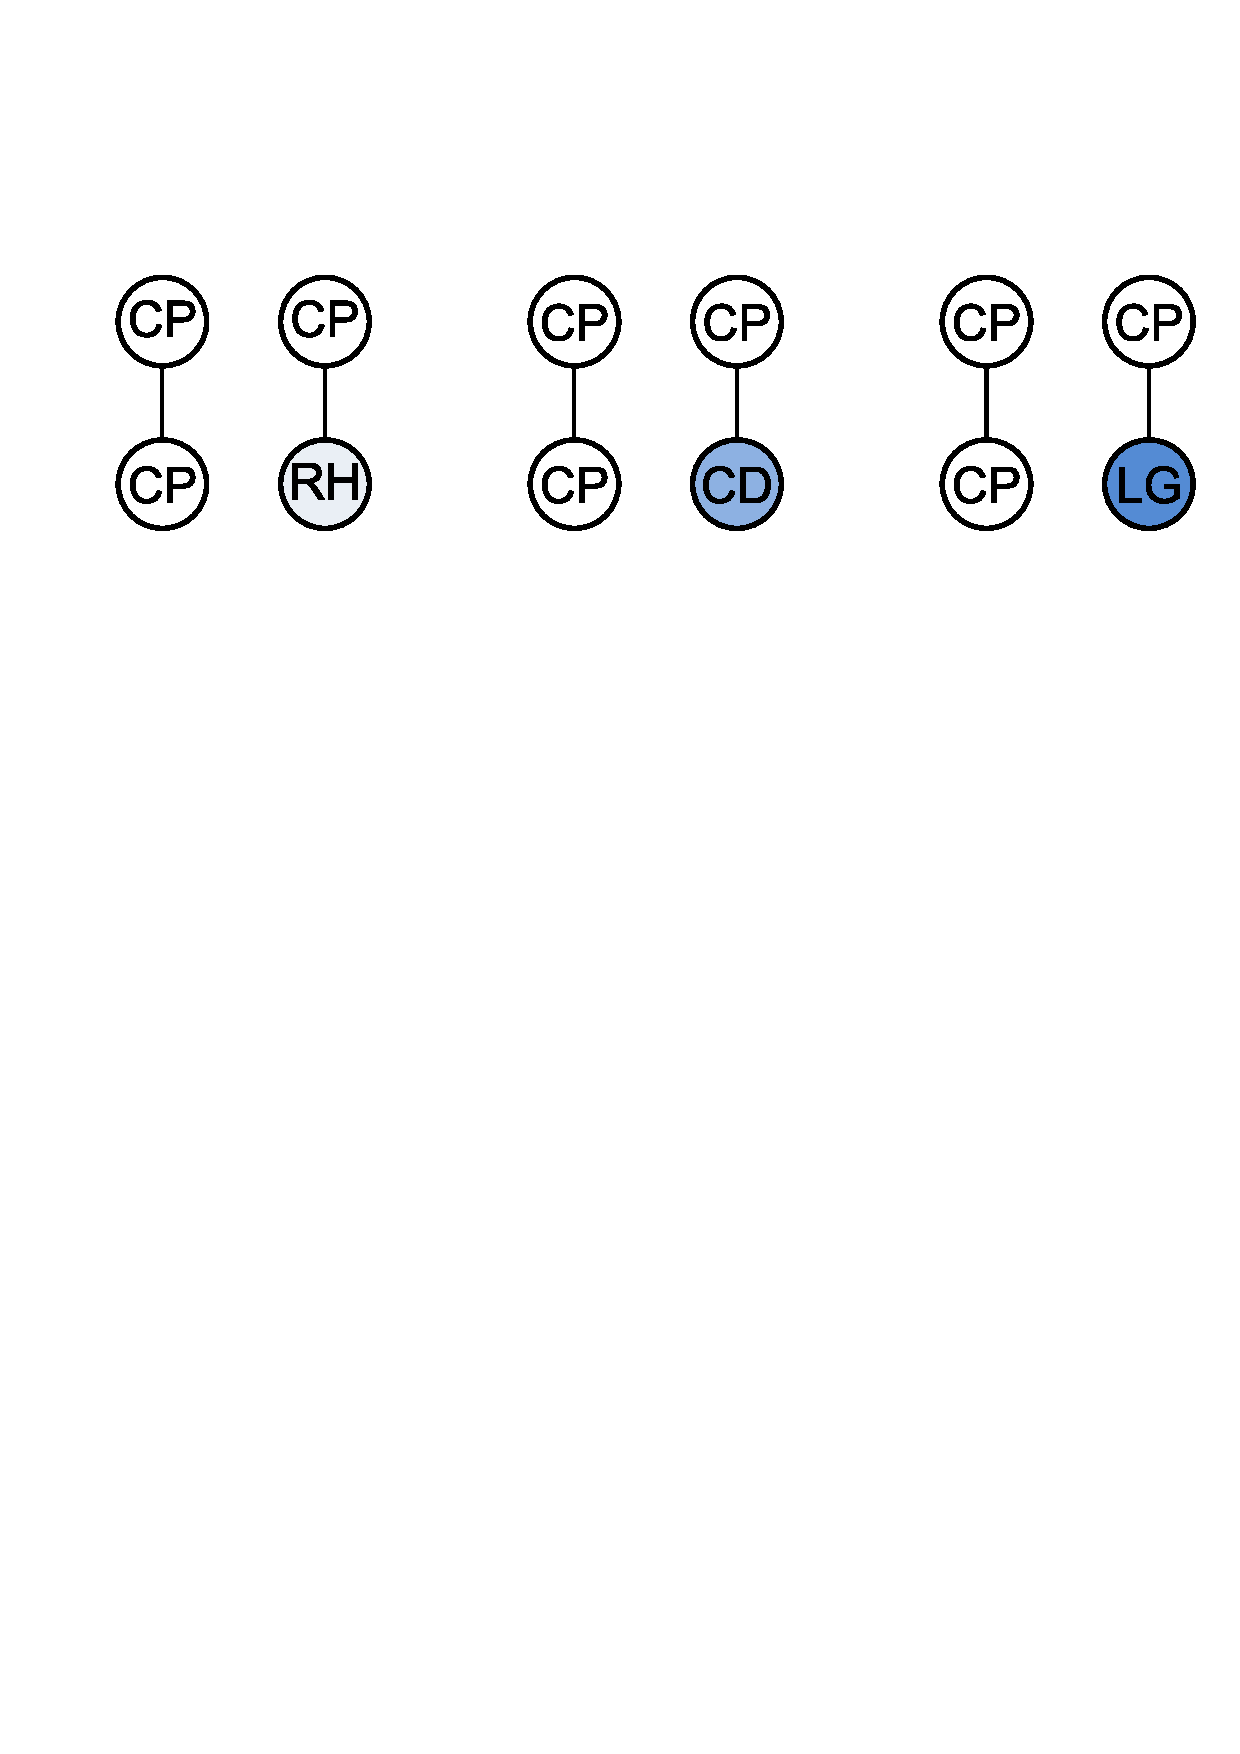
\includegraphics[scale=0.35]{images/tp_lastfm}
% \label{fig:tp_lastfm}
% }
% \subfigure[{\scriptsize {\sf Top-$3$} correlation of {\em LastFM}}]{
% 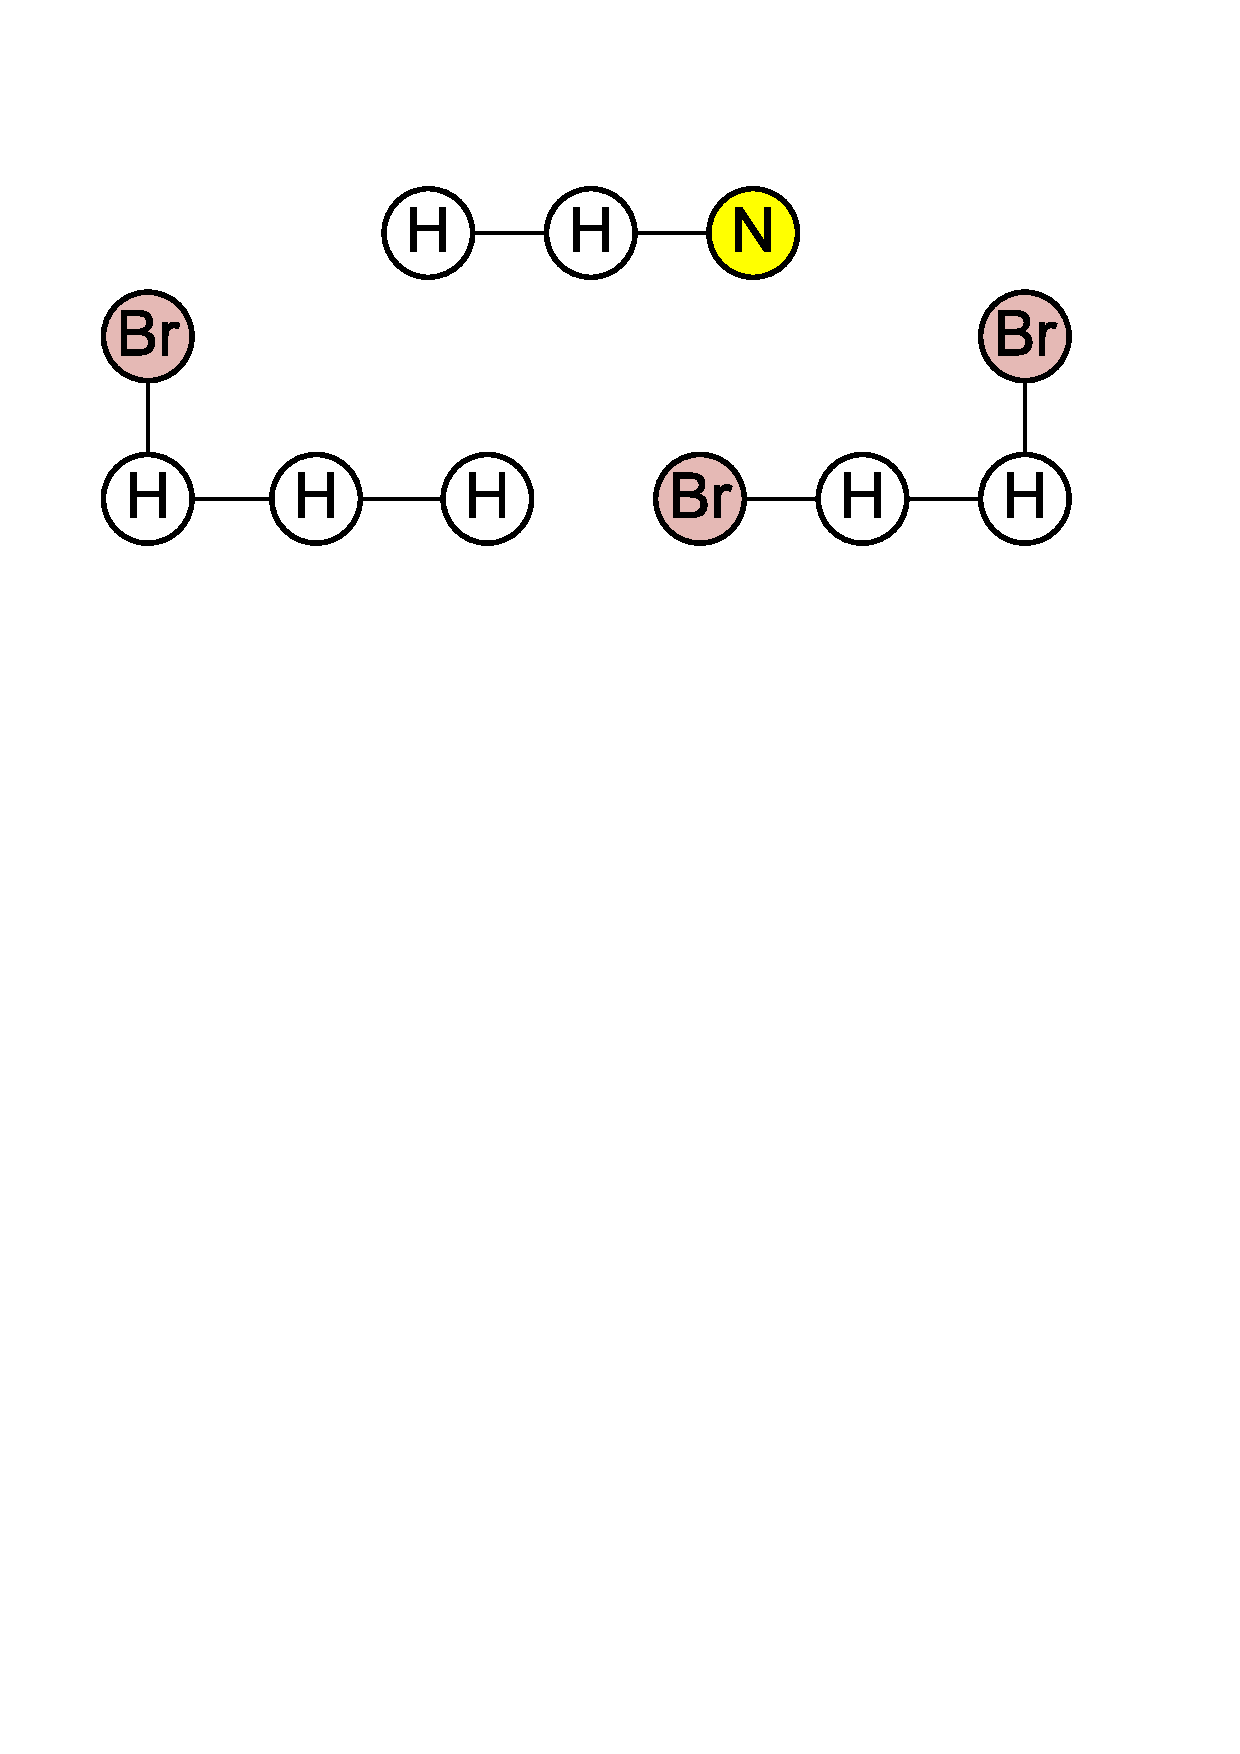
\includegraphics[scale=0.35]{images/tp_group}
% \label{fig:tp_group}
% }
% \vspace{-2mm}
% \caption{\scriptsize {\sf Top-$3$ correlations of datasets {\em (1)(2)(3)(4)}}.}
% \label{fig:tp}
% \vspace{-2mm}
% \end{figure}




\spara{Baselines} We compare our approximate algorithm with three baselines. The first one is the exact algorithm - \textsc{CSM-Exact} (Section \ref{sec:exact_algo}) . The second one is \textsc{GrowStore} which is an instance based approach for frequent subgraph mining. The third one is \textsc{GraMi-VF3} in which we use \textsc{GraMi}(??) for frequent subgraph mining and \textsc{VF3}(??) for subgraph isomorphism of all the frequent patterns which we get as an output from \textsc{GraMi} . We do not do correlation computation for $GraMi\ plus\ VF3$ as doing subgraph isomorphism for all the frequent patterns takes a significant amount of time which is larger than our entire approximate algorithm. \textsc{GrowStore} shows the advantage that we have in terms of memory for storing all the instances as discussed later. 
% For the datasets like {\em DBLP} which is very large but less dense, the number of the subgraphs dose not grow very quickly when the value of {\sf Min-sup} decrease. For the datasets like {\em Yeast} which is very dense, the number of the subgraphs increase at a multiple speed. However, the number of correlation is also much higher in dense graphs than that in sparse graphs because more degree also leads to the higher possibility of the correlations, which leads to an early termination and succeed to keep the efficiency of our approach.

\par \textit{Running Time Comparison.} The baselines are very slow for large and dense datasets so we compare the running times of our approximate algorithm with these baselines with an additonal constraint of size bound in patterns where we do not explore patterns which have more than 5 vertices. We do this because as the pattern size increases, the cost of computing the instances for that pattern grows exponentially. Figure \ref{fig:baseline_comp} shows comparison of running times with different baselines for different datasets when support is varied at $k=20$, $h=1$. 

\par{\textit{Memory Comparison and Usefulness of Replica.}} Replica provides an efficient way to store all the instances of a subgraph pattern whereas \textsc{GrowStore} stores all the instances. So in a frequent subgraph mining setting, \textsc{GrowStore} does work for small and less dense graphs but as the graph size increases or the graph becomes dense, the number of instances grow exponentially and thus the storage cost becomes too high. In figure \ref{fig:mem_comp}, we provide comparison of the memory requirements of our approach - \textsc{CSM} and \textsc{GrowStore} and it can be clearly seen that our approach helps in saving memory by a huge margin. In the plot of LASTFM, we have just one point for \textsc{GrowStore} because it gave memory error on a $256 GB$ machine for lower supports. The same happened for a smaller dataset like Citeseer as well for lower support. 

% Besides, we provide the total number of correlations with different input parameters {\sf Min-sup} and $h$, as Table \ref{tab:k-result}. The result is also easy to infer, which is, with lower {\sf Min-sup} or larger $h$, the total number of correlations would increase.

% \begin{table}[tb!]
% 	\vspace{4mm}
% 	\begin{center}
% 		\vspace{-1mm}
% 		\centering
% 		\caption{Correlated Subgraphs of various {\sf Min-sup} and $h$\label{tab:k-result}}
% 		\vspace{-3mm}
% 		\begin{tabular} {cccccc}
% 			\hline
% 			{Dataset} & {\sf Min-sup}  & $h=0$ & $h=1$ & $h=2$ & $h=3$ \\			 
% 			\hline 
% 			\multirow{3}{*}{Chemical} & 20 & 5 & 5 &  5 & 5 \\
% 			& 25   & 1 & 2 & 2 & 2 \\ 
% 			& 30   & 1 & 1 & 1 & 1 \\ 
% 			\hline 
% 			\multirow{3}{*}{Yeast} & 300 & 19 & 45 & 50 & 50 \\
% 			& 330   & 8 & 21 & 21 & 21 \\
% 			& 360   & 2 & 7 & 10 & 10 \\ 
% 			\hline 
% 			\multirow{3}{*}{DBLP} & 7000   &  2 & 31 & 146 & 311\\ 
% 			& 8000   &  0 & 16 & 94 & 196 \\
% 			& 9000   &  0 & 7 & 10 & 10 \\
% 			\hline 
% 			\multirow{3}{*}{LastFM} & 600   & 18 & 26 & 488 & 765 \\
% 			& 700   &  11 & 13 & 223 & 311 \\ 
% 			& 800   &  6 & 7 & 116 & 174 \\ 
% 			\hline
% 		\end{tabular}
% 	\end{center}
% 	\vspace{-8mm}
% \end{table}

% \begin{table}[tb!]
% 	\vspace{4mm}
% 	\begin{center}
% 		\vspace{-1mm}
% 		\centering
% 		\caption{Time cost comparison of {\sf CSM} and {\sf iCSM}\label{tab:icsm}}
% 		\vspace{-3mm}
% 		\begin{tabular} {ccccc}
% 			\hline
% 			Datasets & {\em Chemical} & {\em Yeast} & {\em DBLP} & {\em LastFM} \\			 
% 			\hline 
% 			{\sf CSM}   &  0.1 & 14 & 507 & 823 \\
% 			{\sf iCSM}   &  0.2 & over 10000 & over 10000 & over 10000 \\ 			
% 			\hline
% 		\end{tabular}
% 	\end{center}
% 	\vspace{-4mm}
% \end{table}
% \newline
% \newline
\begin{figure}[t!]
\vspace{-2mm}
\centering
\subfigure[{\scriptsize {\sf Hop-$1$, K-$20$} in {\em LASTFM}}]{
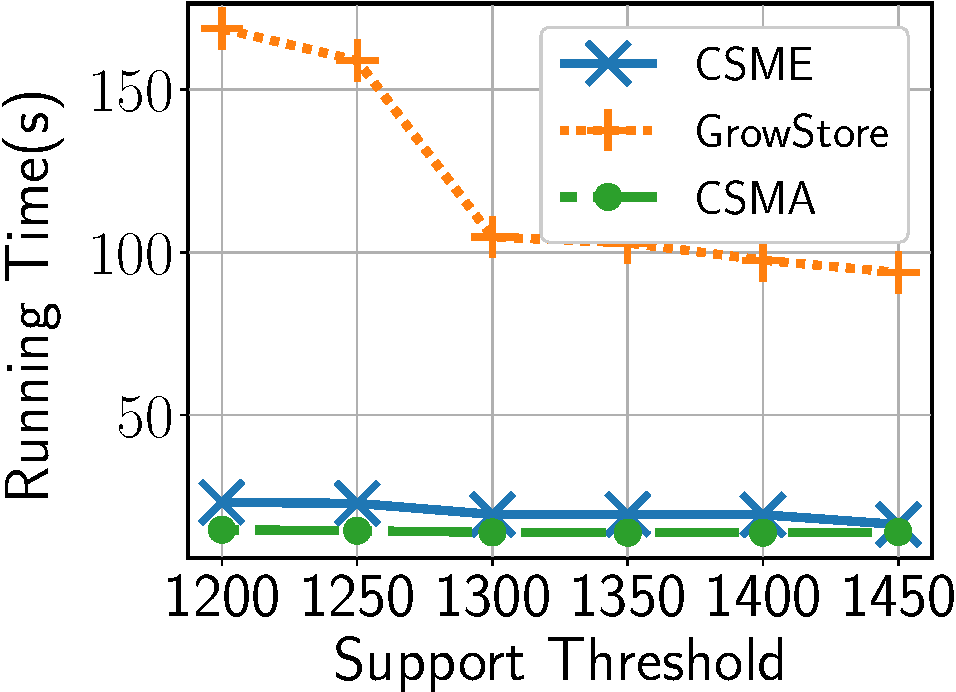
\includegraphics[scale=0.24]{img2/lastfm/lastfm_h1.pdf}
\label{fig:lastfm_h1}
}
\subfigure[{\scriptsize {\sf Hop-$1$, K-$20$} in {\em Mico}}]{
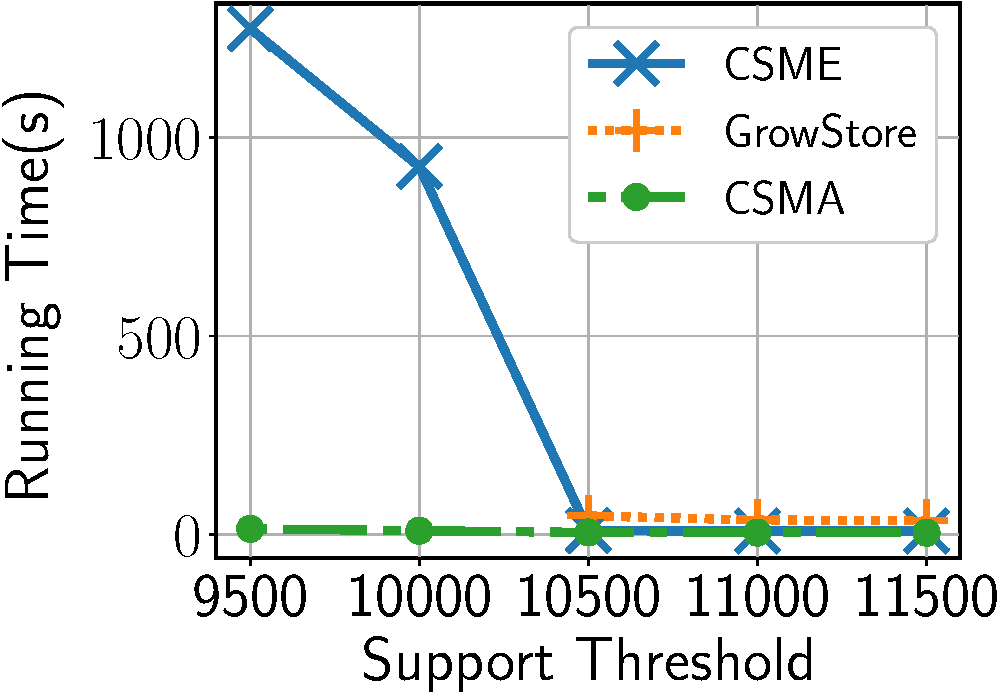
\includegraphics[scale=0.24]{img2/mico/mico_h1.pdf}
\label{fig:mico_h1}
}
\subfigure[{\scriptsize {\sf Hop-$1$, K-$20$} in {\em DBLP Coauthor}}]{
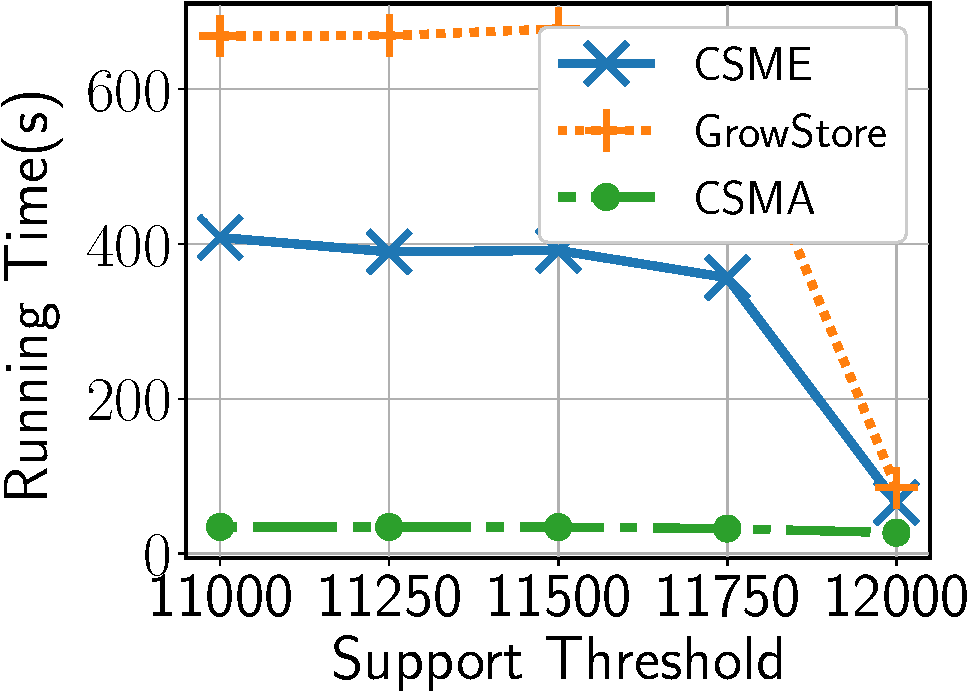
\includegraphics[scale=0.24]{img2/coauthordblp/coauthordblp_h1.pdf}
\label{fig:coauthordblp_h1}
}
% 
\subfigure[{\scriptsize {\sf Hop-$1$, K-$20$} in {\em DBLP Citation}}]{
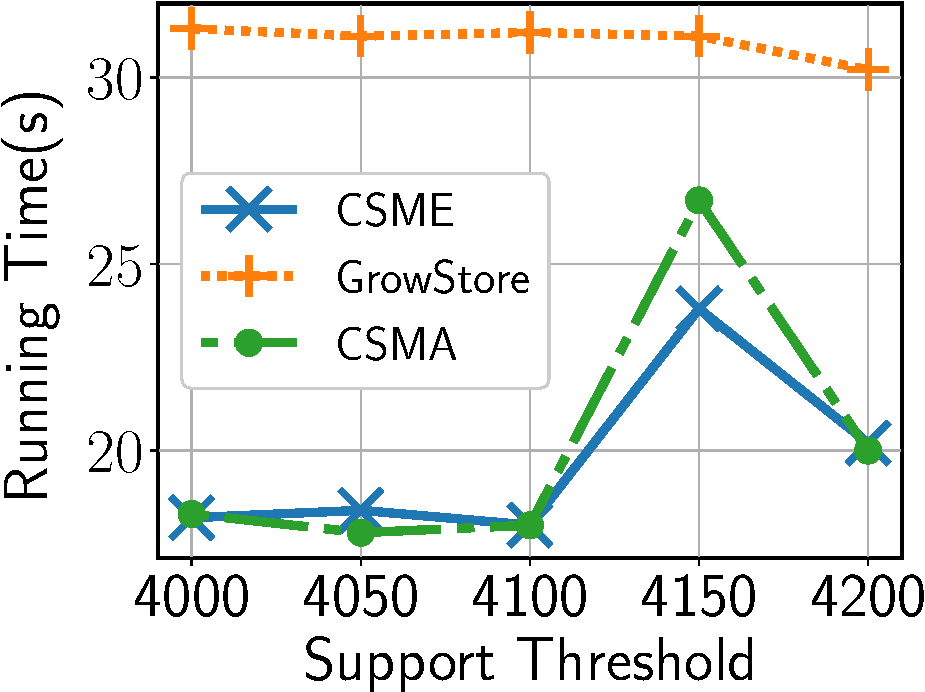
\includegraphics[scale=0.24]{img2/citationdblp/citationdblp_h1.pdf}
\label{fig:citationdblp_h1}
}
\vspace{-2mm}
\caption{\scriptsize {\sf Baseline Running Time Comparisons}.}
\label{fig:baseline_comp}
\vspace{-2mm}
\end{figure}

\begin{figure}[t!]
\vspace{4mm}
\centering
\subfigure[{\scriptsize {\sf Hop-$1$, K=$20$} in {\em LastFM}}] {
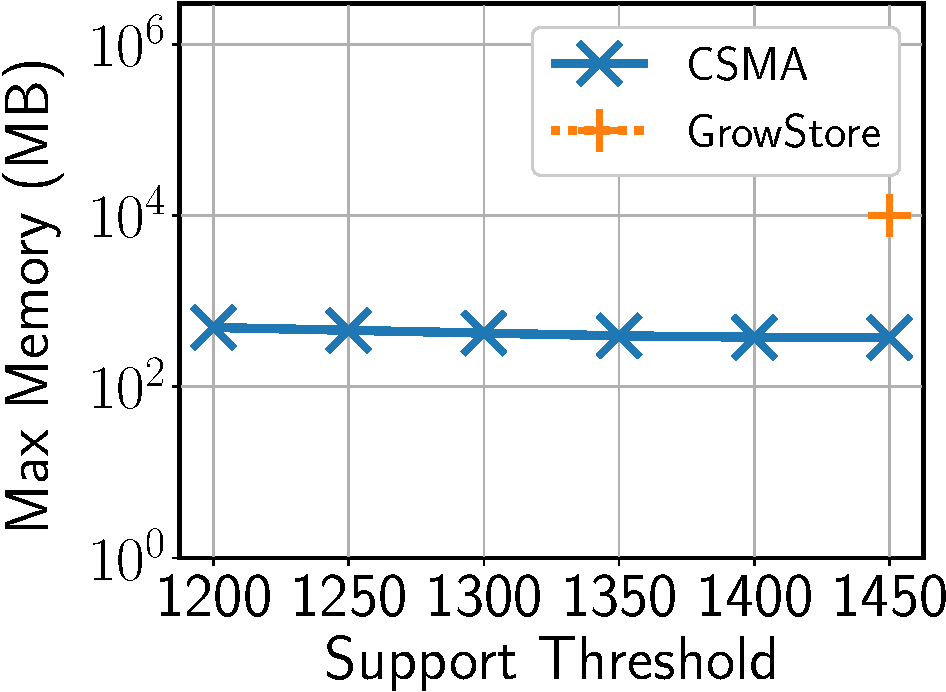
\includegraphics[keepaspectratio,scale=0.24]{img2/lastfm/lastfm_mem.pdf}
\label{fig:lastfm_mem}
}
\subfigure[{\scriptsize {\sf Hop-$1$, K-$20$} in {\em Citeseer}}]  {
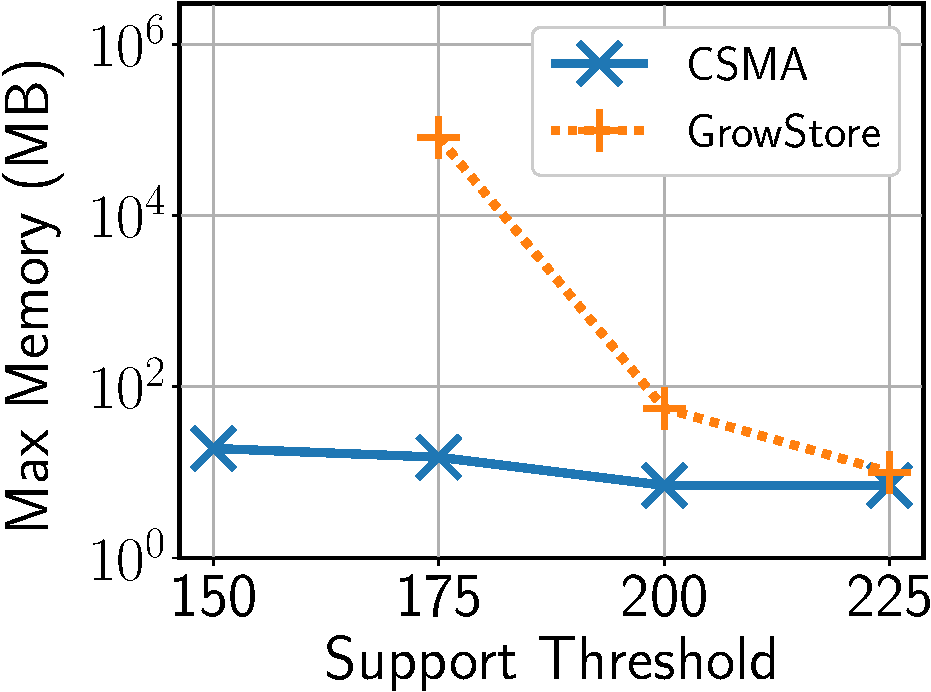
\includegraphics[keepaspectratio,scale=0.24]{img2/citeseer/citeseer_mem.pdf}
\label{fig:citeseer_mem}
}
\vspace{-2mm}
\caption{\scriptsize Baseline Memory Comparison.}
\label{fig:mem_comp}
\vspace{-2mm}
\end{figure}



% In Table \ref{tab:icsm}, we present the time cost (in sec) of all the datesets with setting {\sf Min-sup} $=20$ of {\em (1)}, {\sf Min-sup} $=200$ of {\em (2)}, {\sf Min-sup} $=5000$ of {\em (3)}, {\sf Min-sup} $=200$ of {\em (4)}, and all the datasets with $h=2$, $k=5$. The approach {\sf iCSM} could have a decent performance when the dataset is not dense, or relatively small, as the experiment on dataset {\em Chemical}. However, when the dataset becomes dense, it has to tackle with the exponential growth of the number of the instances, which is very expensive. In {\em Yeast} dataset, the most frequent single edge subgraph $Q$ has a MNI support $\sigma(Q)=1.4$K, but with the number of the instances $11$K. This number continues to grow at this speed and results in nearly $0.1$ million of the most frequent two edge subgraph. Suppose this number of the instances is $n$, after MNI support is calculated in $O(n)$ time, we have to spend another $O(n^2)$ time to finish the grouping process, which assigns each instance to a particular group. Eventually, this rapid growth of instance number leads to an unacceptable time cost of the approach {\sf iCSM}.


\subsection{Performance.}
We provide the experimental results of our approximate algorithm on large datasets from now on. 
\newline
\newline
\spara{Running Time Comparison.} Figure \ref{fig:approx_nobound} shows results of our approximation on four datasets at different $hops$ and varied $support$. The running time decreases with increasing support. As we increase hops, time and space required to compute proximate vertices index($CorV$) increases and as a result, the time taken for correlation computation also increases due to more correlations obtained. However, this can  sometimes lead to early termination as the top K set gets filled early. If the decrease in time due to this dominates the increase in time which is there, time may also decrease with increasing hops.
% From our empirical result, if there are enough $k$ correlations eligible, the time cost of all the datasets setting $h=0$ and $h=1$ could have no difference larger than $1$ sec. This is because through $h=1$ has a time increase from $h=0$, the total time cost at correlation calculation still does not dominate the total time cost. However, setting $h=2$ would receive a much higher time cost because the time cost of correlation calculation begins to dominate the total cost. However, when $h=3$, the time cost becomes extremely expensive and also has the memory cost over $256$GB. As a result, an approximation mining approach need to be proposed.


\begin{figure}[t!]
% \vspace{-2mm}
% \centering
\subfigure[{\scriptsize {\sf K-$20$} in {\em LastFM}}]{
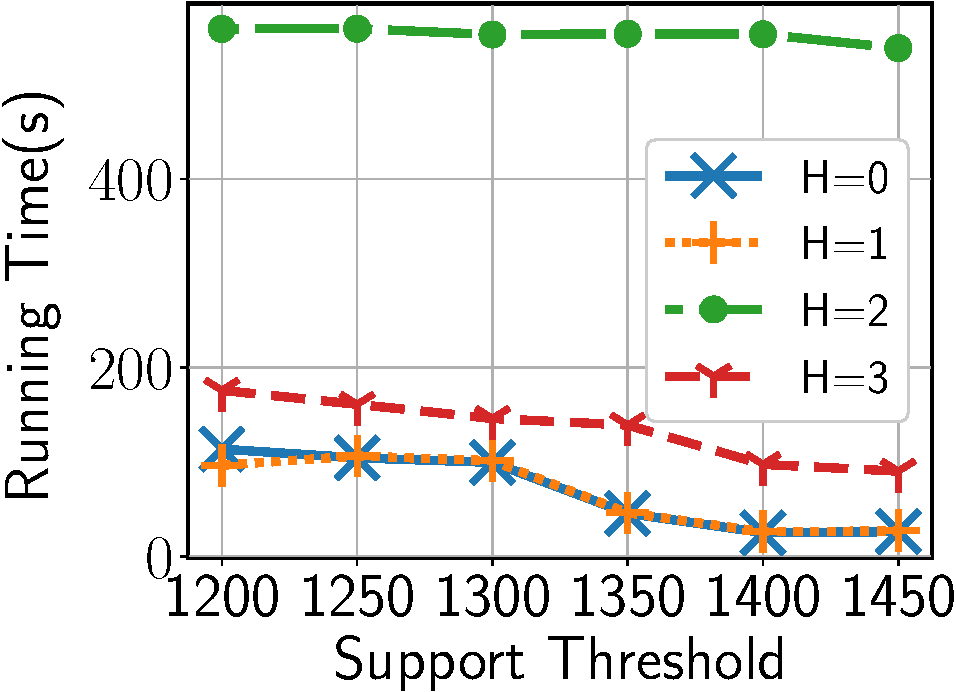
\includegraphics[keepaspectratio, scale=0.24, angle=0]{img2/lastfm/lastfm_running_time_nobound.pdf}
\label{fig:lastfm_nosb}
}
% width=\linewidth, height=\textheight, 
\subfigure[{\scriptsize {\sf K-$20$} in {\em Mico}}]{
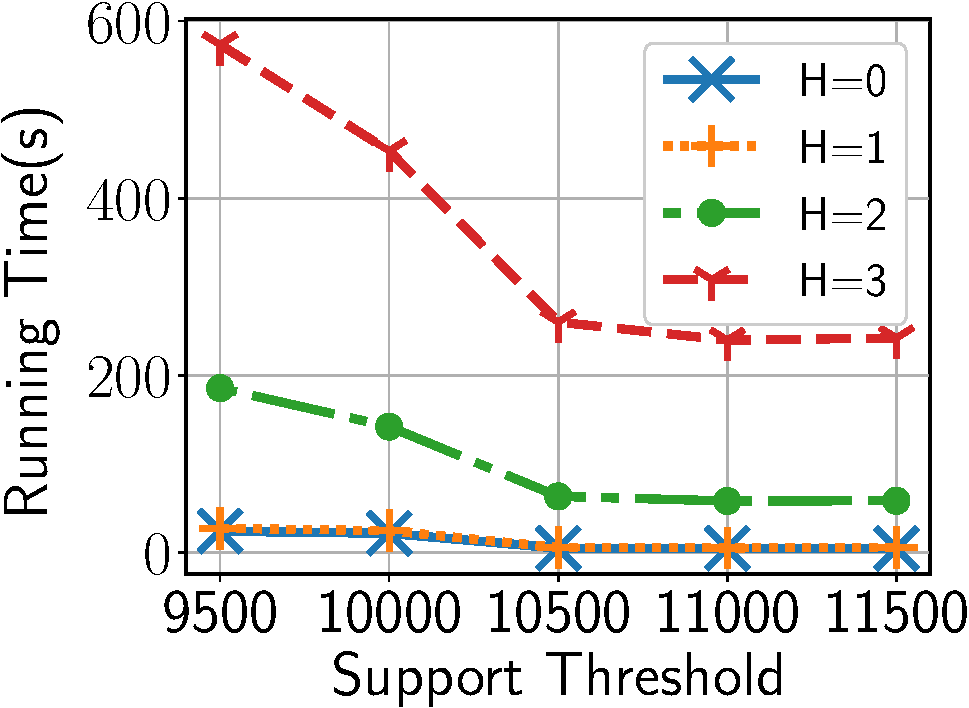
\includegraphics[keepaspectratio, scale=0.24, angle=0]{img2/mico/mico_running_time_nobound.pdf}
\label{fig:mico_nosb}
}
\subfigure[{\scriptsize {\sf K-$20$} in {\em DBLP Coauthor}}]{
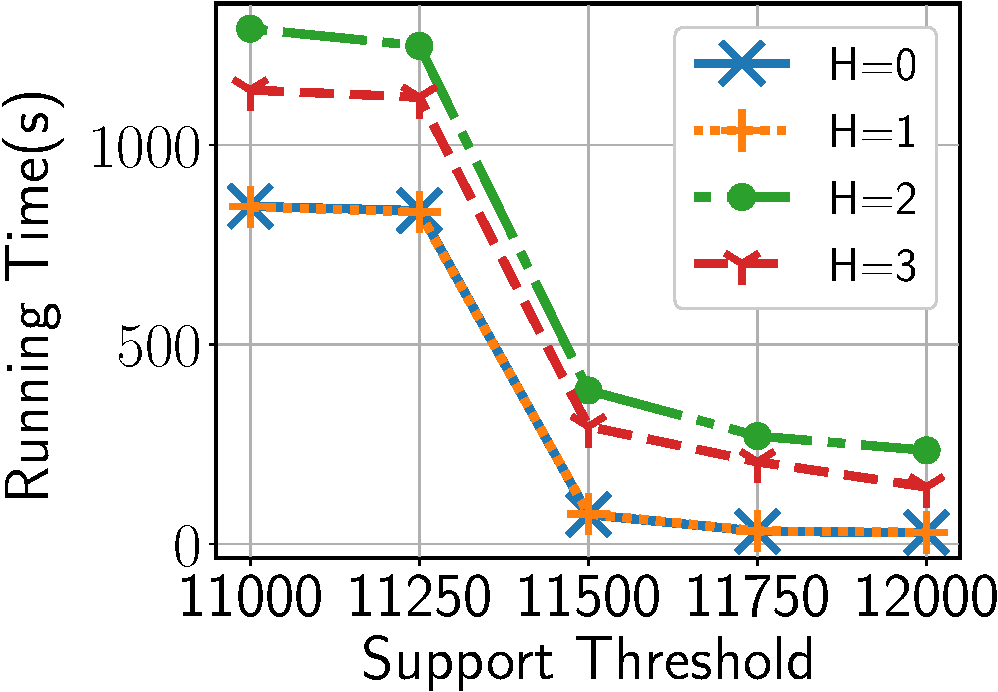
\includegraphics[keepaspectratio, scale=0.24, angle=0]{img2/coauthordblp/coauthordblp_running_time_nobound.pdf}
\label{fig:coauthordblp_nosb}
}
\subfigure[{\scriptsize {\sf K-$20$} in {\em DBLP Citation}}]{
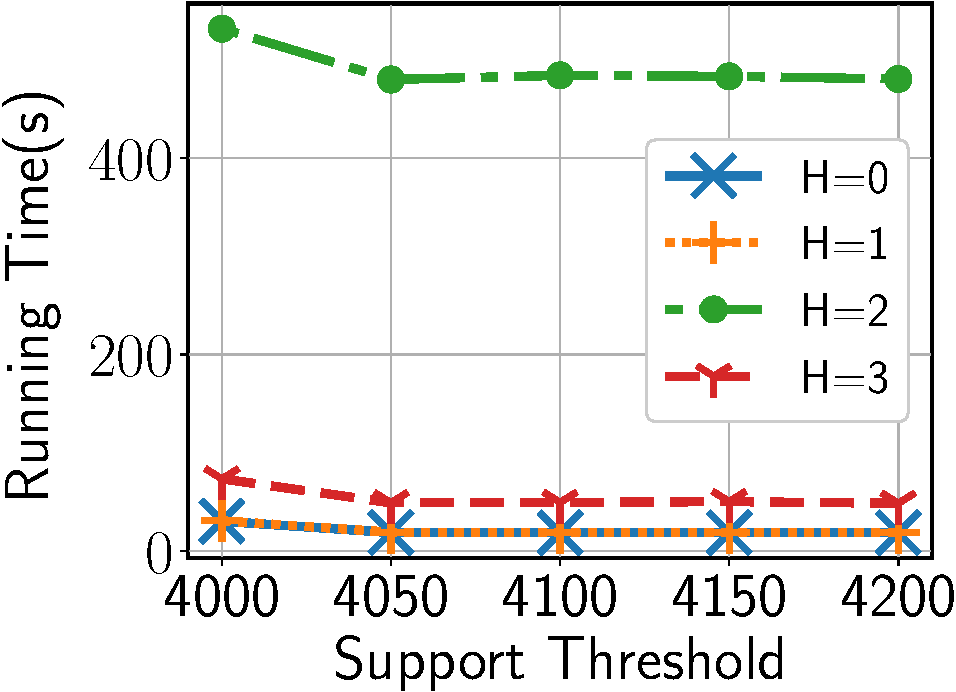
\includegraphics[scale=0.24, angle=0]{img2/citationdblp/citationdblp_running_time_nobound.pdf}
\label{fig:citation_nosb}
}
\vspace{-2mm}
\caption{\scriptsize CSMA Running Time Results.}
\label{fig:approx_nobound}
\vspace{-6mm}
\end{figure}


\begin{figure}[t!]
\vspace{4mm}
\centering
\subfigure[{\scriptsize {\sf Hop-$1$} in {\em LastFM}}] {
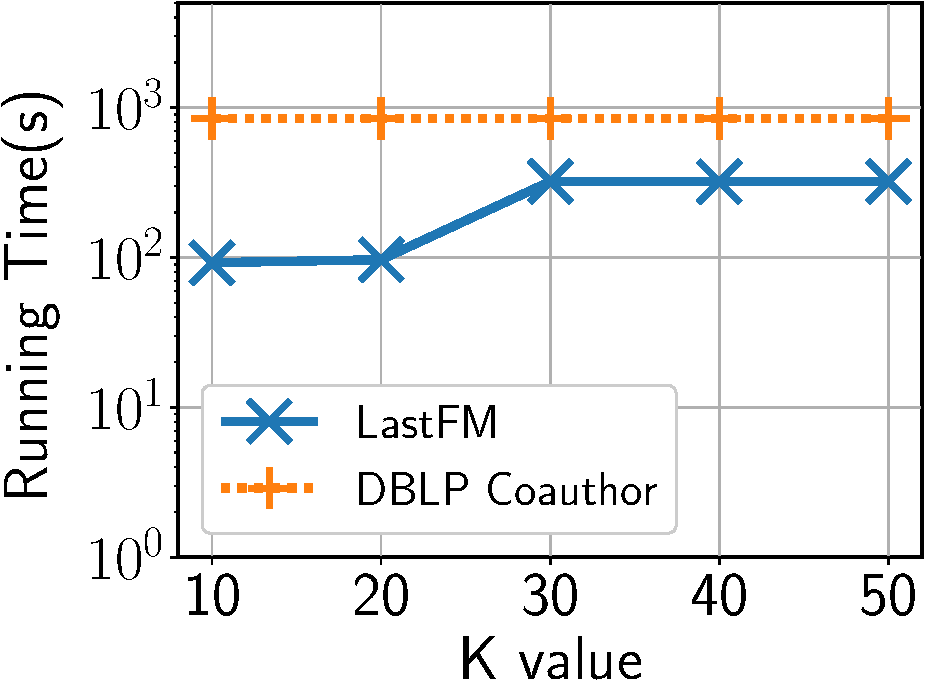
\includegraphics[keepaspectratio,scale=0.25]{img2/lastfm/lastfm_K_var_f.pdf}
\label{fig:lastfm_k}
}
% \subfigure[{\scriptsize {\sf Hop-$1$} in {\em Citeseer}}]  {
% 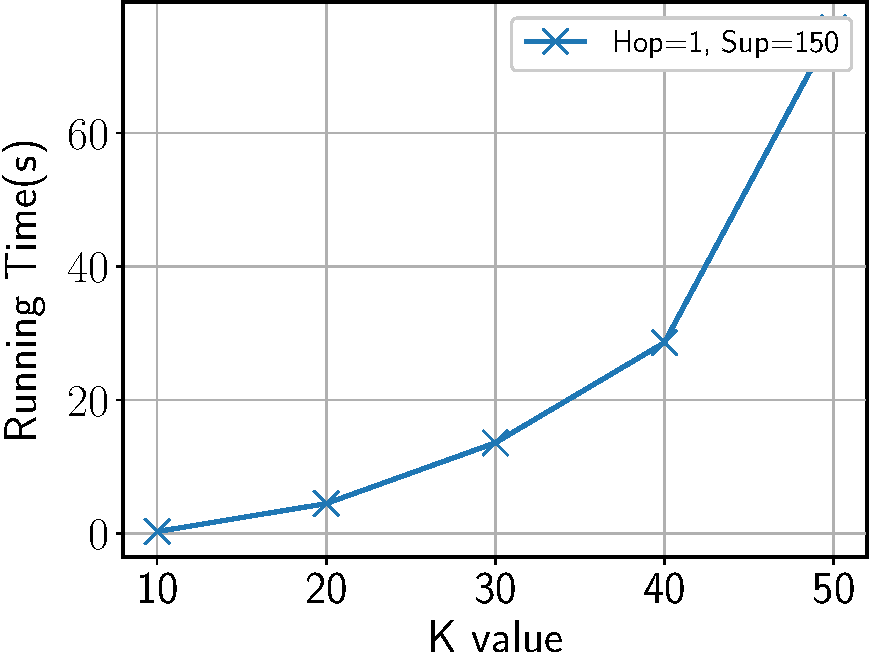
\includegraphics[keepaspectratio,scale=0.25]{img2/citeseer/citeseer_K_var.pdf}
% \label{fig:citeseer_k}
% }
\vspace{-2mm}
\caption{\scriptsize CSMA results with varying k, LASTFM $\sigma$=1200, DBLP Coauthor $\sigma$=11000.}
\label{fig:approx_k}
\vspace{-2mm}
\end{figure}

\par Figure \ref{fig:approx_k} shows results of our approximation algorithm with varying the $K$ parameter. As K increases, it is expected that more number of patterns will be processed and hence the running time should increase which can be seen in case of $LastFM$. However, it might happen that for a chosen support, the program is terminated after all the patterns are processed and there is no pattern remaining in the {\sf Search\ Queue} which means we cannot get more correlated patterns if we increase k. The time in such cases would stay the same after a certain K as can be seen in the case of $DBLP Coauthor$.

% \par Also, we provide the {\sf Top-$3$} correlations of datasets {\em (1)(2)(3)(4)} in Figure \ref{fig:tp} and give an example for the analysis of some results. As in Figure \ref{fig:tp_lastfm}, the result shows that {\em Coldplay} is a popular band and people who like {\em Coldplay} are very likely to have some friends who like {\em Coldplay} as well. Besides, people who like {\em Radiohead} are very likely to be in the social group where many people like {\em Coldplay}.

\eat{However, users may not be interested in some correlation like Figure \ref{fig:tp_dblp}. Due to its small size and symmetric structure, we can infer that if $h=1$, the subgraph pattern in Figure \ref{fig:result1} is very frequent. This job could already be done by frequent subgraph mining technique. Some users may also not interested in the correlation between just single edges. However, by simply limit the output correlation subgraph size, she can filter those small ones and reach her destination, like Figure \ref{fig:result2}.}



\spara{Comparison with other search strategies} We provide the comparison of our $Best$ $First$ $Search$ strategy with other search strategies, $Breadth$ $First$ $Search(BFS)$ and $Depth$ $First$ $Search(DFS)$. We count the number of patterns processed in all the three strategies by counting the number of patterns which are popped from the {\sf Search\ Queue}. Figure \ref{fig:dbfs} shows the results of these experiments on two datasets by varying $min-sup$ and $K$. 

\par In $DFS$, if we go to a branch where all patterns are frequent till a greater depth, it will lead to a lot of patterns being processed. $BFS$ processes all the patterns at a level as we can only stop processing patterns when all the patterns at a given depth have support less than the least correlation value in top k. However in best first search, there is no such restriction and we can stop as soon as we find a pattern with support less than the least correlation value in top k as all the other patterns will have a support less than or equal to the current pattern. In addition, the problem setting is such that patterns with higher frequency tend to have a higher correlation with other patterns and the best first strategy takes full advantage of this. However, if program gets terminated after all the patterns are processed and there are no patterns remaining in the {\sf Search\ Queue}, best first will have exactly same number of patterns explored as $BFS$ and $DFS$.


\begin{figure}[t!]
\vspace{4mm}
\centering
\subfigure[{\scriptsize {\sf K}=$20$, $Hop=1$ in {\em LastFM}}] {
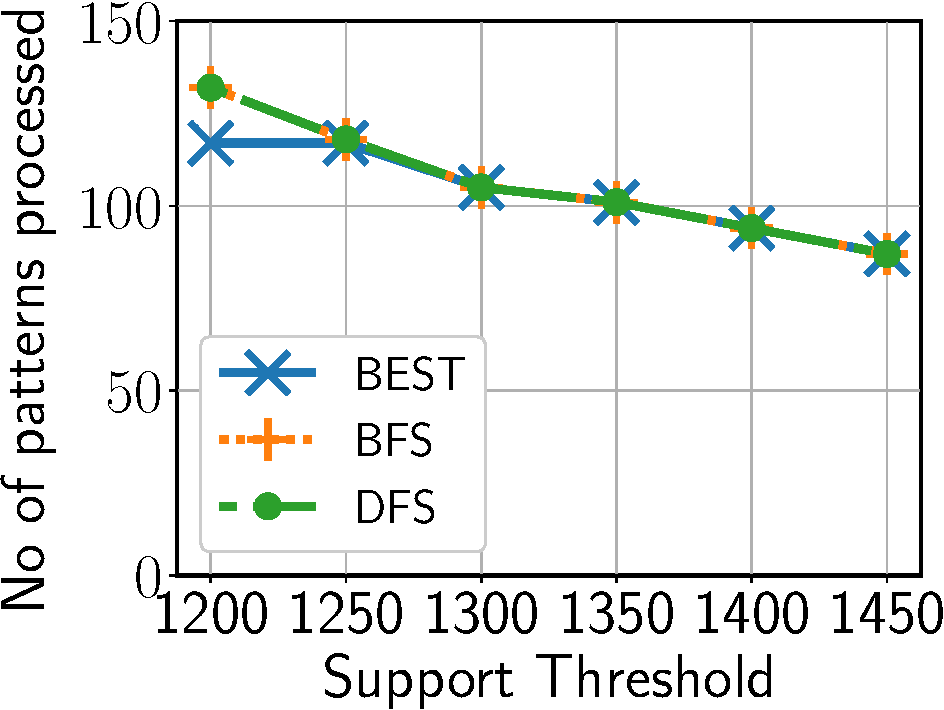
\includegraphics[keepaspectratio,scale=0.24, angle=0]{img2/lastfm/lastfm_bfsdfs_pop.pdf}
\label{fig:lastfm_bfsdfs_pop}
}
\subfigure[{\scriptsize {\sf Sup}=$1200$, $Hop=1$ in {\em LastFM}}] {
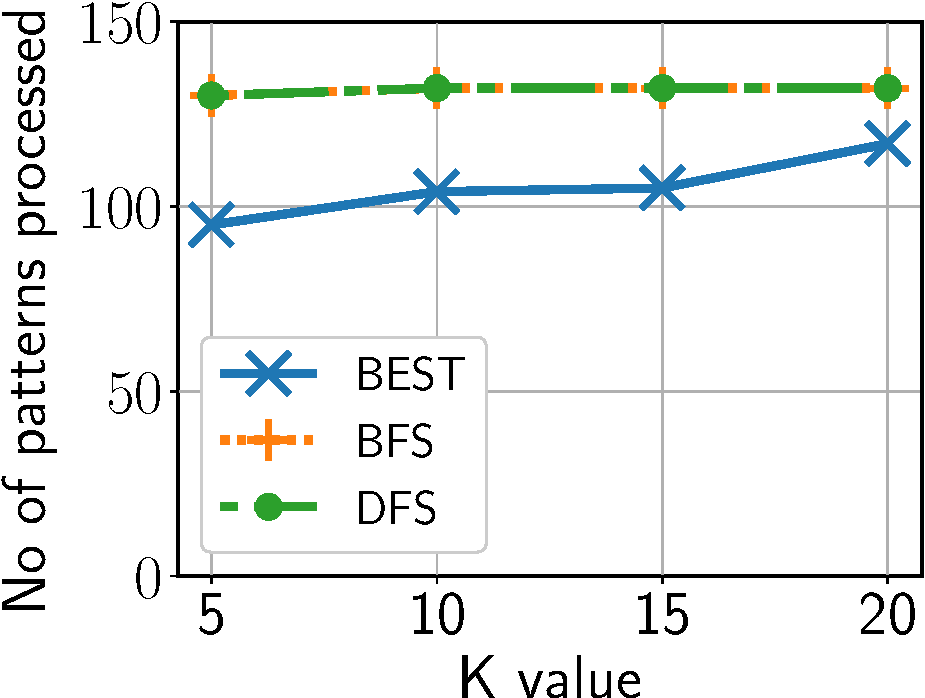
\includegraphics[keepaspectratio,scale=0.24, angle=0]{img2/lastfm/lastfm_bfsdfs_pop_k.pdf}
\label{fig:lastfm_bfsdfs_pop_k}
}
\subfigure[{\scriptsize {\sf K}=$20$, $Hop=1$ in {\em Chemical}}]  {
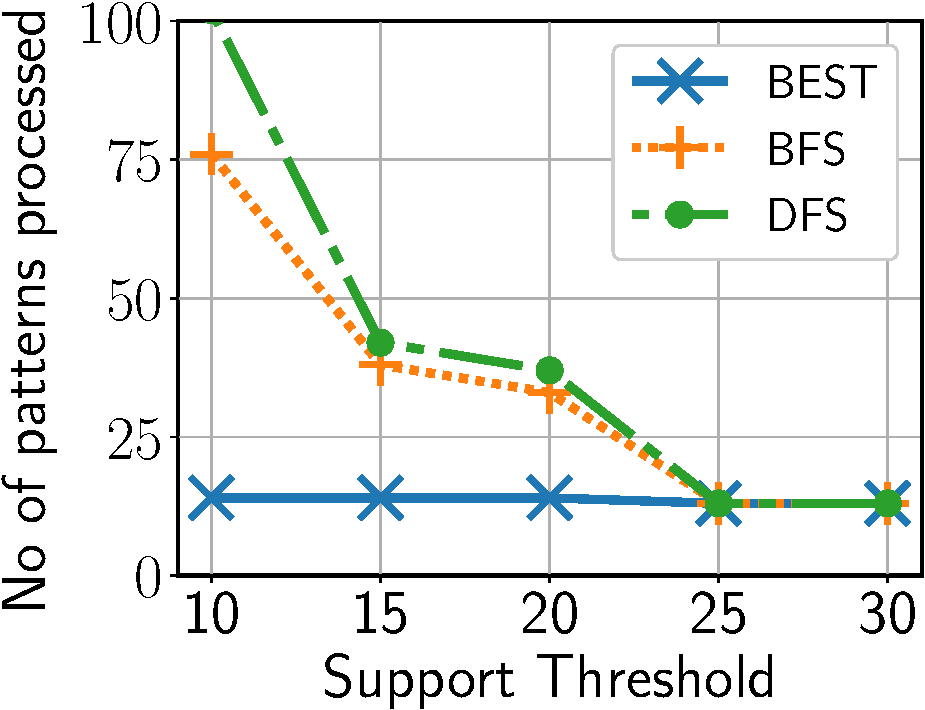
\includegraphics[keepaspectratio,scale=0.24, angle=0]{img2/chemical/chemical_bfsdfs_pop.pdf}
\label{fig:chemical_bfsdfs_pop}
}
\subfigure[{\scriptsize{\sf Sup}=$10$, $Hop=1$ in {\em Chemical}}]  {
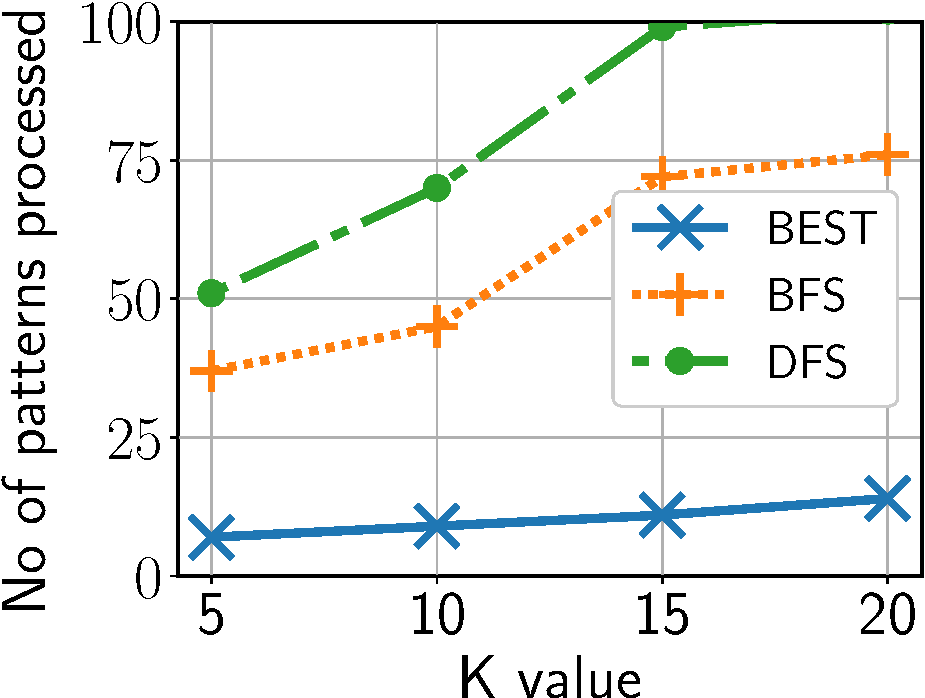
\includegraphics[keepaspectratio,scale=0.24, angle=0]{img2/chemical/chemical_bfsdfs_pop_k.pdf}
\label{fig:chemical_bfsdfs_pop_k}
}

\subfigure[{\scriptsize {\sf K}=$20$, $Hop=1$ in {\em DBLP Citation}}]  {
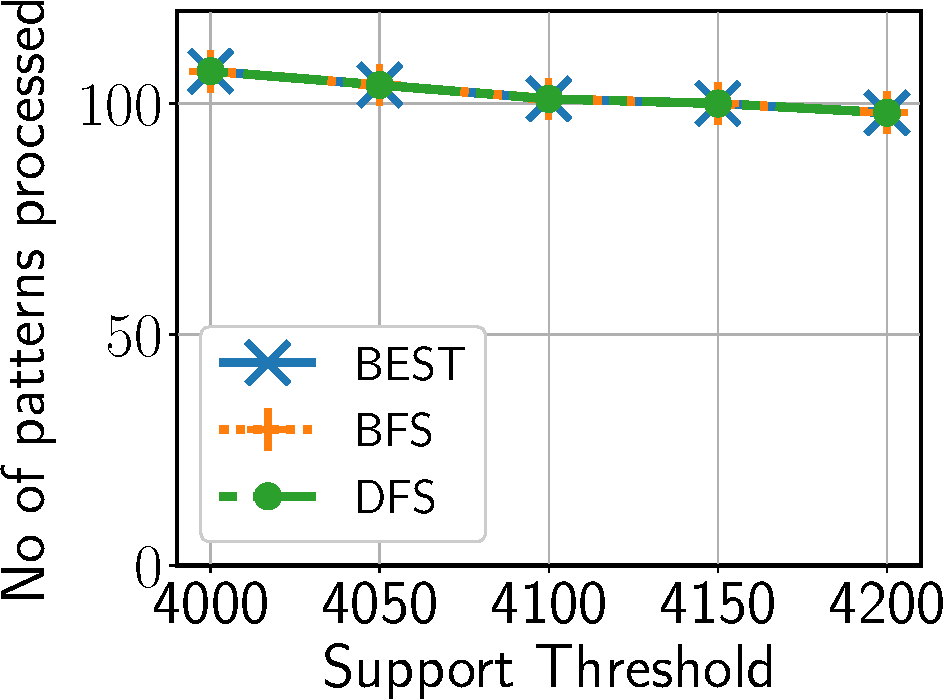
\includegraphics[keepaspectratio,scale=0.24, angle=0]{img2/citationdblp/citationdblp_bfsdfs_pop.pdf}
\label{fig:chemical_bfsdfs_pop}
}
\subfigure[{\scriptsize{\sf Sup}=$10$, $Hop=1$ in {\em DBLP Citation}}]  {
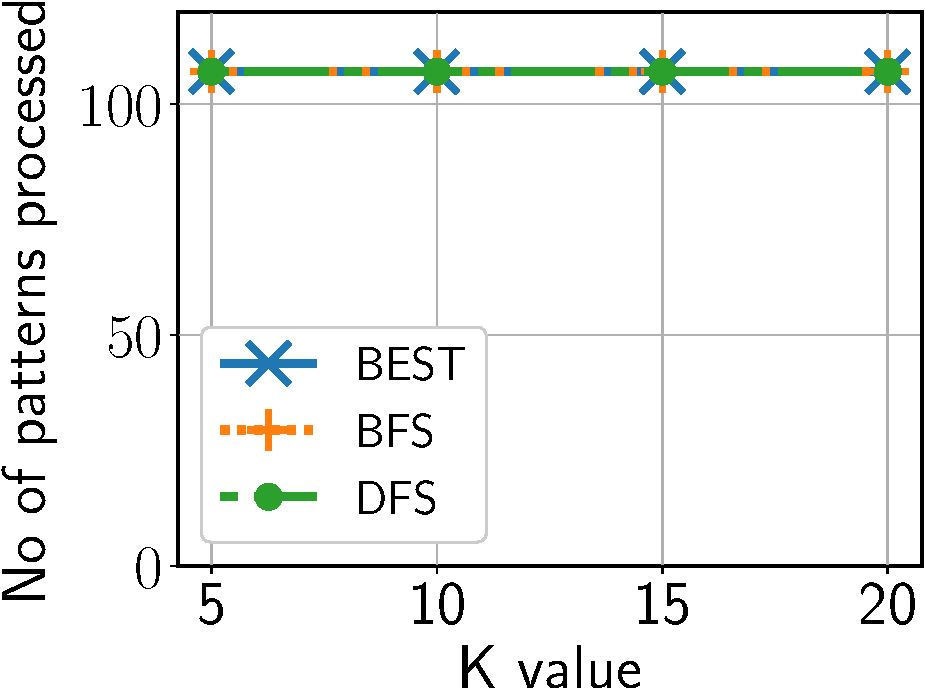
\includegraphics[keepaspectratio,scale=0.24, angle=0]{img2/citationdblp/citationdblp_bfsdfs_pop_k.pdf}}
\label{fig:chemical_bfsdfs_pop_k}
\vspace{-2mm}
\caption{\scriptsize Comparison with BFS and DFS.}
\label{fig:dbfs}
\vspace{-2mm}
\end{figure}




% \spara{$\bullet$ Index Analysis} We provide the result of efficiency increase of our global index. The index strategy is more powerful if there are fewer distinct edge labels or the data graph is more dense, like {\em Yeast} and {\em DBLP}.


% \begin{figure}[t!]
% \vspace{4mm}
% \centering
% \subfigure[{\scriptsize {\em Chemical} with {\sf Min-sup} = $10$, $k=50$}] {
% 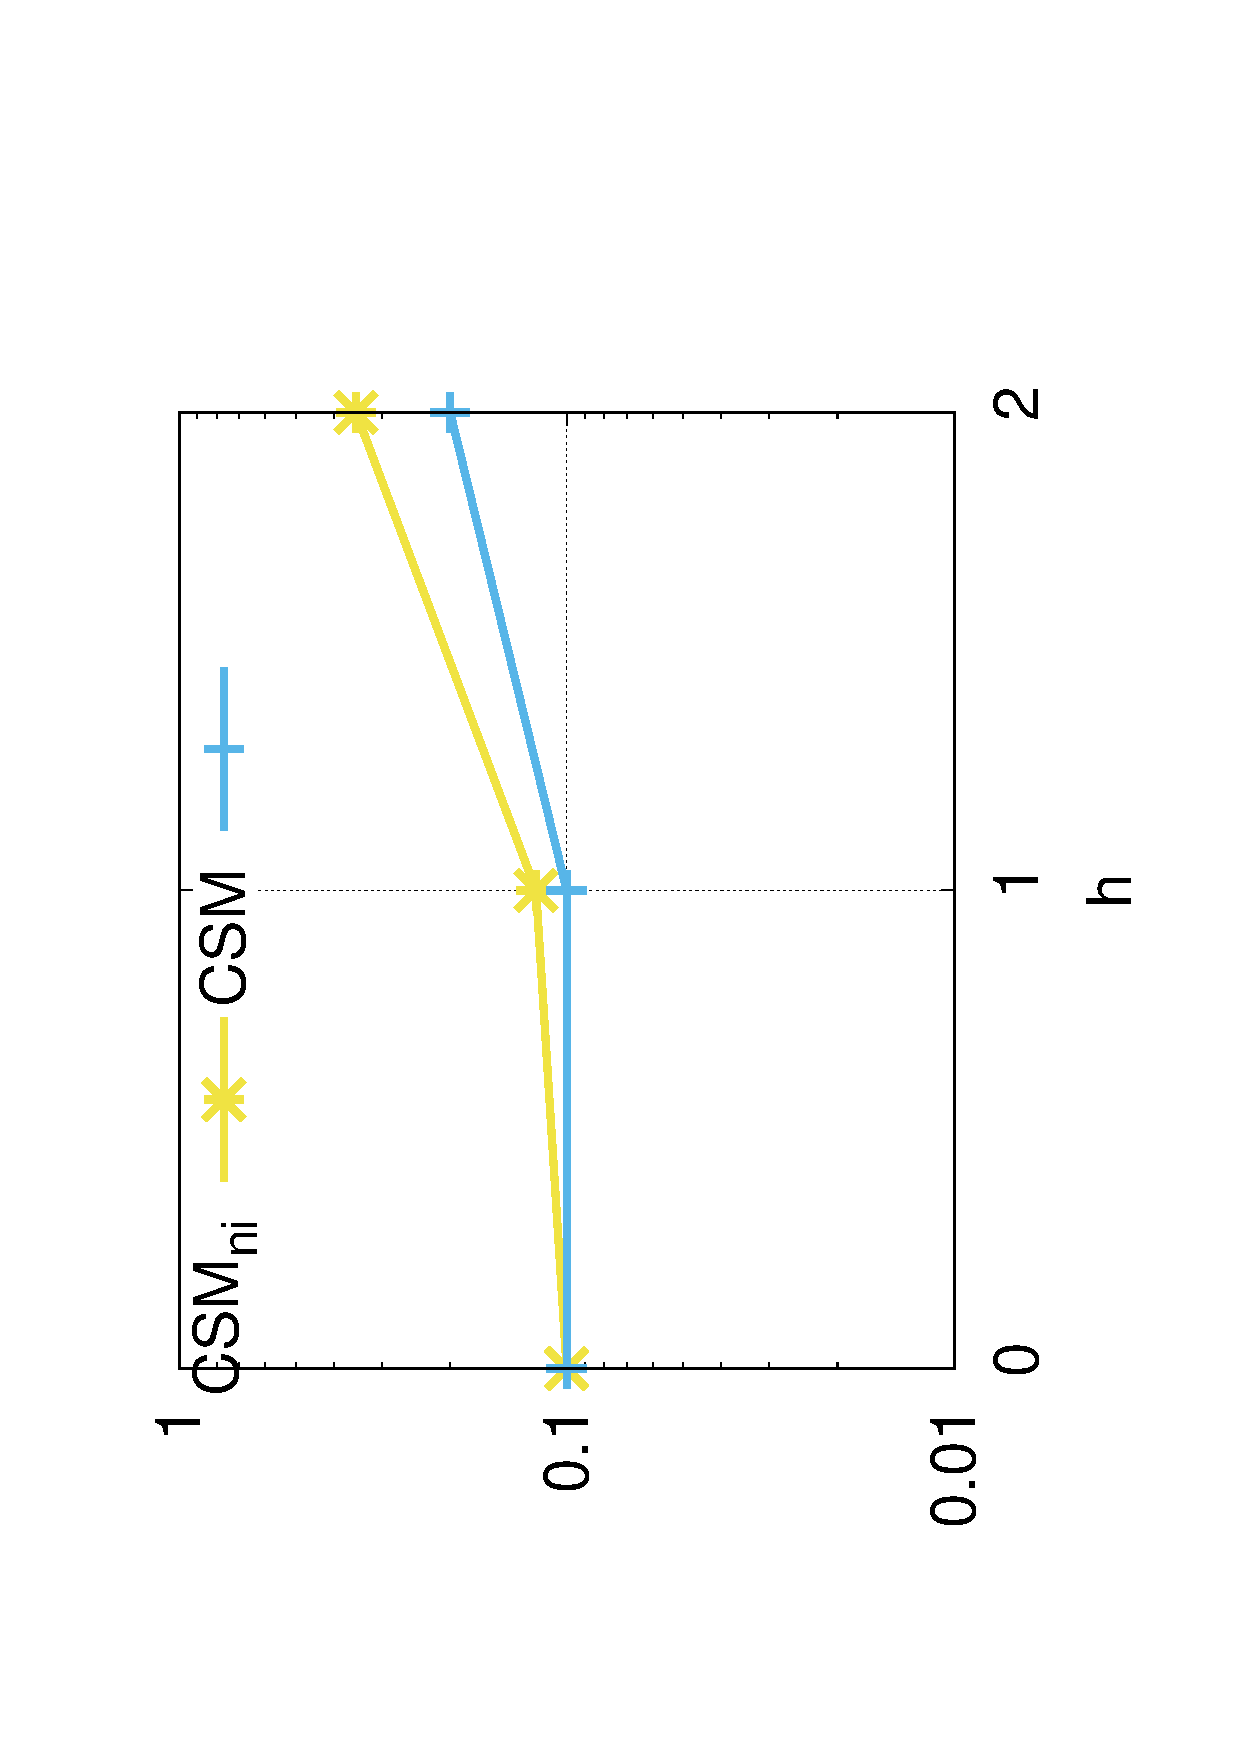
\includegraphics[scale=0.17, angle=270]{img2/ni_chemical}
% \label{fig:ni1}
% }
% \subfigure[{\scriptsize {\em Yeast} with {\sf Min-sup} = $200$, $k=50$}]  {
% \includegraphics[scale=0.17, angle=270]{img2/ni_yeast}
% \label{fig:ni2}
% }
% \subfigure[{\scriptsize {\em DBLP} with {\sf Min-sup} = $5000$, $k=50$}] {
% \includegraphics[scale=0.17, angle=270]{img2/ni_dblp}
% \label{fig:ni3}
% }
% \subfigure[{\scriptsize {\em LastFM} with {\sf Min-sup} = $200$, $k=50$}]  {
% \includegraphics[scale=0.17, angle=270]{img2/ni_lastfm}
% \label{fig:ni4}
% }
% \vspace{-2mm}
% \caption{\scriptsize Figure for index analysis.}
% \label{fig:ni}
% \vspace{-2mm}
% \end{figure}

\begin{figure}[t!]
\vspace{4mm}
\centering
\subfigure[{\scriptsize {\sf K}=$20$ in {\em LastFM}}] {
\includegraphics[keepaspectratio,scale=0.24, angle=0]{img2/lastfm/lastfm_kt.pdf}
\label{fig:lastfm_kt}
}
\subfigure[{\scriptsize {\sf K}=$20$ in {\em LastFM}}]  {
\includegraphics[keepaspectratio,scale=0.24, angle=0]{img2/lastfm/lastfm_spread.pdf}
\label{fig:lastfm_error}
}
\subfigure[{\scriptsize {\sf K}=$20$ in {\em Citeseer}}] {
\includegraphics[keepaspectratio,scale=0.24, angle=0]{img2/citeseer/citeseer_kt.pdf}
\label{fig:citeseer_kt}
}
\subfigure[{\scriptsize {\sf K}=$20$ in {\em Citeseer}}]  {
\includegraphics[keepaspectratio,scale=0.24, angle=0]{img2/citeseer/citeseer_spread.pdf}
\label{fig:citeseer_error}
}
\vspace{-2mm}
\caption{\scriptsize Qualitative Analysis.}
\label{fig:quality}
\vspace{-2mm}
\end{figure}


\subsection{Quality}
We show the quality of our approximation algorithm by comparing the results of top k of our approximate algorithm with the exact version, both run with a size bound of maximum 5 sized patterns. We take the output of the complete version as the ground truth for all the experiments. The following 3 experiments are done to show quality of our approximate version:
% \newline

\spara{Jaccard Coefficient.} We compare the patterns that we get in top-K in both the algorithms and report the fraction of pairs that we have in the approximate output which are there in the ground truth as well. The fraction comes out to be $1$ for all the datasets which means we get the exact same results as the exact version.

\spara{Kendall's Tau.} This is a measure of relationships between ranked data and focusses on the ordering of the results. It gives a value between 0-1 where 0 is no relationship and 1 is perfect relationship. It is calculated as \[KT = \dfrac{C-D}{C+D}, C = |concordant\ pairs|, D = |disconcordant\ pairs|\] Concordant pairs are how many larger ranks are below a certain rank and disconcordant pairs are how many smaller ranks are below a certain rank. We keep $K-20$ and show results of varied $hops$ at different supports for $LastFM$ in Figure \ref{fig:lastfm_kt}.\\ 

\spara{Percentage error in $\tau$ values.} This is a measure of the error in $\tau$ values introduced by the approximate version. We calculate the difference in the $\tau$ values for all the $top-K$ patterns common in the approximate and the exact set and report the mean error(in percentage). Figure \ref{fig:lastfm_error} shows this error at $K-20$ and varied $hops$ at different supports for $LastFM$.

\par We report quality metrics for the datasets at $K-20$, $Hop-1$ in Table \ref{tab:quality}. The support for every dataset is taken as the minimum support for the support ranges chosen for that dataset for the experiments. 

\begin{table}[tb!]
	\vspace{-2mm}
	\begin{center}
		\vspace{-1mm}
		\centering
		\caption{Quality metrics\label{tab:quality}}
		\vspace{-3mm}
		\begin{tabular} {cccc}
			\hline
			Datasets  & Jaccard Coeff & Kendall's Tau  & Percentage Error\\			 
			\hline 
			{\em Chemical}   &   1.0   &  1.0   & 0\\
			{\em Yeast}   &   1.0    &  0.75  & 0\\
			{\em MiCo}   &   1.0    &  1.0   & 0\\ 
			{\em LastFM}   &  1.0   &  1.0 & 0\\
			{\em DBLP Coauthor}   &   1.0  &  0.98  & 2.26\\ 
			{\em DBLP Citation}   &   1.0   &  1.0   & 0\\
			{\em Citeseer}   &   1.0   &  0.98 & 0\\
			
			\hline
		\end{tabular}
	\end{center}
	\vspace{-4mm}
\end{table}

\subsection{Interpretbility}

% \spara{$\bullet$ Further Analysis} We provide some further analysis. This part contains the result of the optimization of changing collection tree root in Section \ref{subsubsec:recursive}, and the time cost we spend to avoid the subgraph/supergraph correlations. According to the experimental result, the time we use to prune the not interesting correlations is about 10\% of the total time. Besides, the root changing optimization in Section \ref{subsubsec:recursive} increase the time efficiency by 10\%.


% \begin{figure}[t!]
% \vspace{4mm}
% \centering
% \subfigure[{\scriptsize {\em DBLP} with {\sf Min-sup} = $5000$, $h=2$}] {
% \includegraphics[scale=0.17, angle=270]{addimg/opt_dblp}
% \label{fig:opt1}
% }
% \subfigure[{\scriptsize {\em LastFM} with {\sf Min-sup} = $200$, $h=2$}]  {
% \includegraphics[scale=0.17, angle=270]{addimg/opt_lastfm}
% \label{fig:opt2}
% }
% \vspace{-2mm}
% \caption{\scriptsize Figure for further analysis.}
% \label{fig:opt}
% \vspace{-2mm}
% \end{figure}


% \spara{$\bullet$ Approximation Algorithm Analysis.} We provide the experimental result of our approximation mining algorithm.


% \begin{figure}[t!]
% \vspace{4mm}
% \centering
% \subfigure[{\scriptsize {\em DBLP} with {\sf Min-sup} = $5000$}] {
% \includegraphics[scale=0.17, angle=270]{addimg/a_dblp}
% \label{fig:ap1}
% }
% \subfigure[{\scriptsize {\em LastFM} with {\sf Min-sup} = $200$}]  {
% \includegraphics[scale=0.17, angle=270]{addimg/a_lastfm}
% \label{fig:ap2}
% }
% \vspace{-2mm}
% \caption{\scriptsize Figure for approximation algorithm analysis.}
% \label{fig:ap}
% \vspace{-2mm}
% \end{figure}



% \begin{figure}[t!]
% \vspace{-2mm}
% \centering
% \subfigure[{\scriptsize FSM on {\em Chemical}}] {
% \includegraphics[scale=0.17, angle=270]{img2/fsm_chemical}
% \label{fig:grami1}
% }
% \subfigure[{\scriptsize FSM on {\em Yeast}}]  {
% \includegraphics[scale=0.17, angle=270]{img2/fsm_yeast}
% \label{fig:grami2}
% }
% \subfigure[{\scriptsize FSM on {\em DBLP}}] {
% \includegraphics[scale=0.17, angle=270]{img2/fsm_dblp}
% \label{fig:grami3}
% }
% \subfigure[{\scriptsize FSM on {\em LastFM}}]  {
% \includegraphics[scale=0.17, angle=270]{img2/fsm_lastfm}
% \label{fig:grami4}
% }
% \subfigure[{\scriptsize a subgraph with 8 auto-morphisms}]  {
% \includegraphics[scale=0.3]{img2/grami5}
% \label{fig:grami5}
% }

% \vspace{-2mm}
% \caption{\scriptsize Comparison with {\sf GRAMI}.}
% \label{fig:grami}
% \vspace{-6mm}
% \end{figure}


% \spara{$\bullet$ Comparison with {\sf GRAMI}.} Additionally, we provide the efficiency analysis of the problem, frequent subgraph mining (FSM), of our approach {\sf CSM}, compared with the state-of-art approach of FSM in a single large graph, {\sf GRAMI}\cite{EASK14}. As the state-of-art FSM algorithm in a single large graph, {\sf GRAMI} transforms the subgraph isomorphism to a CSP (constraint satisfaction problem) and makes optimization based on it. Corresponding to our experiment result, in most of the conditions, {\sf GRAMI} has a higher efficiency due to that it does not need to find all the occurrances. However, {\sf GRAMI} could not a good performance dealing with some subgraphs since the most significant optimization, push-down prunning, could hardly contribute in this case (All the positions are valid domains of the subgraph pattern and there are totally $8$ isomorphisms using MNI metric in Figure \ref{fig:grami5}). 